\documentclass[a4paper,10pt]{article}
\usepackage[usenames,dvipsnames,svgnames,table]{xcolor}
\usepackage[includeheadfoot,pass,a4paper]{geometry}
\usepackage{datetime}
\usepackage{amssymb}
\usepackage{alphalph}
\usepackage{setspace}
\usepackage{graphicx}
\usepackage{tocstyle}
\usepackage{hyperref}
\usepackage{multicol}
\usepackage{import}
\usepackage{wallpaper}
\usepackage{tikz}
\usepackage{parcolumns}
\usepackage{multirow}
\usepackage{changepage}
\usepackage{titlesec}
\usepackage{tocvsec2}
\usepackage{enumitem}
\usepackage{paralist}
\usepackage{pdftexcmds}
\usepackage{wrapfig}
\usepackage{subcaption}
\usepackage{booktabs}
\usepackage{fancyhdr}
\usepackage{lastpage}
\usepackage{xstring}
\usepackage{minitoc}
\usepackage{pagecolor}
\usepackage{pdfpages}
\usepackage[toc,nopostdot,nonumberlist,style=altlistgroup]{glossaries}
\usepackage{hyphenat}
\usepackage[space]{grffile}
\usepackage{rotating}
\usepackage{pdflscape}
\usetikzlibrary{calc}

%----------------------------------------------------------------------------------------
%   VARIABLES
%----------------------------------------------------------------------------------------
\newdateformat{mydate}{\monthname[\THEMONTH] \ordinaldate{\THEDAY}, \THEYEAR{ }}

\newcommand{\documentVersion}{v1.0.0-08.31.2018}
\newcommand{\documentSubTitle}{System and Software Life Cycle Processes}
\newcommand{\documentTitle}{Common Framework for Life Cycles and their Processes}
\newcommand{\documentBackground}{../Boilerplate/Background/document-background-print.png}
\newcommand{\copyrightClause}{\copyright{} Remix $|$ A3RK $|$ Vox Populi, Vox Monetae}


%----------------------------------------------------------------------------------------
%   MARGINS, TEXT, TITLES
%----------------------------------------------------------------------------------------

\topmargin -1.25cm        
\oddsidemargin -0.65cm   
\evensidemargin 0cm  
\textwidth 17.2cm
\textheight 23.75cm 
\parskip 5pt          
\parindent 0pt 

\titleformat{\section}[block]{\bfseries}{\thesection.}{1em}{}
\titleformat{\subsection}[block]{\bfseries}{\thesubsection}{1em}{}
\titleformat{\subsubsection}[block]{\bfseries}{\thesubsubsection}{1em}{}
\titlespacing*{\subsection} {0.5em}{1.25ex plus 1ex minus .2ex}{1.5ex plus .2ex}
\titlespacing*{\subsubsection} {1em}{1.25ex plus 1ex minus .2ex}{1.5ex plus .2ex}

%----------------------------------------------------------------------------------------
%   TEXT COLOR
%----------------------------------------------------------------------------------------

\definecolor{articleColor}{cmyk}{0 , 0  , 0   , 0.85}
\color{articleColor}

%----------------------------------------------------------------------------------------
%   SPACING
%----------------------------------------------------------------------------------------

\onehalfspacing

%----------------------------------------------------------------------------------------
%   EXTENDED LISTS
%----------------------------------------------------------------------------------------

\renewcommand{\labelenumi}{\arabic{enumi}. }
\renewcommand{\labelenumii}{\arabic{enumii}. }
\renewcommand{\labelenumiii}{\arabic{enumiii}. }


%----------------------------------------------------------------------------------------
%   HEADER AND FOOTER
%----------------------------------------------------------------------------------------

\pagestyle{fancy} 
\fancyhf{}
\renewcommand{\headrulewidth}{0pt}
\renewcommand{\footrulewidth}{0.25pt}

\fancyfoot[CE,LO]{
		{\scriptsize 
				\documentSubTitle \\[0.35ex]  
				\textbf{\documentTitle{}} \\[0.35ex] 
				\copyrightClause{} \\[0.35ex] 
		}
}

\fancyfoot[LE,RO]{
		{\scriptsize 
				\hfill Page \thepage{} of \pageref{LastPage} \\[0.35ex] 
				\textbf{ } \\[0.35ex]
				\hyperref[sec:changelog]{\documentVersion{}}\\[0.35ex]
		}
}
%----------------------------------------------------------------------------------------
%   TITLE PAGE
%----------------------------------------------------------------------------------------

\newcommand*{\titleGM}{\begingroup 
\hbox{ 
\parbox[b]{1\textwidth}{
\vspace{0.03\textheight} 
{\noindent\Large\bfseries \documentTitle}\\[1\baselineskip]
{\large \textit{\documentSubTitle}}\\[4\baselineskip]

}}
\endgroup}

%----------------------------------------------------------------------------------------
%   BACKGROUND
%----------------------------------------------------------------------------------------

\CenterWallPaper{1}{\documentBackground}

%----------------------------------------------------------------------------------------
%   SUBSUBSUBSECTIONS
%----------------------------------------------------------------------------------------

\titleclass{\subsubsubsection}{straight}[\subsection]

\newcounter{subsubsubsection}[subsubsection]
\renewcommand\thesubsubsubsection{\thesubsubsection.\arabic{subsubsubsection}}
\renewcommand\theparagraph{\thesubsubsubsection.\arabic{paragraph}} % optional; useful if paragraphs are to be numbered

\titleformat{\subsubsubsection}[block]{\normalfont\normalsize\bfseries}{\thesubsubsubsection}{1em}{}
\titlespacing*{\subsubsubsection} {1.5em}{3.25ex plus 1ex minus .2ex}{1.5ex plus .2ex}

\makeatletter
\renewcommand\paragraph{\@startsection{paragraph}{6}{\z@}%
	{1.25ex \@plus1ex \@minus.2ex}%
	{-1em}%
	{\normalfont\normalsize\bfseries}}
\renewcommand\subparagraph{\@startsection{subparagraph}{7}{\parindent}%
	{1.25ex \@plus1ex \@minus .2ex}%
	{-1em}%
	{\normalfont\normalsize\bfseries}}
\def\toclevel@subsubsubsection{4}
\def\toclevel@paragraph{5}
\def\toclevel@paragraph{6}
\def\l@subsubsubsection{\@dottedtocline{4}{7em}{4em}}
\def\l@paragraph{\@dottedtocline{5}{10em}{5em}}
\def\l@subparagraph{\@dottedtocline{6}{14em}{6em}}
\makeatother

%----------------------------------------------------------------------------------------
%   SUBSUBSUBSECTIONS
%----------------------------------------------------------------------------------------

\titleclass{\subsubsubsubsection}{straight}[\subsection]

\newcounter{subsubsubsubsection}[subsubsubsection]
\renewcommand\thesubsubsubsubsection{\thesubsubsubsection.\arabic{subsubsubsubsection}}
\renewcommand\theparagraph{\thesubsubsubsubsection.\arabic{paragraph}} % optional; useful if paragraphs are to be numbered

\titleformat{\subsubsubsubsection}[block]{\normalfont\normalsize\bfseries}{\thesubsubsubsubsection}{1em}{}
\titlespacing*{\subsubsubsubsection} {3em}{3.25ex plus 1ex minus .2ex}{1.5ex plus .2ex}

\makeatletter
\renewcommand\paragraph{\@startsection{paragraph}{6}{\z@}%
	{1.25ex \@plus1ex \@minus.2ex}%
	{-1em}%
	{\normalfont\normalsize\bfseries}}
\renewcommand\subparagraph{\@startsection{subparagraph}{7}{\parindent}%
	{1.25ex \@plus1ex \@minus .2ex}%
	{-1em}%
	{\normalfont\normalsize\bfseries}}
\def\toclevel@subsubsubsubsection{5}
\def\toclevel@paragraph{6}
\def\toclevel@paragraph{7}
\def\l@subsubsubsubsection{\@dottedtocline{5}{8em}{4em}}
\def\l@paragraph{\@dottedtocline{6}{12em}{5em}}
\def\l@subparagraph{\@dottedtocline{7}{16em}{6em}}
\makeatother

\setcounter{secnumdepth}{8}
\setcounter{tocdepth}{60}

\newcommand{\itab}[1]{\hspace{0em}\rlap{#1}}
\newcommand{\tab}[1]{\hspace{.2\textwidth}\rlap{#1}}


%----------------------------------------------------------------------------------------
%   DOCUMENT
%----------------------------------------------------------------------------------------
\begin{document}

	\titleGM
	\newpage

	\tableofcontents
	\newpage

	\section{CHANGELOG\label{sec:changelog}}
\begin{adjustwidth}{0em}{0pt}

	This document, in being heavily cited and used as a handbook and guiding force for entire organizations and the vast majority of currently active initiatives, will be updated regularly based on its usage and the need for it to be further extended, modified, refined, and so on. 

	The versioning of the document shall adhere to the most common form of software versioning, where the major version is followed by a decimal point and a minor version and the minor version is followed by a decimal point and a release or build version (major.minor.build). In this context, major versions shall be released when document-wide reorganization or deprecation is required, minor versions shall be released when sections or appendices are added, removed, or modified in ways that require they be merged, broken apart, or renamed, and builds shall be released when any change is made to the document itself. 

	Furthermore, the date of the release shall be appended to the major.minor.build form, separated by a dash. e.g. 1.0.0-08.31.2018 is the first version, first release, that occurred on August 31st, 2018. Note that this information may always be found in the bottom right-hand corner of every page of this document.

	The source code for the document is written in LaTeX, and the author of the document would request it remain in that format so as to facilitate quick revision and release. 

	\begin{compactitem}

		\item {\bf v1.0.0-08.31.2018}: initial release of document and exposure of proposed framework for process definition and reference modeling. 

	\end{compactitem}

\end{adjustwidth}

	\newpage
	\section{INTRODUCTION}
\begin{adjustwidth}{0em}{0pt}

	This standard establishes a common framework for life cycle processes, with well-defined terminology, that can be referenced by businesses, organizations, and entities that create, manage, and provide software directly or indirectly, as a part of, or wholly comprising, their purchasable products and services, regardless of the industry in which the business itself is classified or categorized. 

	This standard applies to the acquisition of systems and software products and services, to the supply, development, operation, maintenance, and disposal of software products and the software portion of a system, whether performed internally or externally to an organization. Those aspects of system definition needed to provide the context for software products and services, and a process that can be employed for defining, controlling, and improving software life cycle processes, are provided herein. The processes may also be applied during the acquisition of a system that contains software.

	This standard can be used in one or more of the following modes:\\

		\begin{compactitem}

			\item {\bf By an organization} - to help establish an environment of desired processes. These processes can be supported by an infrastructure of methods, procedures, techniques, tools, and trained personnel. The organization may then employ this environment to perform and manage its projects and progress systems through their life cycle stages. In this more, this book is used to assess conformance of a declared, established set of life cycle processes to its provisions. \\

			\item {\bf By a project} - to help select, structure, and employ the elements of an established set of life cycle processes to provide products and services. In this more, this book is used in the assessment of conformance of the project to the declared and established environment. \\

			\item {\bf By an acquirer and a supplier} - to help develop an agreement concerning processes and activities. Via the agreement, the processes and activities in this book are selected, negotiated, agreed to, and performed. In this mode, this book is used for guidance in developing the agreement. \\

			\item {\bf By organizations and assessors} - to perform assessments that may be used to support organizational process improvement.

		\end{compactitem}

\end{adjustwidth} 

	\newpage
	\section{UNDERSTANDING AND APPLYING THIS STANDARD}

	\subsection{RELATIONSHIP BETWEEN SYSTEMS AND SOFTWARE}
	\begin{adjustwidth}{0.5em}{0pt}

		This standard establishes a strong link between a system and its software. It is based upon the general principles of systems engineering. Software is treated as an integral part of the total system and performs certain functions in that system. This is implemented by extracting the software requirements from the system requirements and design, producing the software, and integrating it into the system. 

		It is a fundamental premise that software always exists in the context of a system, even if the system consists of only the processor upon which the software is executed. Therefore, a software product or service is always treated as one item in a system. 

		For example, this standard makes a distinction between system requirements analysis and software requirements analysis, because, in the general case, system architectural design will allocate the system requirements to various items of the system and software requirements analysis will derive software requirements from the system requirements allocated to each software item. 

		Note that in some cases, the non-software items of a system may be so minimal that it may not be necessary to perform distinct system and software analyses.

	\end{adjustwidth}

	\subsection{ORGANIZATION-LEVEL AND PROJECT-LEVEL ADOPTION}
	\begin{adjustwidth}{0.5em}{0pt}

		Modern software businesses strive to develop an exhaustive set of software life cycle processes that are applied repeatedly to the software projects of the business. Therefore, this standard is intended to be useful for adoption at either the organization level or at the project level. 

		An organization would adopt this standard and supplement it with appropriate procedures, practices, tools and policies. 

		A software project of the organization would conform to the organization's processes rather than conform directly to this standard. 

		In some cases, projects may be executed by an organization that does not have an appropriate set of processes adopted at the organizational level. Such a project may apply the provisions of this standard directly to the project itself.

	\end{adjustwidth}

	\subsection{TEMPORAL RELATIONSHIPS AMONG PROCESSES}
	\begin{adjustwidth}{0.5em}{0pt}

		Within this standard, the processes and their activities and tasks are arranged in a sequence suitable for exposition. This positional sequence does not prescribe or dictate any time-dependent sequence. 

		For lack of consensus on or use of a universal time-dependent sequence, the reader may select and order the processes, activities, and tasks as appropriate and effective. 

		This standard encourages iteration among the activities and recursion within an activity to offset the effects of any implied sequence of activities and tasks. 

		The organization is ultimately responsible for selecting a life cycle model for the project and mapping the processes, activities, and tasks onto that model, as well as for selecting life cycle models and processes for its own internal management and governance belonging to, or wholly separate from, those used for software projects. 

	\end{adjustwidth}


	\subsection{EVALUATION VS VERIFICATION AND VALIDATION}
	\begin{adjustwidth}{0.5em}{0pt}

		Organizations that are involved in any process of a life cycle conduct evaluations of the products of that task. The Software Verification and Software Validation processes provide the opportunity for additional evaluations. These processes are conducted by the acquirer, the supplier, or an independent party to verify and validate the products in varying depth depending on the project. 

		These evaluations do not duplicate or replace other evaluations, but supplement them. Additional opportunities for evaluation are provided by the Software Review, Software Audit, Software Quality Assurance and the Life Cycle Model Management Processes.

	\end{adjustwidth}


	\subsection{CRITERIA FOR PROCESSES}
	\begin{adjustwidth}{0.5em}{0pt}

		This standard establishes a framework for the life cycle of software. The life cycle begins with an idea or a need that can be satisfied wholly or partly by software and ends with the retirement of the software. The architecture is built with a set of processes and interrelationships among these processes. The determination of the life cycle processes is based upon two basic principles: cohesion and responsibility.\\

		\begin{compactitem}

			\item {\bf Cohesion}: The life cycle processes are cohesive and coupled to the optimum extent deemed practical and feasible \\

			\item {\bf Responsibility}: A process is placed under the responsibility of an organization or role in the software life cycle\\

		\end{compactitem}

	\end{adjustwidth}


	\subsection{DESCRIPTION AND GENERAL CHARACTERISTICS OF PROCESSES}
	\begin{adjustwidth}{0.5em}{0pt}

		The processes within this standard are described in a manner that is meant to facilitate the use of this standard for either, or both, organization-level and project-level adoption. Each process is described in terms of the following attributes:\\

		\begin{compactitem}

			\item {\bf Title}: The title conveys the scope of the process as a whole\\

			\item {\bf Purpose}: The purpose describes the goals of performing the process\\

			\item {\bf Outcomes}: The outcomes express the observable results expected from the successful performance of the process\\

			\item {\bf Activities}: The activities are a list of actions that are used to achieve the outcomes\\

			\item {\bf Tasks}: The tasks are requirements, recommendations, or permissible actions intended to support the achievement of the outcomes\\

		\end{compactitem}

	\end{adjustwidth}


	\subsection{DECOMPOSITION OF PROCESSES}
	\begin{adjustwidth}{0.5em}{0pt}

		Each process within this standard satisfies the criteria described above. For the purpose of clear description,processes are sometimes decomposed into smaller pieces. Some processes are decomposed into activities and/or lower-level processes. A lower-level process is described when the decomposed portion of the process itself satisfies the criteria to be a process. An activity is used when the decomposed unit does not qualify as a process. An activity can be considered as simply a collection of tasks.

		A task is expressed in the form of a requirement, recommendation, or permissible action, intended to support the achievement of the outcomes of a process. For this purpose, this standard carefully employs certain auxiliary verbs (shall, should, and may) to differentiate between the distinct forms of a task. ``Shall'' is used to express a provision required for conformance, ``should'' to express a recommendation among other possibilities, and ``may'' to indicate a course of action permissible within the limits of this standard and common framework.

	\end{adjustwidth}


	\subsection{LIFE CYCLE MODELS AND STAGES}
	\begin{adjustwidth}{0.5em}{0pt}

		The life of a system or a software product can be modeled by a life cycle model consisting of stages. Models may be used to represent the entire life from concept to disposal or to represent the portion of the life corresponding to the current project. The life cycle model is comprised of a sequence of stages that may overlap and/or iterate, as per the project's scope, magnitude, complexity, changing needs and opportunities. 

		Each stage is described with a statement of purpose and outcomes. The life cycle processes and activities are selected and employed in a stage to fulfill the purpose and outcomes of that stage. 

		Different organizations may undertake different stages in the life cycle. However, each stage is conducted by the organization responsible for that stage with due consideration of the available information on life cycle plans and decisions made in preceding stages. Similarly, the organization responsible for that stage records the decisions made and records the assumptions regarding subsequent stages in the life cycle.

		Finally, this standard does not dictate the use of any specific combination or permutation of stages to explicitly and always define any given life cycle. It is left to the organization to determine, by using this standard and its examples and exhaustive breakdown and definition of life cycle processes, those life cycles beneath their own business operations and processes, their own tactical initiatives, activities, and tasks. 

	\end{adjustwidth}

	\newpage
	\section{STRUCTURE, ORGANIZATION, AND IMPLEMENTATION}

	\subsection{CATEGORIES OF LIFE CYCLE PROCESSES}

	\begin{figure}[h]
		\centering
		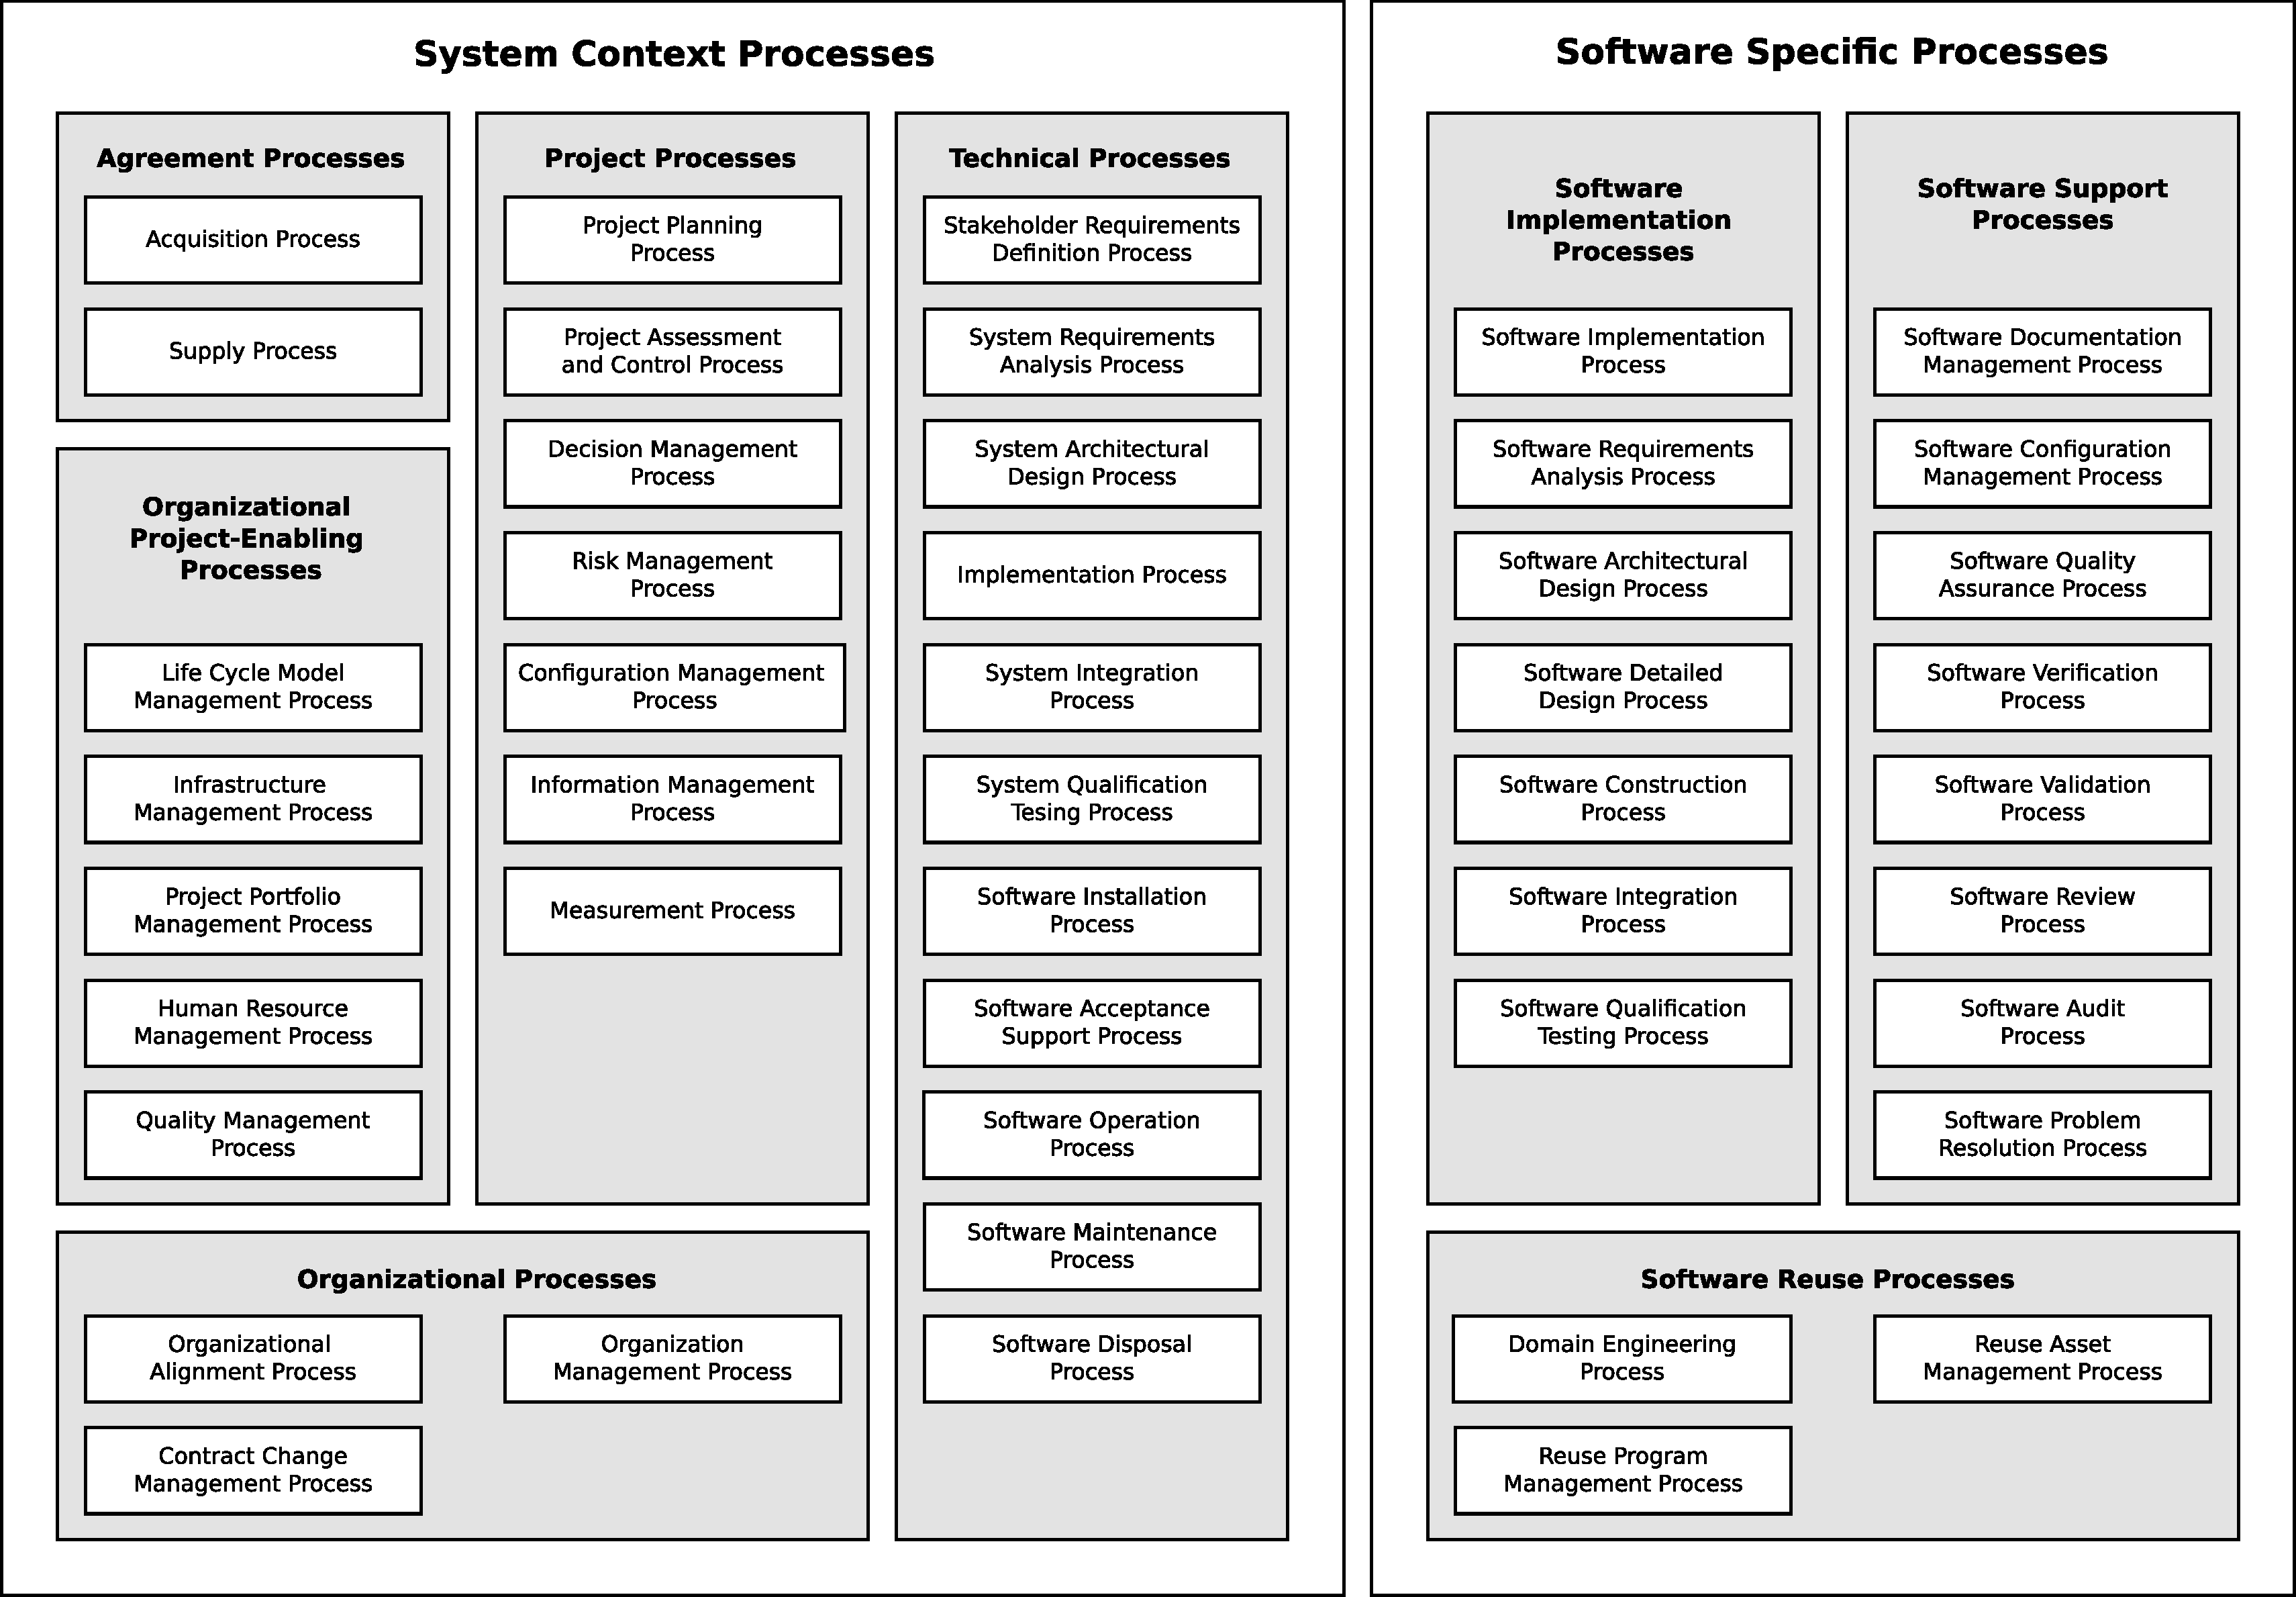
\includegraphics[width=17cm,keepaspectratio]{figures/life-cycle-process-groups.pdf}
		\caption{Process Reference Model (PRM)}
		\label{fig:life_cycle_process_groups}
	\end{figure}

	\begin{adjustwidth}{0.5em}{0pt}

		To facilitate practical understanding and application of this standard, we have grouped the activities that may be performed during the life cycle of a software system into seven process groups. Each of the life cycle processes within those groups is described in terms of its purpose and desired outcomes, and lists activities and tasks which need to be performed to achieve those outcomes.

		The purpose and outcomes of the life cycle processes constitute a Process Reference Model (PRM), where each process group is contained within its own distinct section, the process groups and their processes are sub-sections within those sections, and each sub-section / process contains sub-sub-sections for their purpose, outcome, activities, and tasks. 

	\end{adjustwidth}

	\subsection{SUMMARY OF LIFE CYCLE PROCESSES}
	\begin{adjustwidth}{0.5em}{0pt}

		There are two major sub-divisions of process within this standard, where Section \nameref{sec:system_context_processes} provides a system context for dealing with a standalone software product or service of a software system, and Section \nameref{sec:software_specific_processes} contains the software-specific processes for use in implementing a software product or service that is an element of a larger system. Brief summarization of these divisions' process groups may be found below.

	\end{adjustwidth}

		\subsubsection{AGREEMENT PROCESSES}
		\begin{adjustwidth}{1em}{0pt}

			\nameref{subsec:agreement_processes} define the activities necessary to establish an agreement between two organizations. 

		\end{adjustwidth}

		\subsubsection{ORGANIZATIONAL PROJECT-ENABLING PROCESSES}
		\begin{adjustwidth}{1em}{0pt}

			The \nameref{subsec:organizational_project_enabling_processes} manage the organization's capability to acquire and supply products or services through the initiation, support and control of projects. They provide resources and infrastructure necessary to support projects and ensure the satisfaction of organizational objectives and established agreements.

		\end{adjustwidth}

		\subsubsection{PROJECT PROCESSES}
		\begin{adjustwidth}{1em}{0pt}

			There are two categories of \nameref{subsec:project_processes}. The Project Management Processes are used to plan, execute, assess and control the progress of a project. The Project Support Processes support specialized management objectives.

		\end{adjustwidth}

		\subsubsection{ORGANIZATIONAL PROCESSES}
		\begin{adjustwidth}{1em}{0pt}

			The \nameref{subsec:organizational_processes} are highly useful, in that they help organizations ensure their processes are aligned and consistent with its business goals.

		\end{adjustwidth}

		\subsubsection{TECHNICAL PROCESSES}
		\begin{adjustwidth}{1em}{0pt}

			The \nameref{subsec:technical_processes} are used to define the requirements for a system, to transform the requirements into an effective product, to permit consistent reproduction of the product where necessary, to use the product, to provide the required services, to sustain the provision of those services and to dispose of the product when it is retired from service.

		\end{adjustwidth}

		\subsubsection{SOFTWARE IMPLEMENTATION PROCESSES}
		\begin{adjustwidth}{1em}{0pt}

			The \nameref{subsec:software_implementation_processes} are used to produce a specified system element (software item) implemented in software. 

			Those processes transform specified behavior, interfaces and implementation constraints into implementation actions resulting in a system element that satisfies the requirements derived from the system requirements.

		\end{adjustwidth}

		\subsubsection{SOFTWARE SUPPORT PROCESSES}
		\begin{adjustwidth}{1em}{0pt}

			The \nameref{subsec:software_support_processes} provide a specific focused set of activities for performing a specialized software process. A supporting process assists the Software Implementation Process as an integral part with a distinct purpose, contributing to the success and quality of the software project.

		\end{adjustwidth}

		\subsubsection{SOFTWARE REUSE PROCESSES}
		\begin{adjustwidth}{1em}{0pt}

			The \nameref{subsec:software_reuse_processes} consists of three processes that support an organization's ability to reuse software items across project boundaries. These processes are unique because, by their nature, they operate outside the bounds of any particular project.

		\end{adjustwidth}


	\subsection{STANDARD AS PROCESS REFERENCE MODEL (PRM)}
	\begin{adjustwidth}{0.5em}{0pt}

		A Process Reference Model (PRM) provides a level of abstraction higher than that of the detailed required contained with any given standard or specification, and is applicable to an organization that is assessing its processes in order to determine their own capabilities and limitations. 
		
		A Process Reference Model, by definition, must contain the following:

		\begin{compactenum}

			\item A declaration of the target domain

			\item A description of the processes within its scope

			\item A description of the relationship between itself and its intended context of use

			\item A description of the relationship between the processes defined within itself

		\end{compactenum}


		A Process Reference Model does not necessarily represent a particular process implementation approach, nor does it prescribe a system/software life cycle model, methodology, or technique. Instead, the reference model is intended to be adopted by an organization based on its business needs and application domain. 

		Furthermore, the organization's defined process is adopted by the organization's projects in the context of the projects' requirements. 

		In order to ensure this standard serves as a legitimate Process Reference Model, it has been written and structured in a manner and method that satisfies international standards and guidelines while also, hopefully, being informative, educational, and useful to its readers. 

	\end{adjustwidth}

	\newpage
	\section{SYSTEM CONTEXT PROCESSES \label{sec:system_context_processes}}

	\subsection{AGREEMENT PROCESSES\label{subsec:agreement_processes}}

	\begin{figure}[h]
		\centering
		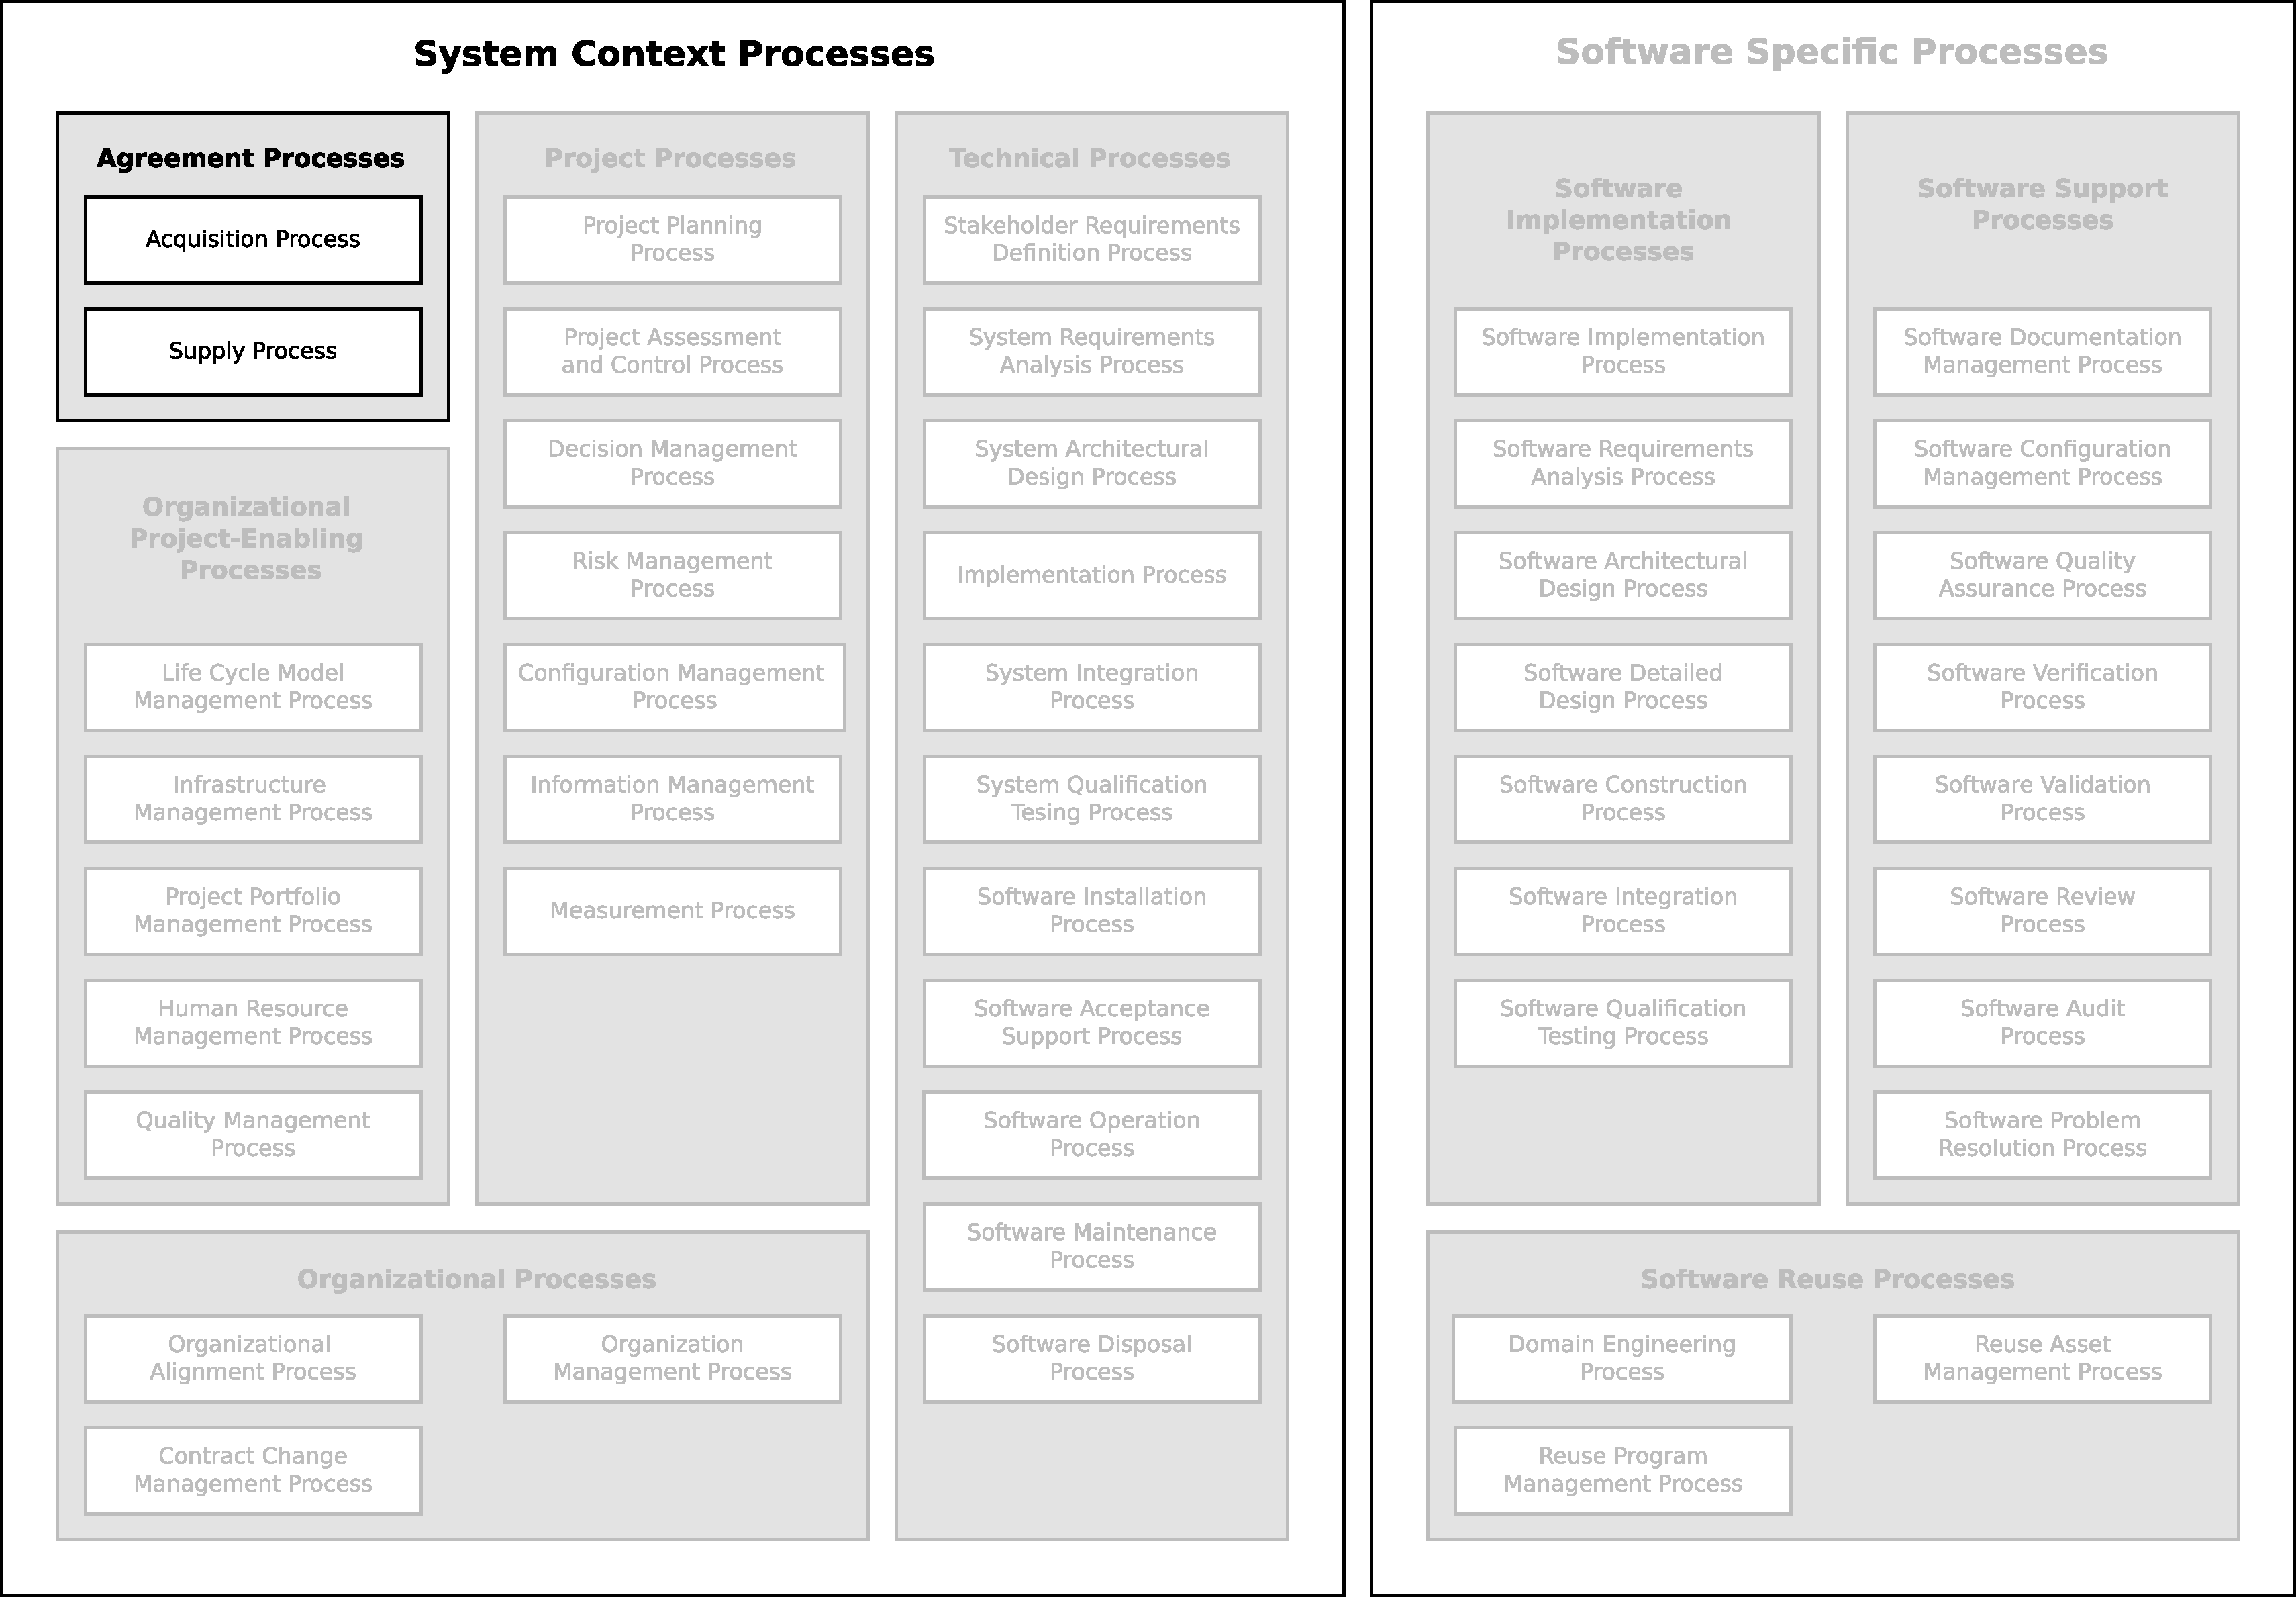
\includegraphics[width=15cm,keepaspectratio]{figures/life-cycle-process-groups-agreement-processes.pdf}
		\caption{Agreement Processes}
		\label{fig:agreement_processes}
	\end{figure}

	\begin{adjustwidth}{1em}{0pt}

		If the \nameref{proc:acquisition_process} is invoked, it provides the means for conducting business with a supplier of products that are supplied for use as an operational system, of services in support of an operational system, or of elements of a system being developed by a project. 

		If the \nameref{proc:supply_process} is invoked, it provides the means for conducting a project in which the result is a product or service that is delivered to the acquirer.

		In this Section:

		\begin{compactitem}
			\item \ref{proc:acquisition_process} - \nameref{proc:acquisition_process}
			\item \ref{proc:supply_process} - \nameref{proc:supply_process}
		\end{compactitem}

	\end{adjustwidth}

		\newpage
		\subsubsection{ACQUISITION PROCESS\label{proc:acquisition_process}}

			\subsubsubsection{PURPOSE}
			\begin{adjustwidth}{2em}{0pt}

				The purpose of the Acquisition Process is to obtain the product and/or service that satisfies the need expressed by the acquirer. The process begins with the identification of customer needs and ends with the acceptance of the product and/or service needed by the acquirer. 

			\end{adjustwidth}

			\subsubsubsection{OUTCOMES}
			\begin{adjustwidth}{2em}{0pt}

				\begin{compactitem}
					\item acquisition needs, goals, product and/or service acceptance criteria and acquisition strategies are defined;

					\item an agreement is developed that clearly expresses the expectation, responsibilities and liabilities of both the acquirer and the supplier;

					\item one or more suppliers is selected;

					\item a product and/or service is acquired that satisfies the acquirer's stated need
					
					\item the acquisition is monitored so that specified constraints such as cost, schedule and quality are met;
					
					\item supplier deliverables are accepted; and
					
					\item any identified open items have a satisfactory conclusion as agreed to by the acquirer and the supplier. 
				\end{compactitem}

			\end{adjustwidth}

			\subsubsubsection{ACTIVITIES AND TASKS}
			\begin{adjustwidth}{2em}{0pt}

				\begin{compactenum}

					\item {\bf Acquisition Preparation}

					\begin{compactenum}
						\item The acquirer begins the acquisition process by describing a concept or a need to acquire, develop, or enhance a system, software product or software service.

						\item The acquirer shall define and analyze the system requirements. The system requirements should include business, organizational and user as well as safety, security, and other criticality requirements along with related design, testing, and compliance standards and procedures.

						\item The acquirer may perform the definition and analysis of software requirements by itself or may retain a supplier to perform this task.

						\item If the acquirer retains a supplier to perform system or software requirements analysis, the acquirer shall retain approval authority for the analyzed requirements.

						\item The Technical Processes should be used to perform the tasks above. The acquirer may use the Stakeholder Requirements Definition Process to establish the customer requirements.

						\item The acquirer shall consider options for acquisition against analysis of appropriate criteria to include risk, cost and benefits for each option. Options include:

						\begin{compactitem}
							\item Purchase an off-the-shelf software product that satisfies the requirements.
							\item Develop the software product or obtain the software service internally.
							\item Develop the software product or obtain the software service through contract.
							\item A combination of the three items above.
							\item Enhance an existing software product or service.
						\end{compactitem}

						\item When an off-the-shelf software product is to be acquired, the acquirer shall ensure the following conditions are satisfied:

						\begin{compactitem}
							\item The requirements for the software product are satisfied.
							\item The required documentation is available.
							\item Proprietary, usage, ownership, warranty and licensing rights are satisfied.
							\item Future support for the software product is planned.
						\end{compactitem}

						\item The acquirer should prepare, document and execute an acquisition plan. The plan should contain the following:

						\begin{compactitem}
							\item Requirements for the system.
							\item Planned employment of the system.
							\item Type of contract to be employed.
							\item Responsibilities of the organizations involved.
							\item Support concept to be used.
							\item Risks considered as well as methods to manage the risks.
						\end{compactitem}

						\item The acquirer shall define and document the acceptance strategy and conditions (criteria).

						\item The acquirer should document the acquisition requirements (e.g., request for proposal), the content of which depends upon the acquisition option selected in previously defined task. The acquisition documentation should include, as appropriate:

						\begin{compactitem}
							\item System requirements.
							\item Scope statement.
							\item Instructions for bidders.
							\item List of software products.
							\item Terms and conditions.
							\item Control of subcontracts.
							\item Technical constraints (e.g. target environment).
						\end{compactitem}

						\item The acquirer should determine which processes of this standard are appropriate for the acquisition and specify any acquirer requirements for tailoring those processes. The acquirer should specify if any of the processes are to be performed by parties other than the supplier, so that suppliers may, in their proposals, define their approach to supporting the work of other parties. The acquirer shall define the scope of those tasks that reference the contract.

						\item The acquisition documentation shall also define the contract milestones at which the supplier's progress shall be reviewed and audited as part of monitoring the acquisition.

						\item The acquisition requirements should be given to the organization selected for performing the acquisition activities.
					\end{compactenum}

					\item {\bf Acquisition Advertisement}
					\begin{compactenum}
						\item The acquirer shall communicate the request for the supply of a product or service to identified suppliers. 
					\end{compactenum}

					\item {\bf Supplier Selection}
					\begin{compactenum}
						\item The acquirer should establish a procedure for supplier selection including proposal evaluation criteria and requirements compliance weighting.

						\item The acquirer should select a supplier based upon the evaluation of the suppliers' proposals, capabilities, and in accordance with the acquirer's acceptance strategy and conditions.
					\end{compactenum}

					\item {\bf Contract Agreement}
					\begin{compactenum}
						\item The acquirer may involve other parties, including potential suppliers or any necessary third parties (such as regulators), before contract award, in determining the acquirer's requirements for tailoring of this standard for the project. In making this determination, the acquirer shall consider the effect of the tailoring requirements upon the supplier's organizationally-adopted processes. The acquirer shall include or reference the tailoring requirements in the contract.

						\item The acquirer shall then prepare and negotiate a contract with the supplier that addresses the acquisition requirements, including the cost and schedule, of the software product or service to be delivered. The contract shall address proprietary, usage, ownership, warranty and licensing rights associated with the reusable off-the-shelf software products.

						\item Once the contract is underway, the acquirer shall control changes to the contract through negotiation with the supplier as part of a change control mechanism. Changes to the contract shall be investigated for impact on project plans, costs, benefits, quality, and schedule.
					\end{compactenum}

					\item {\bf Agreement Monitoring}
					\begin{compactenum}
						\item The acquirer shall monitor the supplier's activities in accordance with the Software Review Process and the Software Audit Process. The acquirer should supplement the monitoring with the Software Verification Process and the Software Validation Process as needed. 

						\item The acquirer shall cooperate with the supplier to provide all necessary information in a timely manner and resolve all pending items. 
					\end{compactenum}

					\item {\bf Acquirer Acceptance}
					\begin{compactenum}
						\item The acquirer should prepare for acceptance based on the defined acceptance strategy and criteria. The preparation of test cases, test data, test procedures, and test environment should be included. The extent of supplier involvement should be defined.

						\item The acquirer shall conduct acceptance review and acceptance testing of the deliverable software product or service and shall accept it from the supplier when all acceptance conditions are satisfied. The acceptance procedure should comply with the provisions defined by previous activities and tasks within this process.

						\item After acceptance, the acquirer should take the responsibility for the configuration management of the delivered software product
					\end{compactenum}

					\item {\bf Closure}
					\begin{compactenum}
						\item The acquirer shall make payment or provide other agreed consideration to the supplier for the product or service rendered.
					\end{compactenum}

				\end{compactenum}

			\end{adjustwidth}

		\newpage
		\subsubsection{SUPPLY PROCESS\label{proc:supply_process}}

			\subsubsubsection{PURPOSE}
			\begin{adjustwidth}{2em}{0pt}
				
				The purpose of the Supply Process is to provide a product or service to the acquirer that meets the agreed requirements.

			\end{adjustwidth}

			\subsubsubsection{OUTCOMES}
			\begin{adjustwidth}{2em}{0pt}

				\begin{compactitem}

					\item An acquirer for a product or service is identified;

					\item A response to an acquirer's request is produced;

					\item An agreement is established between the acquirer and the supplier for developing, maintaining, operating, packaging, delivering, and installing the product and/or service;

					\item A product and/or service that meets the agreed requirements are developed by the supplier;

					\item The product and/or service is delivered to the acquirer in accordance with the agreed requirements; and

					\item The product is installed in accordance with the agreed requirements.

				\end{compactitem}

			\end{adjustwidth}

			\subsubsubsection{ACTIVITIES AND TASKS}
			\begin{adjustwidth}{2em}{0pt}

				\begin{compactenum}

					\item {\bf Opportunity Identification}
					\begin{compactenum}

						\item The supplier should determine the existence and identity of an acquirer who has, or who represents an organization or organizations having, a need for a product or service.

					\end{compactenum}

					\item {\bf Supplier Tendering}
					\begin{compactenum}
						
						\item The supplier should conduct a review of requirements in the request for proposal taking into account organizational policies and other regulations.

						\item The supplier should make a decision to bid or accept the contract.

						\item The supplier shall prepare a proposal in response to the request for proposal.

					\end{compactenum}

					\item {\bf Contract Agreement}
					\begin{compactenum}

						\item The supplier shall negotiate and enter into a contract with the acquirer to provide the software product or service.

						\item The supplier may request modification to the contract as part of the change control mechanism.

					\end{compactenum}

					\item {\bf Contract Execution}
					\begin{compactenum}

						\item The supplier shall conduct a review of the acquisition requirements to define the framework for managing and assuring the project and for assuring the quality of the deliverable software product or service.

						\item If not stipulated in the contract, the supplier shall define or select a life cycle model appropriate to the scope, magnitude, and complexity of the project. The life cycle model shall be comprised of stages and the purpose and outcomes of each stage. The processes, activities, and tasks of this standard shall be selected and mapped onto the life cycle model.

						\item The supplier shall establish requirements for the plans for managing and assuring the project and for assuring the quality of the deliverable software product or service. Requirements for the plans should include resource needs and acquirer involvement.

						\item Once the planning requirements are established, the supplier shall consider the options for developing the software product or providing the software service against an analysis of risks associated with each option. Options include:

						\begin{compactenum}

							\item Develop the software product or provide the software service using internal resources.

							\item Develop the software product or provide the software service by subcontracting.

							\item Obtain off-the-shelf software products from internal or external sources.

							\item A combination of a, b, and c above.

						\end{compactenum}

						\item The supplier shall develop and document project management plan(s) based upon the planning requirements and options selected in previous point

						\begin{compactenum}

							\item Project organizational structure and authority and responsibility of each organizational unit, including external organizations.

							\item Engineering environment (for development, operation, or maintenance, as applicable), including test environment, library, equipment, facilities, standards, procedures, and tools.

							\item Work breakdown structure of the life cycle processes and activities, including the software products, software services and non-deliverable items, to be performed together with budgets, staffing, physical resources, software size, and schedules associated with the tasks.

							\item Management of the quality characteristics of the software products or services. Separate plans for quality may be developed.

							\item Management of the safety, security, and other critical requirements of the software products or services. Separate plans for safety and security may be developed.

							\item Subcontractor management, including subcontractor and the acquirer, if any. subcontractor selection and involvement between the subcontractor and the acquirer, if any. 

							\item Quality assurance.

							\item Verification and validation, including the approach for interfacing with the verification and validation agent, if specified. 

							\item Acquirer involvement; that is, by such means as reviews, audits, informal meetings, reporting, modification and change; implementation, approval, acceptance, and access to facilities.
							
							\item User involvement; by such means as requirements setting exercises, prototype demonstrations and evaluations.
							
							\item Risk management; that is, management of the areas of the project that involve potential technical, cost, or schedule risks.
							
							\item Security policy; that is, the rules for need-to-know and access-to-information at each project organization level.
							
							\item Approval required by such means as regulations, required certifications, proprietary, usage, ownership, warranty and licensing rights.
							
							\item Means for scheduling, tracking, and reporting.
							
							\item Training of personnel.

						\end{compactenum}

						\item The supplier shall implement and execute the project management plan(s) developed in previous point.

						\item The supplier shall:

						\begin{compactenum}

							\item Develop the software product in accordance with the Technical Processes
							
							\item Operate the software product in accordance with the Software Operation Process

							\item Maintain the software product in accordance with the Software Maintenance Process

						\end{compactenum}

						\item The supplier shall monitor and control the progress and the quality of the software products or services of the project throughout the contracted life cycle. This shall be an ongoing, iterative task, which shall provide for:

						\begin{compactenum}
							
							\item Monitoring progress of technical performance, costs, and schedules and reporting of project status.

							\item Problem identification, recording, analysis, and resolution.

						\end{compactenum}

						\item The supplier shall manage and control the subcontractors in accordance with the Acquisition Process. The supplier shall pass down all contractual requirements necessary to ensure that the software product or service delivered to the acquirer is developed or performed in accordance with the prime-contract requirements.
						
						\item The supplier shall interface with the independent verification, validation, or test agent as specified in the contract and project plans.

						\item The supplier shall interface with other parties as specified in the contract and project plans.

						\item The supplier should coordinate contract review activities, interfaces, and communication with the acquirer's organization.

						\item The supplier shall conduct or support the informal meetings, acceptance review, acceptance testing, joint reviews, and audits with the acquirer as specified in the contract and project plans. The joint reviews shall be conducted in accordance with the \nameref{proc:software_review_process}, audits in accordance with the \nameref{proc:software_audit_process}.

						\item The supplier should perform verification and validation in accordance with the \nameref{proc:software_verification_process} and \nameref{proc:software_validation_process} respectively to demonstrate that the software products or services and processes fully satisfy their respective requirements.

						\item The supplier shall make available to the acquirer the reports of evaluation, reviews, audits, testing, and problem resolutions as specified in the contract.

						\item The supplier shall provide the acquirer access to the supplier's and subcontractors' facilities for review of software products or services as specified in the contract and project plans.

						\item The supplier shall perform quality assurance activities in accordance with the \nameref{proc:software_quality_assurance_process}.

					\end{compactenum}

					\item {\bf Product/Service Delivery and Support}
					\begin{compactenum}

						\item The supplier shall deliver the software product or service as specified in the contract.

						\item The supplier shall provide assistance to the acquirer in support of the delivered software product or service as specified in the contract.

					\end{compactenum}

					\item {\bf Closure}:

					\begin{compactenum}

						\item The supplier shall accept and acknowledge payment or other agreed consideration.

						\item The supplier shall transfer the responsibility for the product or service to the acquirer, or other party, as directed by the agreement.

					\end{compactenum}

				\end{compactenum}

			\end{adjustwidth}


	\newpage 
	\subsection{ORGANIZATIONAL PROJECT-ENABLING PROCESSES\label{subsec:organizational_project_enabling_processes}}

		\begin{figure}[h]
			\centering
			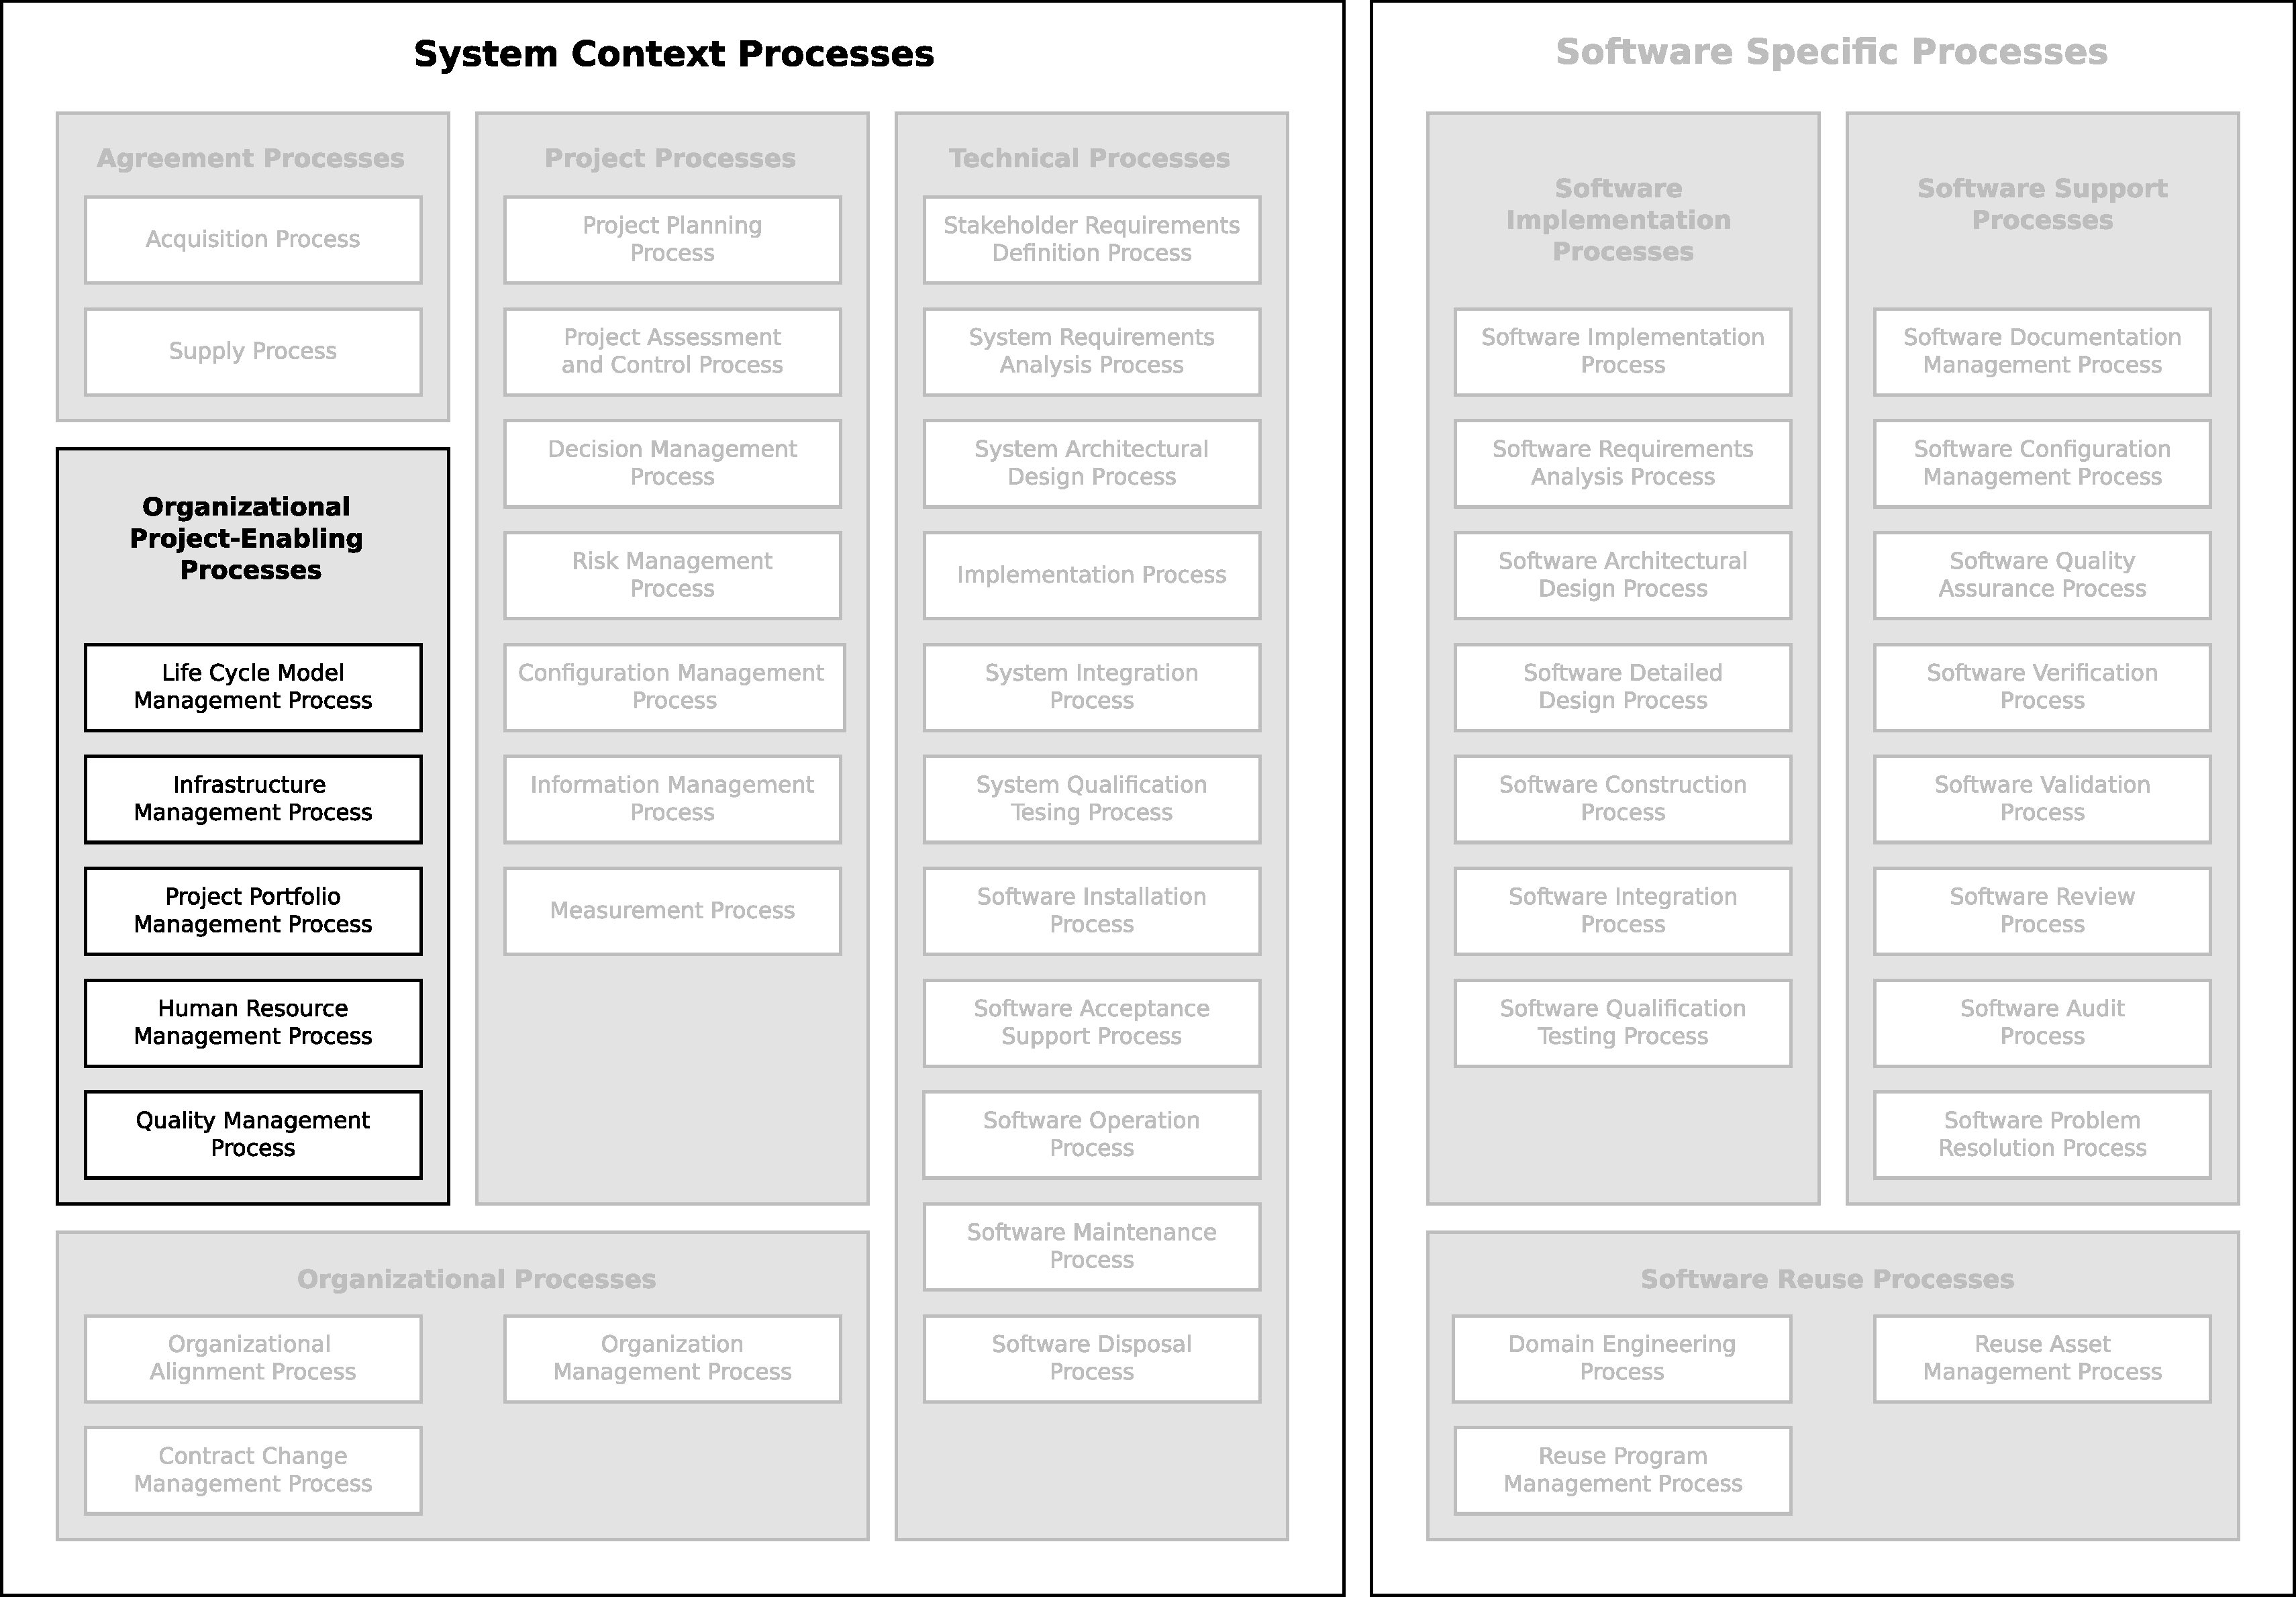
\includegraphics[width=15cm,keepaspectratio]{figures/life-cycle-process-groups-organizational-project-enabling-processes.pdf}
			\caption{Organizational Project-Enabling Processes}
			\label{fig:organizational_project_enabling_processes}
		\end{figure}

		\begin{adjustwidth}{1em}{0pt}

			The \nameref{subsec:organizational_project_enabling_processes} manage the organization's capability to acquire and supply products or services through the initiation, support and control of projects. 

			They provide resources and infrastructure necessary to support projects and ensure the satisfaction of organizational objectives and established agreements. They are not intended to be a comprehensive set of business processes that enable management of the organization's business.

			In this Section:

			\begin{compactitem}

				\item \ref{proc:life_cycle_model_management_process} - \nameref{proc:life_cycle_model_management_process}

				\item \ref{proc:infrastructure_management_process} - \nameref{proc:infrastructure_management_process}

				\item \ref{proc:project_portfolio_management_process} - \nameref{proc:project_portfolio_management_process}

				\item \ref{proc:human_resource_management_process} - \nameref{proc:human_resource_management_process}

				\item \ref{proc:quality_management_process} - \nameref{proc:quality_management_process}
			
			\end{compactitem}

		\end{adjustwidth}

		\newpage
		\subsubsection{LIFE CYCLE MODEL MANAGEMENT PROCESS\label{proc:life_cycle_model_management_process}}

			\subsubsubsection{PURPOSE}
			\begin{adjustwidth}{2em}{0pt} 

				The purpose of the Life Cycle Model Management Process is to define, maintain, and assure availability of policies, life cycle processes, life cycle models, and procedures for use by the organization with respect to the scope of this standard.

				This process provides life cycle policies, processes, and procedures that are consistent with the organization's objectives, that are defined, adapted, improved and maintained to support individual project needs within the context of the organization, and that are capable of being applied using effective, proven methods and tools.


			\end{adjustwidth}

			\subsubsubsection{OUTCOMES}
			\begin{adjustwidth}{2em}{0pt} 

				As a result of the successful implementation of the Life Cycle Model Management Process:

				\begin{compactitem}

					\item policies and procedures for the management and deployment of life cycle models and processes are provided;
					
					\item responsibility, accountability and authority for life cycle management are defined;
					
					\item life cycle processes, models and procedures for use by the organization are defined, maintained and improved; and
					
					\item prioritized process improvements are implemented.
				
				\end{compactitem}

			\end{adjustwidth}

			\subsubsubsection{ACTIVITIES AND TASKS}
			\begin{adjustwidth}{2em}{0pt} 

				\begin{compactenum}

					\item {\bf Process establishment}

					\begin{compactenum}

						\item The organization shall establish a suite of organizational processes for all software life cycle processes and life cycle models as they apply to its business activities. The processes and their application to specific cases shall be documented in the organization's publications. As appropriate, a process control mechanism should be established to develop, monitor, control, and improve the process(es).

					\end{compactenum}

					\item {\bf Process assessment}

					\begin{compactenum}

						\item The organization should develop, document and apply a process assessment procedure. Assessment records should be produced and maintained.

						\item The organization shall plan and carry out reviews of the processes at appropriate intervals to ensure their continuing suitability and effectiveness in the light of assessment results.

					\end{compactenum}

					\item {\bf Process improvement}

					\begin{compactenum}

						\item The organization shall effect such improvements to its processes as it determines to be necessary as a result of process assessment and review. Process documentation should be updated to reflect improvement in the organizational processes.
						
						\item Historical, technical, and evaluation data should be collected and analyzed to gain an understanding of the strengths and weaknesses of the employed processes. These analyses should be used as feedback to improve these processes, to recommend changes in the direction of the projects (or subsequent projects), and to determine technology advancement needs.

						\item Quality cost data should be collected, maintained, and used to improve the organization's processes as a management activity. These data shall serve the purpose of establishing the cost of both the prevention and resolution of problems and non-conformity in software products and services.
					
					\end{compactenum}

				\end{compactenum}

			\end{adjustwidth}
		
		\newpage
		\subsubsection{INFRASTRUCTURE MANAGEMENT PROCESS \label{proc:infrastructure_management_process}}

			\subsubsubsection{PURPOSE}
			\begin{adjustwidth}{2em}{0pt} 

				The purpose of the Infrastructure Management Process is to provide the enabling infrastructure and services to projects to support organization and project objectives throughout the life cycle.
				
				This process defines, provides and maintains the facilities, tools, and communications and information technology assets needed for the organization's business with respect to the scope of this standard.

			\end{adjustwidth}

			\subsubsubsection{OUTCOMES}
			\begin{adjustwidth}{2em}{0pt} 

				\begin{compactitem}

					\item The requirements for infrastructure to support processes are defined;

					\item The infrastructure elements are identified and specified;

					\item The infrastructure elements are implemented; and

					\item A stable and reliable infrastructure is maintained and improved.

				\end{compactitem}

				{\bf Note}: The infrastructure elements may include hardware, software, methods, tools, techniques, standards, and facilities for development, operation, or maintenance. 

			\end{adjustwidth}

			\subsubsubsection{ACTIVITIES AND TASKS}
			\begin{adjustwidth}{2em}{0pt} 

				The organization shall implement the following activities in accordance with applicable organization policies and procedures with respect to the \nameref{proc:infrastructure_management_process}.

				\begin{compactenum}

					\item {\bf Process implementation}:

					\begin{compactenum}
						
						\item The infrastructure should be defined and documented to meet the requirements of the process employing this process, considering the applicable procedures, standards, tools, and techniques.

						\item The establishment of the infrastructure should be planned and documented.

					\end{compactenum}

					\item {\bf Establishment of the infrastructure}:

					\begin{compactenum}
						
						\item The configuration of the infrastructure should be planned and documented. Functionality, performance, safety, security, availability, space requirements, equipment, costs, and time constraints should be considered.

						\item The infrastructure shall be installed in time for execution of the relevant process.

					\end{compactenum}

					\item {\bf Maintenance of the infrastructure}:

					\begin{compactenum}
						
						\item The infrastructure shall be maintained, monitored, and modified as necessary to ensure that it continues to satisfy the requirements of the process employing this process. As part of maintaining the infrastructure, the extent to which the infrastructure is under configuration management shall be defined.

					\end{compactenum}

				\end{compactenum}

			\end{adjustwidth}

		\newpage
		\subsubsection{PROJECT PORTFOLIO MANAGEMENT PROCESS\label{proc:project_portfolio_management_process}}

			\subsubsubsection{PURPOSE}
			\begin{adjustwidth}{2em}{0pt} 

				The purpose of the \nameref{proc:project_portfolio_management_process} is to initiate and sustain necessary, sufficient and suitable projects in order to meet the strategic objectives of the organization. 

				This process commits the investment of adequate organization funding and resources, and sanctions the authorities needed to establish selected projects. It performs continued qualification of projects to confirm they justify, or can be redirected to justify, continued investment.

			\end{adjustwidth}

			\subsubsubsection{OUTCOMES}
			\begin{adjustwidth}{2em}{0pt} 

				\begin{compactitem}

					\item Business venture opportunities, investments or necessities are qualified, prioritized and selected;

					\item Resources and budgets for each project are identified and allocated;

					\item Project management accountability and authorities are defined;

					\item Projects meeting agreement and stakeholder requirements are sustained; and

					\item projects not meeting agreement or stakeholder requirements are redirected or terminated.

				\end{compactitem}

			\end{adjustwidth}

			\subsubsubsection{ACTIVITIES AND TASKS}
			\begin{adjustwidth}{2em}{0pt} 
				
				The organization shall implement the following activities and tasks in accordance with applicable organization policies and procedures with respect to the \nameref{proc:project_portfolio_management_process}.

				\begin{compactenum}

					\item {\bf Project Initiation}:

					\begin{compactenum}

						\item The organization shall identify, prioritize, select, and establish new business opportunities, ventures, or undertakings in a manner that is consistent with the business strategy and action plans of the organization.

						\item The organization shall define accountabilities and authorities for each project.

						\item The organization shall identify the expected outcomes of the projects.

						\item The organization shall allocate resources for the achievement of project objectives.

						\item The organization shall identify any multi-project interfaces that must be managed or supported by the project.

						\item The organization shall specify the project reporting requirements and review milestones that will govern the execution of the project.
						
						\item The organization shall authorize the project to commence execution of approved project plans, including the technical plans.

					\end{compactenum}

					\item {\bf Project Evaluation}:

					\begin{compactenum}

						\item The organization shall evaluate ongoing projects to confirm that:

						\begin{compactenum}

							\item Projects are making progress towards achieving established goals.

							\item Projects are complying with project directives.

							\item Projects are being conducted according to system life cycle plans and procedures.

							\item Projects remain viable, as indicated by, for example, continuing need for the service, practicable product implementation, acceptable investment benefits.

						\end{compactenum}

						\item The organization shall act to continue or redirect projects that are satisfactorily progressing or can be expected to progress satisfactorily by appropriate redirection

					\end{compactenum}


					\item {\bf Project Closure}:

					\begin{compactenum}

						\item The organization shall act to cancel or suspend projects whose disadvantages or risks to the organization outweigh the benefits of continued investments, where agreements permit this.

						\item After completion of the agreement for products and services, the organization shall act to close the project per organizational policies and procedures and the agreement.

					\end{compactenum}

				\end{compactenum}

			\end{adjustwidth}

		\newpage
		\subsubsection{HUMAN RESOURCE MANAGEMENT PROCESS\label{proc:human_resource_management_process}}

			\subsubsubsection{PURPOSE}
			\begin{adjustwidth}{2em}{0pt} 
				
				The purpose of the \nameref{proc:human_resource_management_process} is to provide the organization with necessary human resources and to maintain their competencies, consistent with business needs. 

				The process assures the providing of a supply of skilled and experienced personnel qualified to perform life cycle processes to achieve organization, project and customer objectives.

			\end{adjustwidth}

			\subsubsubsection{OUTCOMES}
			\begin{adjustwidth}{2em}{0pt} 

				\begin{compactitem}

					\item skills required by projects are identified;

					\item necessary human resources are provided to projects;

					\item skills of personnel are developed, maintained or enhanced;

					\item conflicts in multi-project resource demands are resolved; and

					\item individual knowledge, information and skills are collected, shared, reused and improved throughout the organization.

				\end{compactitem}

			\end{adjustwidth}

			\subsubsubsection{ACTIVITIES AND TASKS}
			\begin{adjustwidth}{2em}{0pt} 

				\begin{compactenum}

					\item {\bf Skill Identification}

					\begin{compactenum}
						
						\item A review of the organization and project requirements shall be conducted to establish and make timely provision for acquiring or developing the resources and skills required by the management and technical staff. These needs may be met through training, recruitment or other staff development mechanisms.
						
						\item The types and levels of training and knowledge needed to satisfy organization and project requirements shall be determined.

					\end{compactenum}

					\item {\bf Skill Development}

					\begin{compactenum}
						
						\item A training plan, addressing implementation schedules, resource requirements, and training needs, should be developed and documented.

						\item Training manuals, including presentation materials used in providing training should be developed or acquired.
						
						\item The training plan shall be implemented to provide training to personnel. Training records should be maintained.

					\end{compactenum}

					\item {\bf Skill Acquisition and Provision}

					\begin{compactenum}
						
						\item Establish a systematic program for recruitment of staff qualified to meet the needs of the organization and projects. Provide opportunities for the career development of existing staff.

						\item Define objective criteria that can be used to evaluate staff performance.

						\item Evaluate the performance of the staff in respect of their contributions to the goals of the organization or project.

						\item Ensure that feedback is provided to the staff on the results of any evaluations performed.

						\item Maintain adequate records of staff performance including information on skills, training completed, and performance evaluations. 

						\item Define the organization's and project's need for project teams. Define team structure and operating rules.

						\item Conflicts in multi-project resource demands should be resolved.

						\item An understanding of their role on the project.

						\item A shared vision or sense of common interests on the success of the project.

						\item Appropriate mechanisms or facilities for communication and interactions among teams.

						\item Support from appropriate management to accomplish project requirements.

						\item It should be ensured that the right mix and categories of appropriately trained personnel are available for the planned activities and tasks in a timely manner.

					\end{compactenum}

					\item {\bf Knowledge Management}

					\begin{compactenum}	

						\item The organization shall plan the requirements for managing the organization's knowledge assets. The planning shall  include the definition of the infrastructure and training to support the contributors and the users of the organization's knowledge assets, the classification schema for the assets and the asset criteria.
						
						\item The organization shall establish a network of experts within the organization. The network shall contain the identification of the organization's experts, a list of their area of expertise and the identification of available information within a classification schema, e.g., knowledge area. The organization shall ensure that the network is maintained current.

						\item The organization shall establish a mechanism to support the exchange of information between the experts and the flow of expert information to the organization's projects. The mechanism shall support the organization's access, storage and retrieval requirements.

						\item The organization shall perform configuration management of assets in accordance with the \nameref{proc:configuration_management_process}.

						\item The organizations shall capture and maintain information for access by the organization per the plan.

					\end{compactenum}

				\end{compactenum}

			\end{adjustwidth}

		\newpage
		\subsubsection{QUALITY MANAGEMENT PROCESS\label{proc:quality_management_process}}

			\subsubsubsection{PURPOSE}
			\begin{adjustwidth}{2em}{0pt} 
				
				The purpose of the \nameref{proc:quality_management_process} is to assure that products, services and implementations of life cycle processes meet organizational quality objectives and achieve customer satisfaction.

			\end{adjustwidth}

			\subsubsubsection{OUTCOMES}
			\begin{adjustwidth}{2em}{0pt} 

				\begin{compactitem}

					\item organization quality management policies and procedures are defined;

					\item organization quality objectives are defined;

					\item accountability and authority for quality management are defined;

					\item the status of customer satisfaction is monitored; and

					\item appropriate action is taken when quality objectives are not achieved.

				\end{compactitem}

			\end{adjustwidth}

			\subsubsubsection{ACTIVITIES AND TASKS}
			\begin{adjustwidth}{2em}{0pt} 

				\begin{compactenum}

					\item {\bf Quality Management}

					\begin{compactenum}
						
						\item The organization shall establish quality management policies, standards and procedures.

						\item The organization shall establish organization quality management goals and objectives based on business strategy for customer satisfaction.
						
						\item The organization shall define responsibilities and authority for implementation of quality management.

						\item The organization shall assess customer satisfaction and report.

						\item The organization shall conduct periodic reviews of project quality plans.

						\item The organization shall monitor the status of quality improvements on products and services.

					\end{compactenum}


					\item {\bf Quality Management Corrective Action}

					\begin{compactenum}

						\item The organization shall take corrective actions when quality management goals are not
						
						\item The organization shall implement corrective actions and communicate results through the organization.

					\end{compactenum}

				\end{compactenum}

			\end{adjustwidth}


	\newpage 
	\subsection{PROJECT PROCESSES\label{subsec:project_processes}}

		\begin{figure}[h]
			\centering
			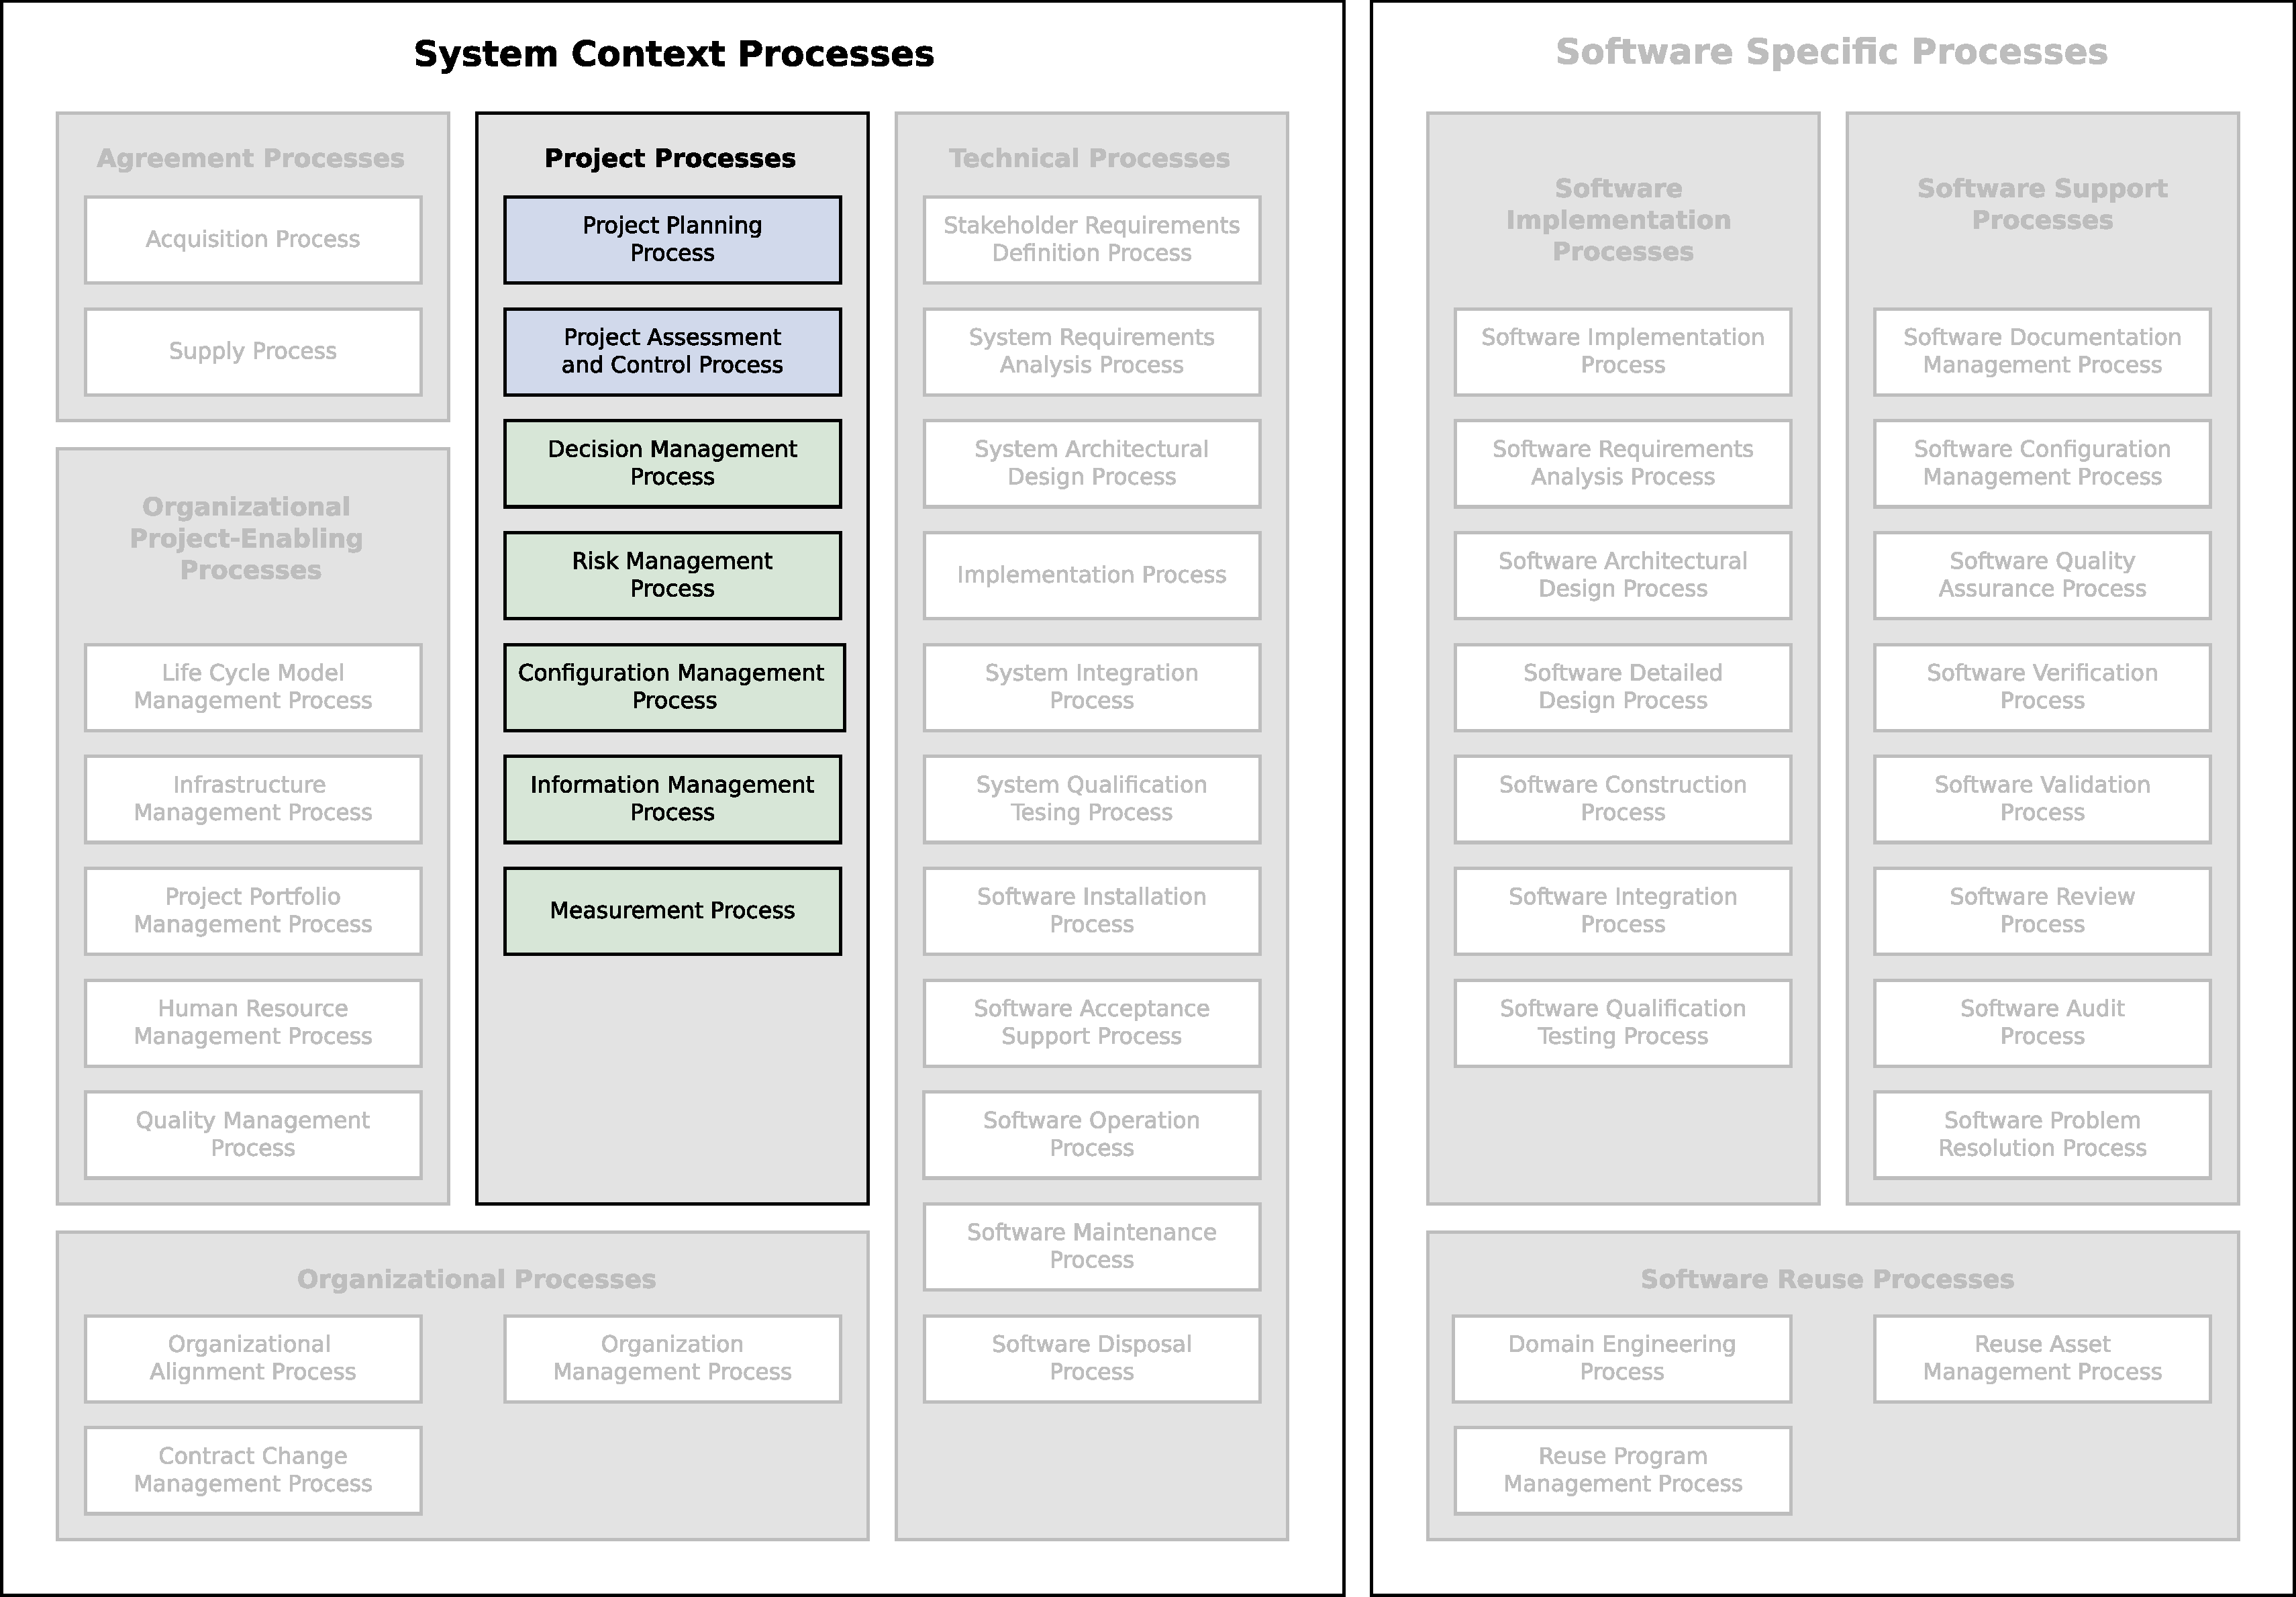
\includegraphics[width=15cm,keepaspectratio]{figures/life-cycle-process-groups-project-processes.pdf}
			\caption{Project Processes}
			\label{fig:project_processes}
		\end{figure}

		\begin{adjustwidth}{1em}{0pt}

			Within this standard, the project has been chosen as the context for describing processes concerned with planning, assessment and control. The principles related to these processes can be applied in any area of an organization's management.

			There are two categories of Project Processes. The Project Management Processes are used to plan, execute, assess and control the progress of a project. The Project Support Processes support specialized management objectives. Both are described below.
			
			The Project Management Processes are used to establish and evolve project plans, to assess actual achievement and progress against the plans and to control execution of the project through to fulfillment. Individual Project Management Processes may be invoked at any time in the life cycle and at any level in a hierarchy of projects, as required by project plans or unforeseen events. The Project Management Processes are applied with a level of rigor and formality that depends on the risk and complexity of the project.

			The Project Support Processes provide a specific focused set of tasks for performing a specialized management objective. They are all evident in the management of any undertaking, ranging from a complete organization down to a single life cycle process and its tasks.

		\end{adjustwidth}
		
		\newpage
		\subsubsection{PROJECT PLANNING PROCESS\label{proc:project_planning_process}}

			\subsubsubsection{PURPOSE}
			\begin{adjustwidth}{2em}{0pt}

				The purpose of the \nameref{proc:project_planning_process} is to produce and communicate effective and workable project plans.

				This process determines the scope of the project management and technical activities, identifies process outputs, project tasks and deliverables, establishes schedules for project task conduct, including achievement criteria, and required resources to accomplish project tasks.

			\end{adjustwidth}

			\subsubsubsection{OUTCOMES}
			\begin{adjustwidth}{2em}{0pt}

				\begin{compactitem}
					\item The scope of the work for the project is defined;
					\item The feasibility of achieving the goals of the project with available resources and constraints are evaluated;
					\item The tasks and resources necessary to complete the work are sized and estimated;
					\item Interfaces between elements in the project, and with other project and organizational units, are identified;
					\item Plans for the execution of the project are developed; and
					\item Plans for the execution of the project are activated.
				\end{compactitem}
			
			\end{adjustwidth}

			\subsubsubsection{ACTIVITIES AND TASKS}
			\begin{adjustwidth}{2em}{0pt}

				\begin{compactenum}

					\item {\bf Project initiation}:
					\begin{compactenum}
						\item The manager shall establish the requirements of the project to be undertaken.

						\item Once the project requirements are established, the manager shall establish the feasibility of the project by checking that the resources (personnel, materials, technology, and environment) required to execute and manage the project are available, adequate, and appropriate and that the timescales to completion are achievable.

						\item As necessary, and by agreement of all parties concerned, the requirements of the project may be modified at this point to achieve the completion criteria.
					\end{compactenum}

					\item {\bf Project planning}:
					\begin{compactenum}
						\item The manager shall prepare the plans for execution of the project. The plans associated with the execution of the project shall contain descriptions of the associated activities and tasks and identification of the software products that will be provided. These plans shall include, but are not limited to, the following:

						\begin{compactenum}
							\item Schedules for the timely completion of tasks.
							\item Estimation of effort.
							\item Adequate resources needed to execute the tasks.
							\item Allocation of tasks.
							\item Assignment of responsibilities.
							\item Quantification of risks associated with the tasks or the process itself.
							\item Quality assurance measures to be employed throughout the project.
							\item Costs associated with the process execution.
							\item Provision of environment and infrastructure.
							\item Definition and maintenance of a life cycle model that is comprised of stages using the defined life cycle models for projects of the organization
						\end{compactenum}

					\end{compactenum}

					\item {\bf Project activation}:
					\begin{compactenum}
						\item The manager shall obtain authorization for the project.

						\item The manager shall submit requests for necessary resources to perform the project.

						\item The manager shall initiate the implementation of the project plan/s to satisfy the objectives and criteria set, exercising control over the project
					\end{compactenum}

				\end{compactenum}

			\end{adjustwidth}

		\newpage
		\subsubsection{PROJECT ASSESSMENT AND CONTROL PROCESS\label{proc:project_assessment_and_control_process}}

			\subsubsubsection{PURPOSE}
			\begin{adjustwidth}{2em}{0pt}

				The purpose of the \nameref{proc:project_assessment_and_control_process} is to determine the status of the project and ensure that the project performs according to plans and schedules, and within projected budgets, and that it satisfies technical objectives. 

				This process includes redirecting the project activities, as appropriate, to correct identified deviations and variations from other project management or technical processes. Redirection may include replanning as appropriate.
			
			\end{adjustwidth}

			\subsubsubsection{OUTCOMES}
			\begin{adjustwidth}{2em}{0pt}

				\begin{compactitem}

					\item progress of the project is monitored and reported;

					\item interfaces between elements in the project, and with other project and organizational units, are monitored;

					\item actions to correct deviations from the plan and to prevent recurrence of problems identified in the project are taken when project targets are not achieved; and

					\item project objectives are achieved and recorded.

				\end{compactitem}

			\end{adjustwidth}

			\subsubsubsection{ACTIVITIES AND TASKS}
			\begin{adjustwidth}{2em}{0pt} 

				\begin{compactenum}

					\item {\bf Project Monitoring}

					\begin{compactenum}

						\item The manager shall monitor the overall execution of the project, providing both internal reporting of the project progress and external reporting to the acquirer as defined in the contract.

					\end{compactenum}


					\item {\bf Project Control}

					\begin{compactenum}
						
						\item The manager shall investigate, analyze, and resolve the problems discovered during the execution of the project. The resolution of problems may result in changes to plans. It is the manager's responsibility to ensure the impact of any changes is determined, controlled, and monitored. Problems and their resolution shall be documented.

						\item The manager shall report, at agreed points, the progress of the project, declaring adherence to the plans and resolving instances of the lack of progress. These include internal and external reporting as required by the organizational procedures and the contract.

					\end{compactenum}

					\item {\bf Project Assessment}

					\begin{compactenum}

						\item The manager shall ensure that the software products and plans are evaluated for satisfaction of requirements.

						\item The manager shall assess the evaluation results of the software products, activities, and tasks completed during the execution of the project for achievement of the objectives and completion of the plans.

					\end{compactenum}


					\item {\bf Project Closure}

					\begin{compactenum}

						\item When all software products, activities, and tasks are completed, the manager shall determine whether the project is complete, taking into account the criteria as specified in the contract or as part of organization's procedure.

						\item These results and records shall be archived in a suitable environment as specified in the contract.

					\end{compactenum}

				\end{compactenum}

			\end{adjustwidth}

		\newpage
		\subsubsection{DECISION MANAGEMENT PROCESS\label{proc:decision_management_process}}

			\subsubsubsection{PURPOSE}
			\begin{adjustwidth}{2em}{0pt} 

				The purpose of the \nameref{proc:decision_management_process} is to select the most beneficial course of project action where alternatives exist.

				This process responds to a request for a decision encountered during the system life cycle, whatever its nature or source, in order to reach specified, desirable or optimized outcomes. Alternative actions are analyzed and a course of action selected and directed. Decisions and their rationale are recorded to support future decision-making.

			\end{adjustwidth}

			\subsubsubsection{OUTCOMES}
			\begin{adjustwidth}{2em}{0pt} 

				\begin{compactitem}

					\item a decision-making strategy is defined;

					\item alternative courses of action are defined;

					\item a preferred course of action is selected; and

					\item the resolution, decision rationale and assumptions are captured and reported. 

				\end{compactitem}

			\end{adjustwidth}

			\subsubsubsection{ACTIVITIES AND TASKS}
			\begin{adjustwidth}{2em}{0pt} 

				\begin{compactenum}

					\item {\bf Decision Planning}:
					\begin{compactenum}

						\item The project shall involve relevant parties in the decision-making in order to draw on experience and knowledge.

						\item The project shall identify the circumstances and need for a decision.

					\end{compactenum}

					\item {\bf Decision Analysis}:
					\begin{compactenum}

						\item The project shall select and declare the decision-making strategy for each decision situation. 

						\item The project shall identify desired outcomes and measurable success criteria.
						
						\item The project shall evaluate the balance of consequences of alternative actions, using the defined decision-making strategy, to arrive at an optimization of, or an improvement in, an identified decision situation.

					\end{compactenum}

					\item {\bf Decision Tracking}:
					\begin{compactenum}

						\item The project shall record, track, evaluate and report decision outcomes to confirm that problems have been effectively resolved, adverse trends have been reversed and advantage has been taken of opportunities.

						\item The project shall maintain records of problems and opportunities and their disposition, as stipulated in agreements or organizational procedures and in a manner that permits auditing and learning from experience.
						
					\end{compactenum}

				\end{compactenum}

			\end{adjustwidth}

		\newpage
		\subsubsection{RISK MANAGEMENT PROCESS\label{proc:risk_management_process}}

			\subsubsubsection{PURPOSE}
			\begin{adjustwidth}{2em}{0pt} 
				
				The purpose of the \nameref{proc:risk_management_process} is to identify, analyze, treat and monitor the risks continuously.

				The Risk Management Process is a continuous process for systematically addressing risk throughout the life cycle of a system or software product or service. It can be applied to risks related to the acquisition, development, maintenance or operation of a system.

			\end{adjustwidth}

			\subsubsubsection{OUTCOMES}
			\begin{adjustwidth}{2em}{0pt} 

				\begin{compactitem}

					\item the scope of risk management to be performed is determined;

					\item appropriate risk management strategies are defined and implemented;

					\item risks are identified as they develop and during the conduct of the project;

					\item risks are analyzed, and the priority in which to apply resources to treatment of these risks is determined;

					\item risk measures are defined, applied, and assessed to determine changes in the status of risk and the progress of the treatment activities; and

					\item appropriate treatment is taken to correct or avoid the impact of risk based on its priority, probability, and consequence or other defined risk threshold.

				\end{compactitem}

			\end{adjustwidth}

			\subsubsubsection{ACTIVITIES AND TASKS}
			\begin{adjustwidth}{2em}{0pt} 

				\begin{compactenum}

					\item {\bf Risk Management Planning}:

					\begin{compactenum}
						\item Risk management policies describing the guidelines under which risk management is to be performed shall be defined.

						\item A description of the Risk Management Process to be implemented shall be documented.

						\item The parties responsible for performing risk management and their roles and responsibilities shall be identified.

						\item The responsible parties shall be provided with adequate resources to perform the Risk Management Process.

						\item A description of the process for evaluating and improving the Risk Management Process shall be provided.
					\end{compactenum}

					\item {\bf Risk Profile Management}:

					\begin{compactenum}
						\item Risk thresholds, defining the conditions under which a level of risk may be accepted, shall be documented.

						\item A risk profile shall be established and maintained.

						\item The relevant risk profile shall be communicated periodically to stakeholders based upon their needs.
					\end{compactenum}

					\item {\bf Risk Analysis}:

					\begin{compactenum}
						\item Risks shall be identified in the categories described in the risk management context.

						\item The probability of occurrence and consequences of each risk identified shall be estimated.

						\item Each risk shall be evaluated against its risk thresholds.

						\item For each risk that is above its risk threshold, recommended treatment strategies shall be defined and documented. Measures indicating the effectiveness of the treatment alternatives shall also be defined and documented.

						\item Stakeholders shall be provided recommended alternatives for risk treatment in risk action requests.
					\end{compactenum}

					\item {\bf Risk Treatment}:

					\begin{compactenum}
						\item If the stakeholders determine that actions should be taken to make a risk acceptable, then a risk treatment alternative shall be implemented.

						\item If the stakeholders accept a risk that exceeds its threshold, it shall be considered a high priority and monitored continuously to determine if any future risk treatment actions are necessary.

						\item Once a risk treatment is selected, it shall receive the same management actions as problems do, in accordance with the assessment and control activities in the \nameref{proc:project_assessment_and_control_process}.
					\end{compactenum}

					\item {\bf Risk Monitoring}:

					\begin{compactenum}
						\item All risks and the risk management context shall be continuously monitored for changes. Risks whose states have changed shall undergo risk evaluation.

						\item Measures shall be implemented and monitored to evaluate the effectiveness of risk treatments.

						\item The project shall continuously monitor for new risks and sources throughout its life cycle.
					\end{compactenum}

					\item {\bf Risk Management Process Evaluation}:

					\begin{compactenum}
						\item Information shall be collected throughout the project's life cycle for purposes of improving the Risk Management Process and generating lessons learned.

						\item The Risk Management Process shall be periodically reviewed for its effectiveness and efficiency.

						\item Information on the risks identified, their treatment, and the success of the treatments shall be reviewed periodically for purposes of identifying systemic project and organizational risks.
					\end{compactenum}

				\end{compactenum}

			\end{adjustwidth}

		\newpage
		\subsubsection{CONFIGURATION MANAGEMENT PROCESS\label{proc:configuration_management_process}}

			\subsubsubsection{PURPOSE}
			\begin{adjustwidth}{2em}{0pt} 

				The purpose of the \nameref{proc:configuration_management_process} is to establish and maintain the integrity of all identified outputs of a project or process and make them available to concerned parties.

			\end{adjustwidth}

			\subsubsubsection{OUTCOMES}
			\begin{adjustwidth}{2em}{0pt} 

				\begin{compactitem}

					\item a configuration management strategy is defined;

					\item items requiring configuration management are defined;

					\item configuration baselines are established;

					\item changes to items under configuration management are controlled;

					\item the configuration of released items is controlled; and

					\item the status of items under configuration management is made available throughout the life cycle.

				\end{compactitem}

			\end{adjustwidth}

			\subsubsubsection{ACTIVITIES AND TASKS}
			\begin{adjustwidth}{2em}{0pt} 

				\begin{compactenum}

					\item {\bf Configuration Management Planning}:

					\begin{compactenum}

						\item The project shall define a configuration management strategy.

						\item The project shall identify items that are subject to configuration control.

					\end{compactenum}

					\item {\bf Configuration Management Execution}:

					\begin{compactenum}

						\item The project shall maintain information on configurations with an appropriate level of integrity and security.

						\item The project shall ensure that changes to configuration baselines are properly identified, recorded, evaluated, approved, incorporated and verified.

					\end{compactenum}

				\end{compactenum}

			\end{adjustwidth}

		\newpage
		\subsubsection{INFORMATION MANAGEMENT PROCESS\label{proc:information_management_process}}

			\subsubsubsection{PURPOSE}
			\begin{adjustwidth}{2em}{0pt} 

				The purpose of the \nameref{proc:information_management_process} is to provide relevant, timely, complete, valid and, if required, confidential information to designated parties during and, as appropriate, after the system life cycle.

				This process generates, collects, transforms, retains, retrieves, disseminates and disposes of information. It manages designated information, including technical, project, organizational, agreement and user information.

			\end{adjustwidth}

			\subsubsubsection{OUTCOMES}
			\begin{adjustwidth}{2em}{0pt} 

				\begin{compactitem}

					\item information to be managed is identified;

					\item the forms of the information representations are defined;

					\item information is transformed and disposed of as required;

					\item the status of information is recorded;

					\item information is current, complete and valid; and

					\item information is made available to designated parties.

				\end{compactitem}

			\end{adjustwidth}

			\subsubsubsection{ACTIVITIES AND TASKS}
			\begin{adjustwidth}{2em}{0pt} 

				\begin{compactenum}

					\item {\bf Information Management Planning}:

					\begin{compactenum}

						\item The project shall define the items of information that will be managed during the system life cycle and, according to organizational policy or legislation, maintained for a defined period beyond.

						\item The project shall designate authorities and responsibilities regarding the origination, generation, capture, archiving and disposal of items of information.

						\item The project shall define the rights, obligations and commitments regarding the retention of, transmission of and access to information items.

						\item The project shall define the content, semantics, formats and medium for the representation, retention, transmission and retrieval of information.

						\item  The project shall define information maintenance actions. 

					\end{compactenum}

					\item {\bf Information Management Execution}:

					\begin{compactenum}

						\item The project shall obtain the identified items of information.

						\item The project shall maintain information items and their storage records according to integrity, security and privacy requirements.

						\item The project shall retrieve and distribute information to designated parties as required by agreed schedules or defined circumstances.

						\item The project shall provide official documentation as required.

						\item The project shall archive designated information, in accordance with the audit, knowledge retention and project closure purposes.

						\item The project shall dispose of unwanted, invalid or unverifiable information according to organization policy, and security and privacy requirements.

					\end{compactenum}

				\end{compactenum}

			\end{adjustwidth}

		\newpage
		\subsubsection{MEASUREMENT PROCESS\label{proc:measurement_process}}

			\subsubsubsection{PURPOSE}
			\begin{adjustwidth}{2em}{0pt} 

				The purpose of the \nameref{proc:measurement_process} is to collect, analyze, and report data relating to the products developed and processes implemented within the organizational unit, to support effective management of the processes, and to objectively demonstrate the quality of the products.

			\end{adjustwidth}

			\subsubsubsection{OUTCOMES}
			\begin{adjustwidth}{2em}{0pt} 

				\begin{compactitem}

					\item the information needs of technical and management processes are identified;

					\item an appropriate set of measures, driven by the information needs are identified and/or developed;

					\item measurement activities are identified and planned;

					\item the required data are collected, stored, analyzed, and the results interpreted;

					\item information products are used to support decisions and provide an objective basis for communication;

					\item the Measurement Process and measures are evaluated; and

					\item improvements are communicated to the Measurement Process owner.

				\end{compactitem}

			\end{adjustwidth}

			\subsubsubsection{ACTIVITIES AND TASKS}
			\begin{adjustwidth}{2em}{0pt} 

				\begin{compactenum}

					\item {\bf Measurement Planning}:

					\begin{compactenum}

						\item The project shall describe the characteristics of the organization that are relevant to measurement.

						\item The project shall identify and prioritize the information needs.

						\item The project shall select and document measures that satisfy the information needs.

						\item The project shall define data collection, analysis, and reporting procedures.

						\item The project shall define criteria for evaluating the information products and the measurement process.

						\item The project shall review, approve, and provide resources for measurement tasks.

						\item The project shall acquire and deploy supporting technologies.

					\end{compactenum}

					\item {\bf Measurement Performance}:

					\begin{compactenum}

						\item The project shall integrate procedures for data generation, collection, analysis and reporting into the relevant processes.

						\item The project shall collect, store, and verify data.

						\item The project shall analyze data and develop information products.

						\item The project shall document and communicate results to the measurement users.

					\end{compactenum}

					\item {\bf Measurement Evaluation}:

					\begin{compactenum}

						\item The project shall evaluate information products and the measurement process.

						\item The project shall identify and communicate potential improvements.

					\end{compactenum}

				\end{compactenum}

			\end{adjustwidth}


	\newpage 
	\subsection{ORGANIZATIONAL PROCESSES\label{subsec:organizational_processes}}

		\begin{figure}[h]
			\centering
			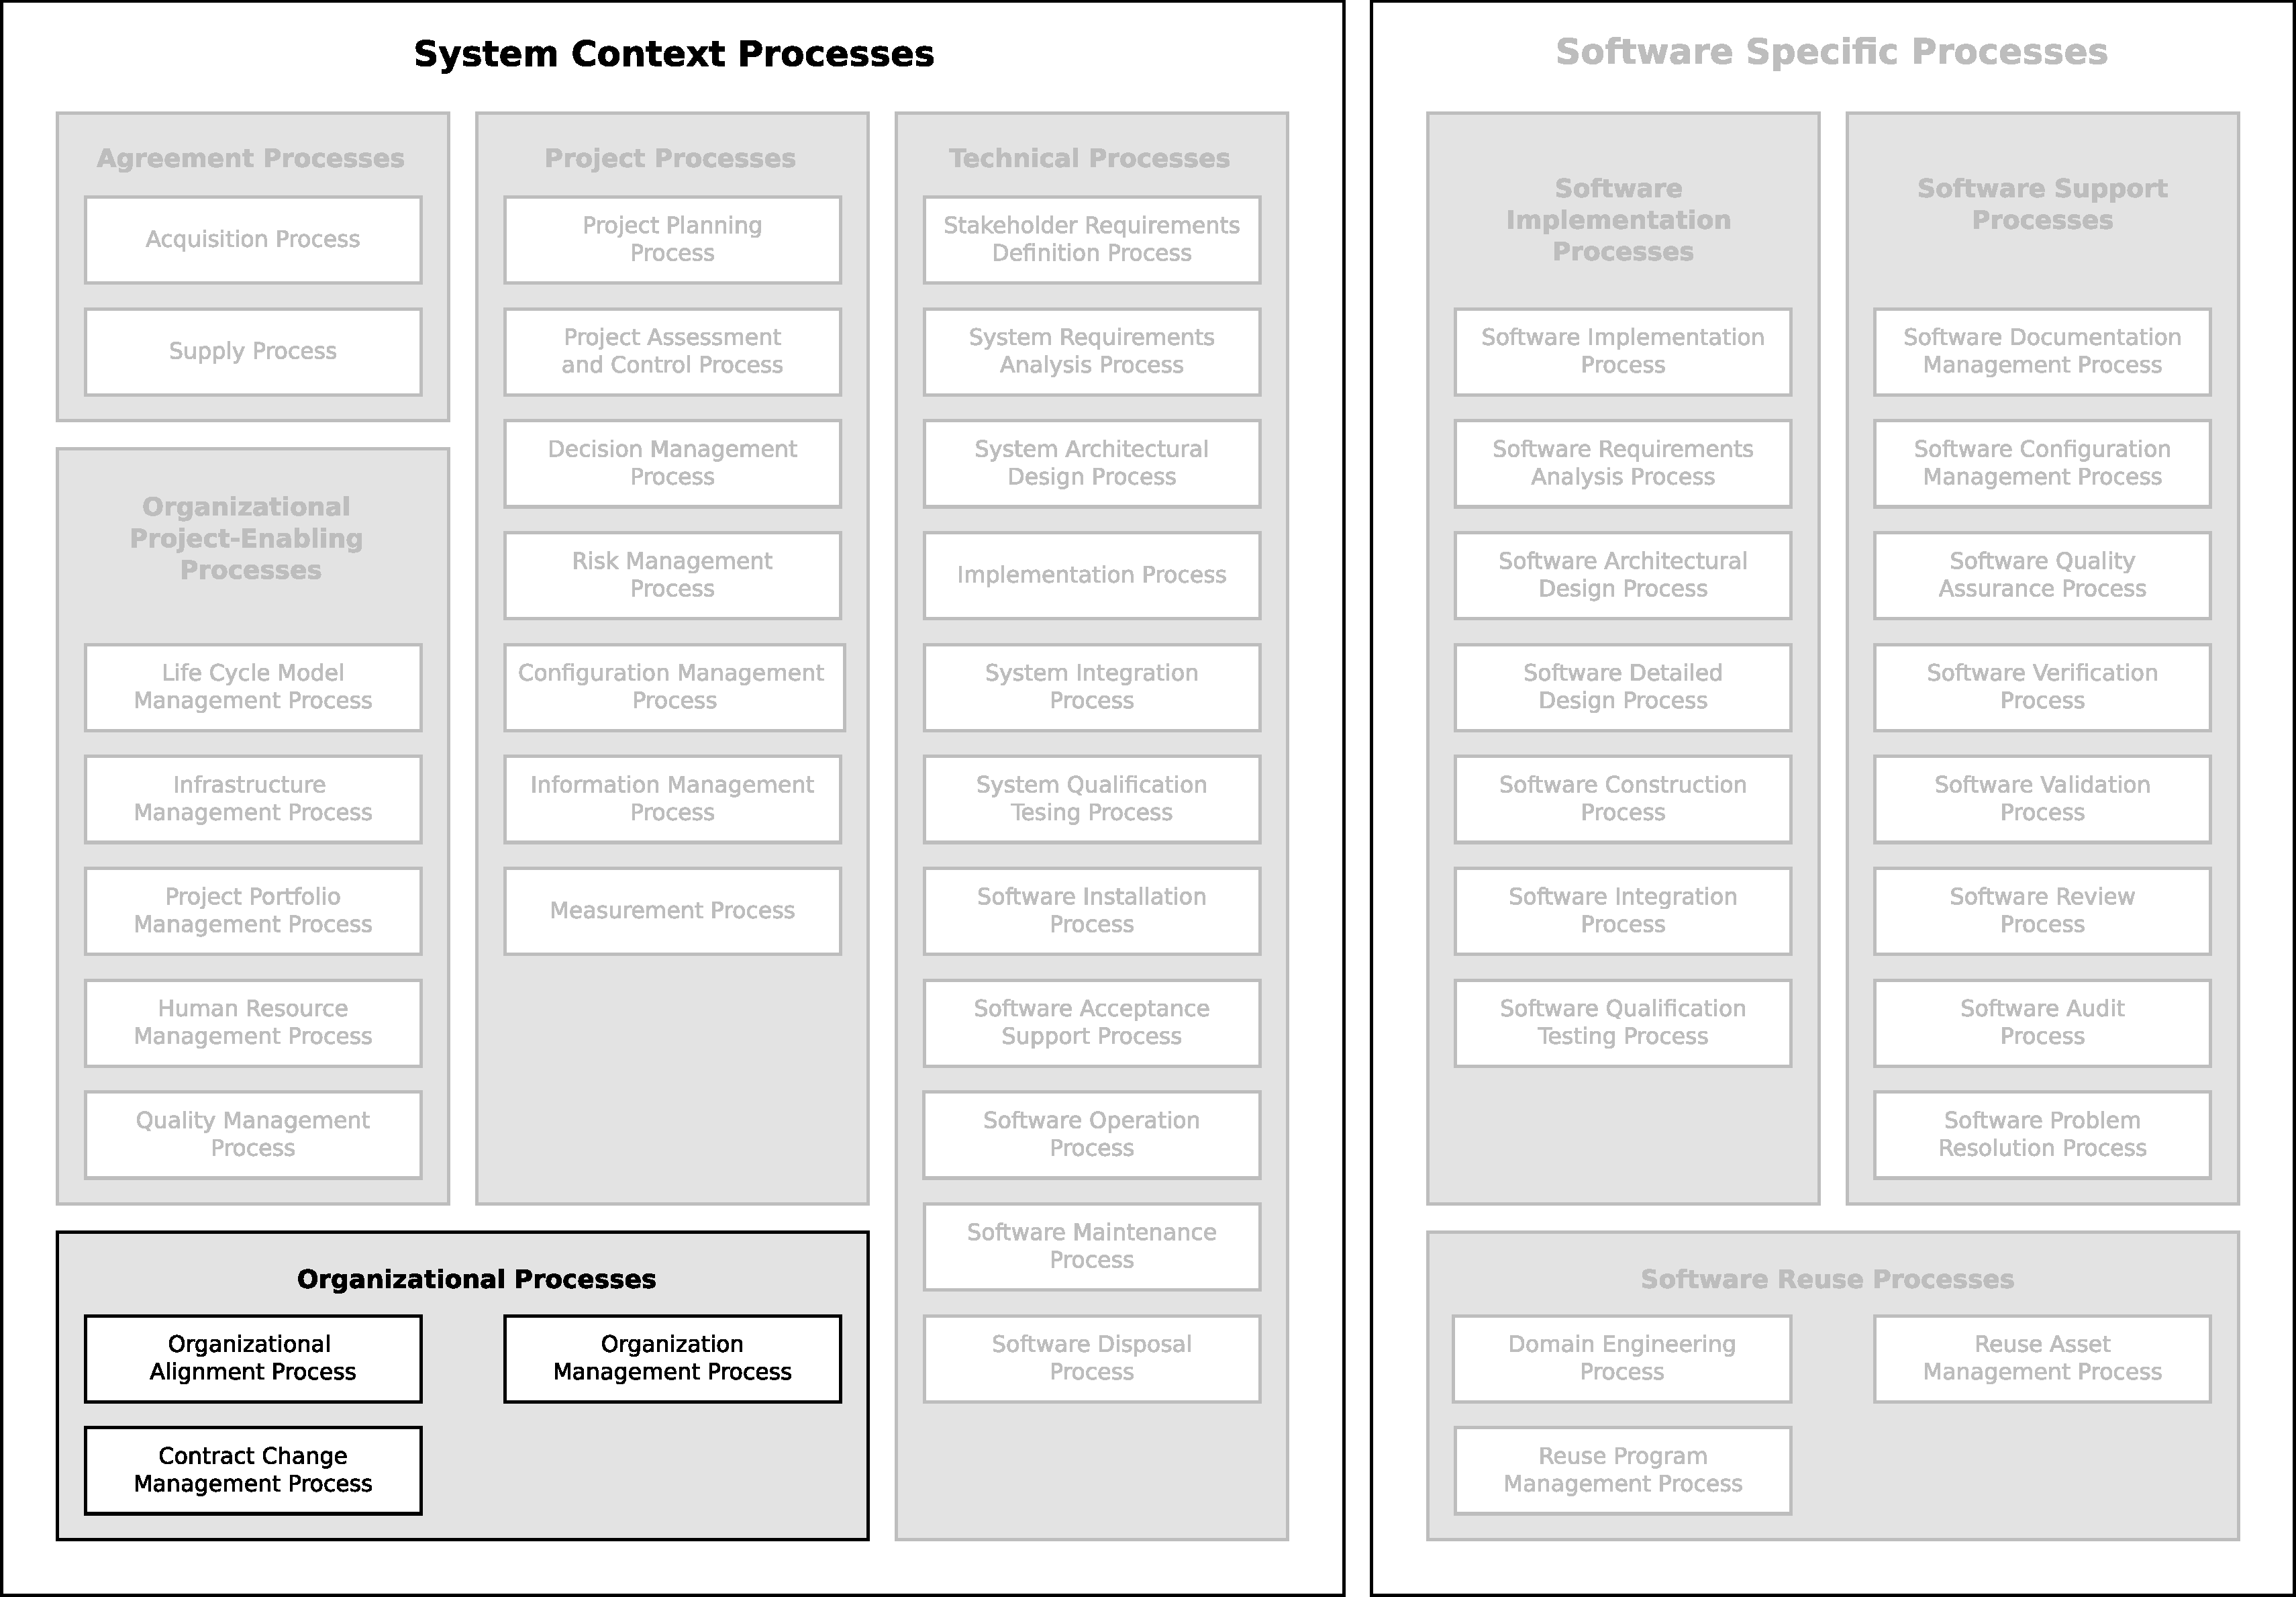
\includegraphics[width=15cm,keepaspectratio]{figures/life-cycle-process-groups-organizational-processes.pdf}
			\caption{Organizational Processes}
			\label{fig:organizational_processes}
		\end{figure}

		\begin{adjustwidth}{1em}{0pt}

			The processes within this section are considered highly useful to the management of an organization and its use and management of the processes within this standard.

			In this Section:

			\begin{compactitem}
			
				\item \ref{proc:organizational_alignment_process} - \nameref{proc:organizational_alignment_process}

				\item \ref{proc:organization_management_process} - \nameref{proc:organization_management_process}

				\item \ref{proc:contract_change_management_process} - \nameref{proc:contract_change_management_process}
			
			\end{compactitem}

		\end{adjustwidth}

		\newpage
		\subsubsection{ORGANIZATIONAL ALIGNMENT PROCESS\label{proc:organizational_alignment_process}}
		
			\subsubsubsection{PURPOSE}
			\begin{adjustwidth}{2em}{0pt}

				The purpose of the \nameref{proc:organizational_alignment_process} is to enable the software processes needed by the organization to provided software products and services, to be consistent with its goals. Within this context, goals are defined by the business' highest-order business objectives. 

			\end{adjustwidth}

			\subsubsubsection{OUTCOMES}
			\begin{adjustwidth}{2em}{0pt}

				\begin{compactitem}

					\item The organization's business goals are identified;

					\item The process framework is identified and defined that includes a set of software processes needed to achieve the business goals of the organization;
					
					\item A strategy is defined for process definition, implementation and improvement;
					
					\item Support is provided to enable this strategy;
					
					\item The organization's mission, core values, vision, goals and objectives is made known to all employees;
					
					\item Individuals in the organization share a common vision, culture, and understanding of the business goals to empower them to function effectively; and
					
					\item Everyone in the organization understands their role in achieving the goals of the business and is able to perform that role.
				
				\end{compactitem}

			\end{adjustwidth}

		\newpage
		\subsubsection{ORGANIZATION MANAGEMENT PROCESS\label{proc:organization_management_process}}

			\subsubsubsection{PURPOSE}
			\begin{adjustwidth}{2em}{0pt} 

				The purpose of the \nameref{proc:organization_management_process} is to establish and perform software management practices, during the performance of the processes needed for providing software products and services, that are consistent with the business goals of the organization.

				{\bf Note}: Although organizational operations in general have a much broader scope than that of software process, software processes are implemented in a business context and to be effective, require an appropriate organizational environment.

			\end{adjustwidth}

			\subsubsubsection{OUTCOMES}
			\begin{adjustwidth}{2em}{0pt} 

				\begin{compactitem}

					\item the organization will invest in the appropriate management infrastructure;

					\item the best practices are identified to support the implementation of effective organization and project management; and

					\item a basis for evaluating the achievement of organization business goals based on these management practices is provided.

				\end{compactitem}

			\end{adjustwidth}

		\newpage
		\subsubsection{CONTRACT CHANGE MANAGEMENT PROCESS\label{proc:contract_change_management_process}}

			\subsubsubsection{PURPOSE}
			\begin{adjustwidth}{2em}{0pt} 

				The purpose of the \nameref{proc:contract_change_management_process} is to develop the new contract contents as agreed by both the acquirer and the supplier when a change request affecting the agreed contract contents is proposed. 

				This process begins with a proposal of the change request by either the acquirer or the supplier and ends with the conclusion acceptable for both parties: withdrawal or overall/partial approval of the change request.

			\end{adjustwidth}

			\subsubsubsection{OUTCOMES}
			\begin{adjustwidth}{2em}{0pt} 

				\begin{compactitem}

					\item the change request to the contract is proposed explicitly and formally;

					\item the roles and responsibilities of both the acquirer and the supplier for the contract change management are established;

					\item the impact of the change request to the contract on the project plans, costs, benefits, quality and schedule is evaluated;

					\item the actions against the change request are taken to get agreement and satisfaction of both the acquirer and the supplier; and

					\item the result of each change request is made known to all affected parties.

				\end{compactitem}

			\end{adjustwidth}


	\newpage 
	\subsection{TECHNICAL PROCESSES\label{subsec:technical_processes}}

		\begin{figure}[h]
			\centering
			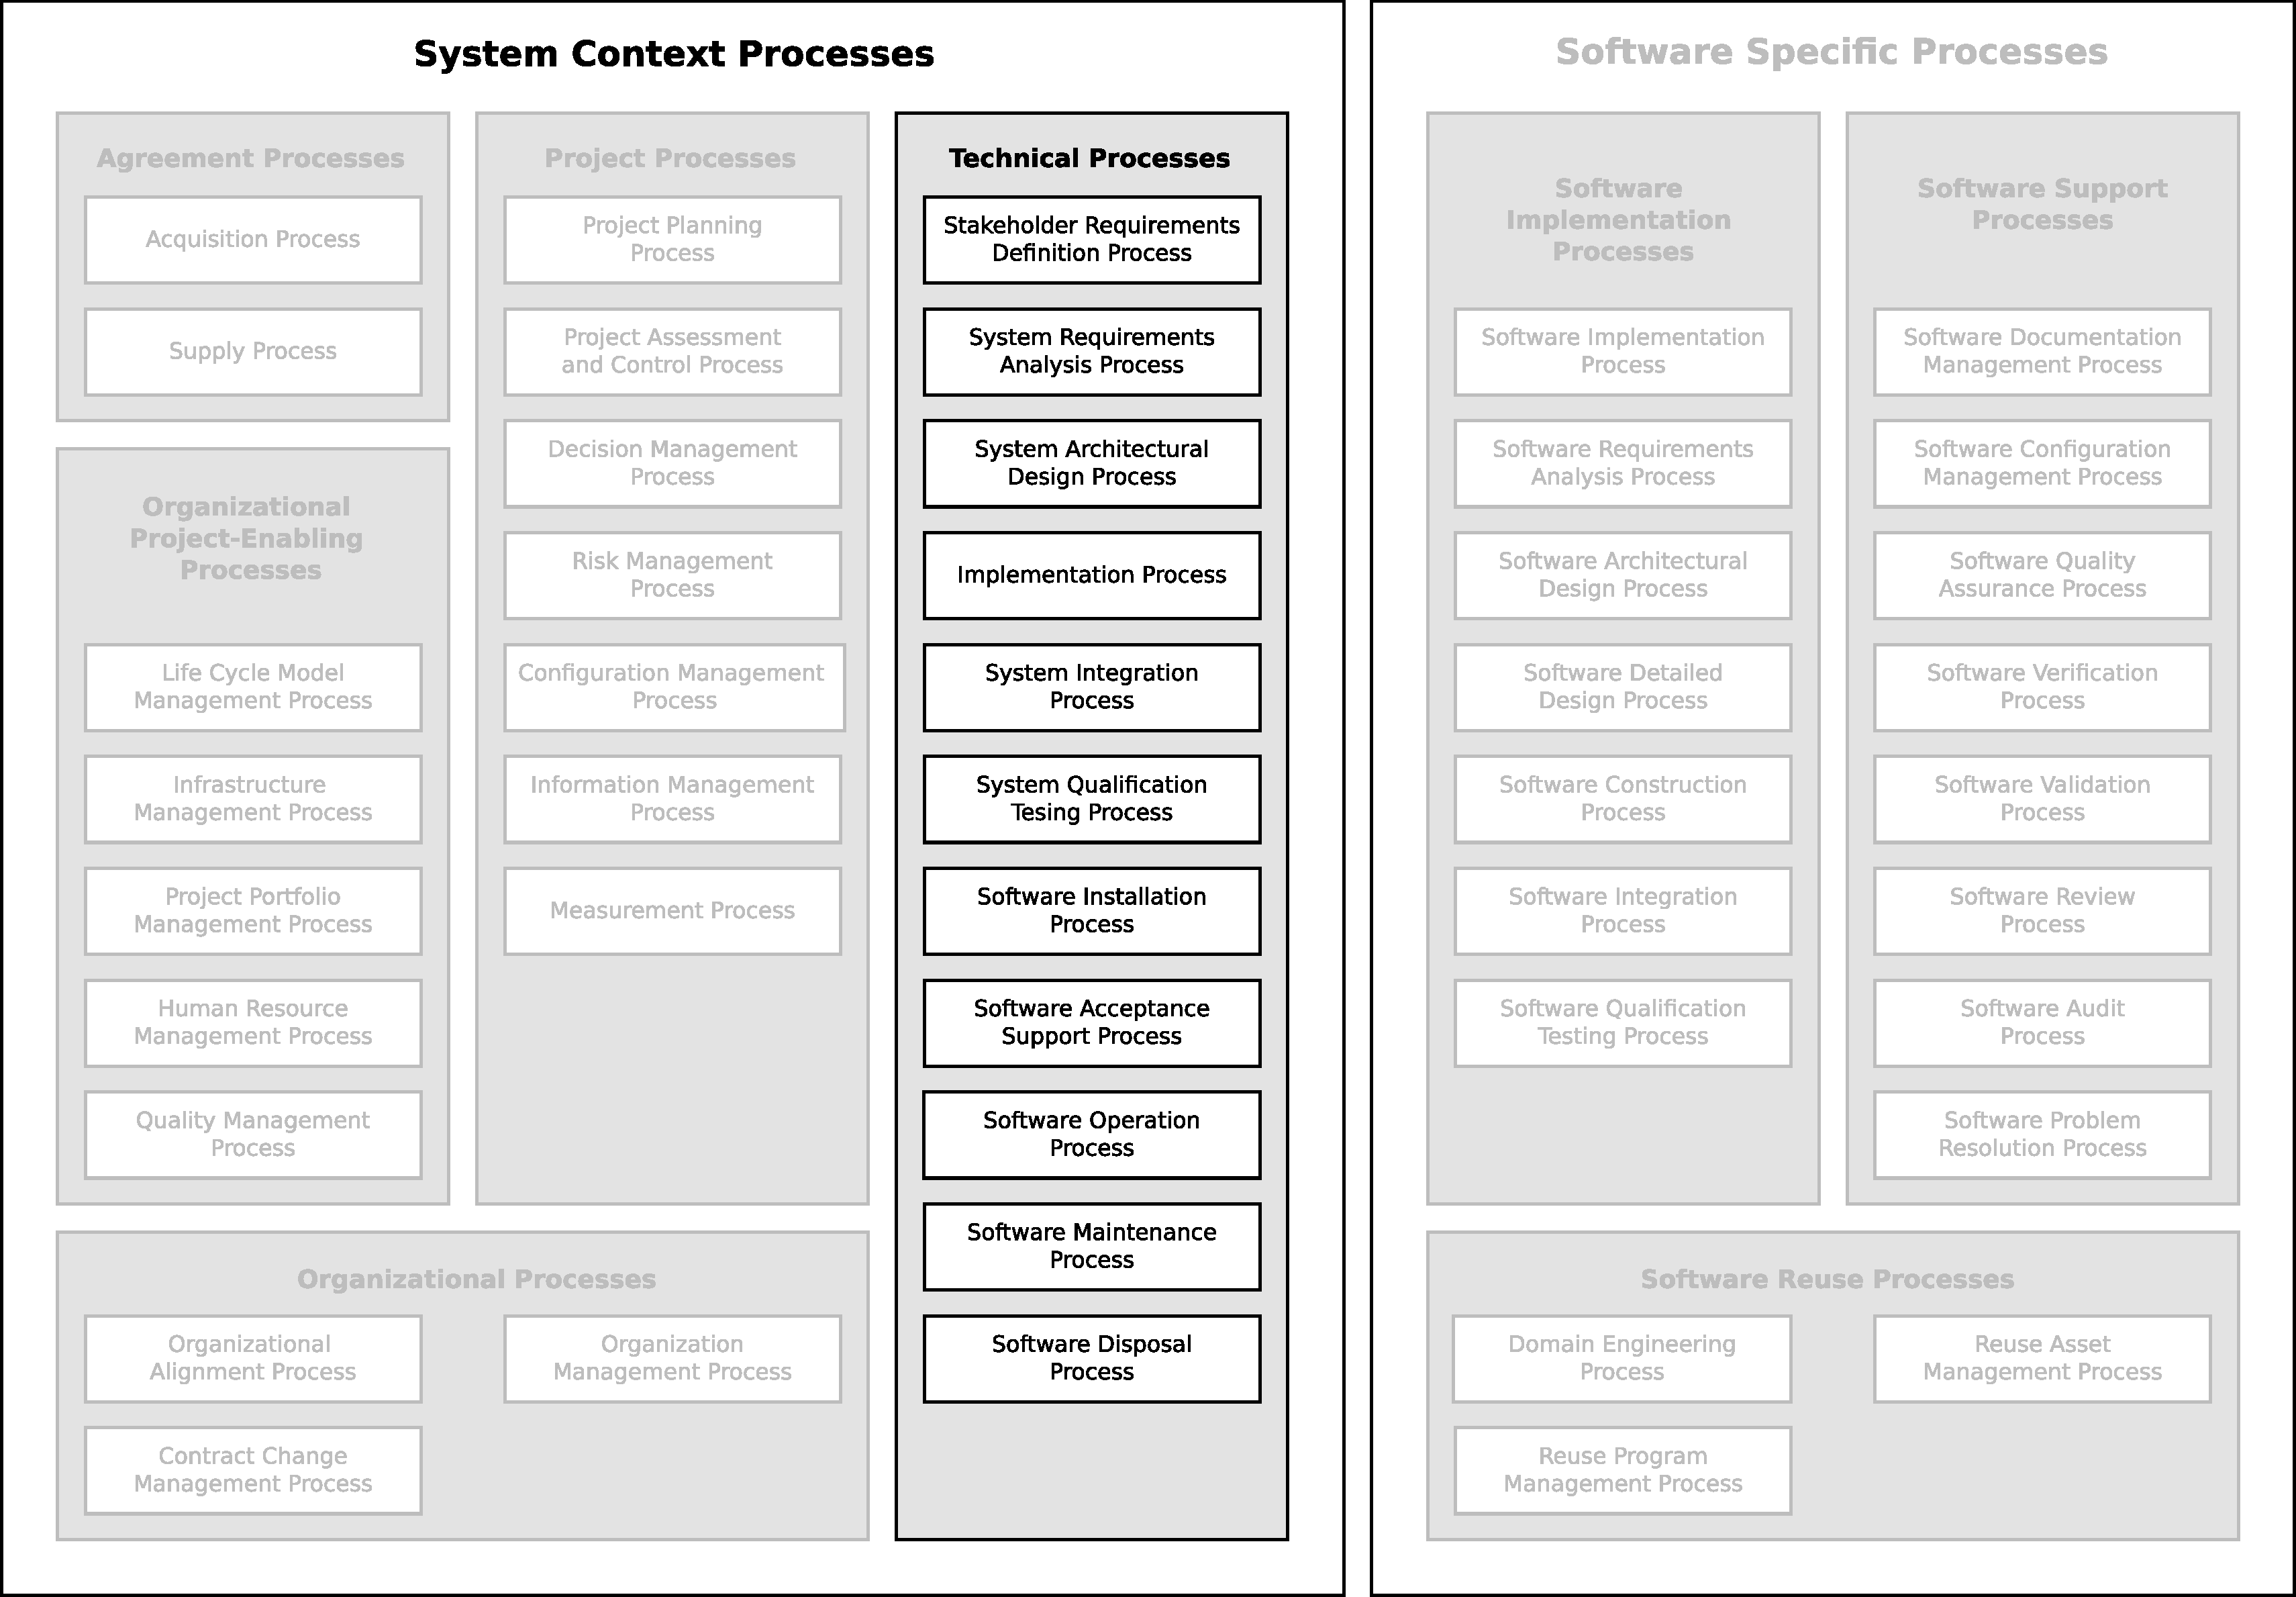
\includegraphics[width=15cm,keepaspectratio]{figures/life-cycle-process-groups-technical-processes.pdf}
			\caption{Technical Processes}
			\label{fig:technical_processes}
		\end{figure}

		\begin{adjustwidth}{1em}{0pt}

			The Technical Processes define the activities that enable organizational and project functions to optimize the benefits and reduce the risks that arise from technical decisions and actions. 

			These activities enable products and services to possess the timeliness and availability, the cost effectiveness, and the functionality, reliability, maintainability, producibility, usability and other qualities required by acquiring and supplying organizations. They also enable products and services to conform to the expectations or legislated requirements of society, including health, safety, security and environmental factors.

			\begin{compactitem}
			
				\item \ref{proc:stakeholder_requirements_definition_process} - \nameref{proc:stakeholder_requirements_definition_process}

				\item \ref{proc:system_requirements_analysis_process} - \nameref{proc:system_requirements_analysis_process}

				\item \ref{proc:system_architectural_design_process} - \nameref{proc:system_architectural_design_process}

				\item \ref{proc:implementation_process} - \nameref{proc:implementation_process}

				\item \ref{proc:system_integration_process} - \nameref{proc:system_integration_process}

				\item \ref{proc:system_qualification_testing_process} - \nameref{proc:system_qualification_testing_process}

				\item \ref{proc:software_installation_process} - \nameref{proc:software_installation_process}

				\item \ref{proc:software_acceptance_support_process} - \nameref{proc:software_acceptance_support_process}

				\item \ref{proc:software_operation_process} - \nameref{proc:software_operation_process}

				\item \ref{proc:software_maintenance_process} - \nameref{proc:software_maintenance_process}

				\item \ref{proc:software_disposal_process} - \nameref{proc:software_disposal_process}
			
			\end{compactitem}

		\end{adjustwidth}

		\newpage
		\subsubsection{STAKEHOLDER REQUIREMENTS DEFINITION PROCESS\label{proc:stakeholder_requirements_definition_process}}

			\subsubsubsection{PURPOSE}
			\begin{adjustwidth}{2em}{0pt} 
			
				The purpose of the \nameref{proc:stakeholder_requirements_definition_process} is to define the requirements for a system that can provide the services needed by users and other stakeholders in a defined environment.

				It identifies stakeholders, or stakeholder classes, involved with the system throughout its life cycle, and their needs and desires. It analyzes and transforms these into a common set of stakeholder requirements that express the intended interaction the system will have with its operational environment and that are the reference against which each resulting operational service is validated in order to confirm that the system fulfills needs.

			\end{adjustwidth}

			\subsubsubsection{OUTCOMES}
			\begin{adjustwidth}{2em}{0pt} 

				\begin{compactitem}

					\item the required characteristics and context of use of services are specified;

					\item the constraints on a system solution are defined;

					\item traceability of stakeholder requirements to stakeholders and their needs is achieved;

					\item the basis for defining the system requirements is described;

					\item the basis for validating the conformance of the services is defined; and

					\item a basis for negotiating and agreeing to supply a service or product is provided.

				\end{compactitem}

			\end{adjustwidth}

			\subsubsubsection{ACTIVITIES AND TASKS}
			\begin{adjustwidth}{2em}{0pt} 

				\begin{compactenum}

					\item {\bf Stakeholder Identification}:
					\begin{compactenum}

						\item The project shall identify the individual stakeholders or stakeholder classes who have a legitimate interest in the system throughout its life cycle.

					\end{compactenum}

					\item {\bf Requirements Identification}:
					\begin{compactenum}

						\item The project shall elicit stakeholder requirements.

						\item The project shall define the constraints on a system solution that are unavoidable consequences of existing agreements, management decisions and technical decisions.

						\item The project shall define a representative set of activity sequences to identify all required services that correspond to anticipated operational and support scenarios and environments.

						\item The project shall identify the interaction between users and the system, taking into the account human capabilities and skills limitations.

						\begin{compactenum}

							\item Physical, mental, and learned capabilities;

							\item Work place, environment and facilities, including other equipment in the context of use;

							\item Normal, unusual, and emergency conditions;

							\item Operator and user recruitment, training and culture.

						\end{compactenum}

						\item The project shall specify health, safety, security, environment and other stakeholder requirements and functions that relate to critical qualities and shall address possible adverse effects of use of the system on human health and safety.

					\end{compactenum}

					\item {\bf Requirements Evaluation}:
					\begin{compactenum}

						\item The project shall analyze the complete set of elicited requirements.

					\end{compactenum}

					\item {\bf Requirements Agreement}:
					\begin{compactenum}

						\item The project shall resolve requirements problems.

						\item The project shall feed back the analyzed requirements to applicable stakeholders to ensure that the needs and expectations have been adequately captured and expressed.

						\item The project shall establish with stakeholders that their requirements are expressed correctly.

					\end{compactenum}

					\item {\bf Requirements Recording}:

					\begin{compactenum}

						\item The project shall record the stakeholder requirements in a form suitable for requirements management through the life cycle and beyond.

						\item The project shall maintain stakeholder requirements traceability to the sources of stakeholder need.

					\end{compactenum}

				\end{compactenum}

			\end{adjustwidth}

		\newpage
		\subsubsection{SYSTEM REQUIREMENTS ANALYSIS PROCESS\label{proc:system_requirements_analysis_process}}

			\subsubsubsection{PURPOSE}
			\begin{adjustwidth}{2em}{0pt} 

				The purpose of \nameref{proc:system_requirements_analysis_process} is to transform the defined stakeholder requirements into a set of desired system technical requirements that will standard the design of the system.

			\end{adjustwidth}

			\subsubsubsection{OUTCOMES}
			\begin{adjustwidth}{2em}{0pt} 

				\begin{compactitem}

					\item a defined set of system functional and non-functional requirements describing the problem to be solved are established;

					\item the appropriate techniques are performed to optimize the preferred project solution;

					\item system requirements are analyzed for correctness and testability;

					\item the impact of the system requirements on the operating environment are understood;

					\item the requirements are prioritized, approved and updated as needed;

					\item consistency and traceability are established between the system requirements and the customer's requirements baseline;

					\item changes to the baseline are evaluated for cost, schedule and technical impact; and

					\item the system requirements are communicated to all affected parties and baselined.

				\end{compactitem}

			\end{adjustwidth}

			\subsubsubsection{ACTIVITIES AND TASKS}
			\begin{adjustwidth}{2em}{0pt} 

				\begin{compactenum}

					\item {\bf Requirements Specification}:

					\begin{compactenum}

						\item The specific intended use of the system to be developed shall be analyzed to specify system requirements. The system requirements specification shall describe: functions and capabilities of the system; business, organizational and user requirements; safety, security, human-factors engineering (ergonomics), interface, operations, and maintenance requirements; design constraints and qualification requirements. The system requirements specification shall be documented.

					\end{compactenum}

					\item {\bf Requirements Evaluation}:

					\begin{compactenum}

						\item The system requirements shall be evaluated considering the criteria listed below. The results of evaluations shall be documented.

						\begin{compactenum}

							\item Traceability to acquisition needs;

							\item Consistency with acquisition needs;

							\item Testability;

							\item Feasibility of system architectural design;

							\item Feasibility of operation and maintenance.

						\end{compactenum}

					\end{compactenum}

				\end{compactenum}

			\end{adjustwidth}

		\newpage
		\subsubsection{SYSTEM ARCHITECTURAL DESIGN PROCESS\label{proc:system_architectural_design_process}}
		
			\subsubsubsection{PURPOSE}
			\begin{adjustwidth}{2em}{0pt} 
				
				The purpose of the \nameref{proc:system_architectural_design_process} is to identify which system requirements should be allocated to which elements of the system.

			\end{adjustwidth}

			\subsubsubsection{OUTCOMES}
			\begin{adjustwidth}{2em}{0pt} 

				\begin{compactitem}

					\item a system architecture design is defined that identifies the elements of the system and meets the defined requirements;

					\item the system's functional and non-functional requirements are addressed;

					\item the requirements are allocated to the elements of the system;

					\item internal and external interfaces of each system element are defined;

					\item verification between the system requirements and the system architecture is performed;

					\item the requirements allocated to the system elements and their interfaces are traceable to the customer's requirements baseline;

					\item consistency and traceability between the system requirements and system architecture design is maintained; and

					\item the system requirements, the system architecture design, and their relationships are baselined and communicated to all affected parties;

					\item human factors and ergonomic knowledge and techniques are incorporated in system design; and

					\item human-centered design activities are identified and performed.

				\end{compactitem}

			\end{adjustwidth}

			\subsubsubsection{ACTIVITIES AND TASKS}
			\begin{adjustwidth}{2em}{0pt} 

				\begin{compactenum}

					\item {\bf Establishing Architecture}:
					\begin{compactenum}

						\item A top-level architecture of the system shall be established. The architecture shall identify items of hardware, software, and manual operations. It shall be ensured that all the system requirements are allocated among the items. Hardware configuration items, software configuration items, and manual operations shall be subsequently identified from these items. The system architecture and the system requirements allocated to the items shall be documented.

					\end{compactenum}

					\item {\bf Architectural Evaluation}:
					\begin{compactenum}

						\item The system architecture and the requirements for the items shall be evaluated considering the criteria listed below. The results of the evaluations shall be documented.

						\begin{compactenum}

							\item Traceability to the system requirements.

							\item Consistency with the system requirements.

							\item Appropriateness of design standards and methods used.

							\item Feasibility of the software items fulfilling their allocated requirements.

							\item Feasibility of operation and maintenance.

						\end{compactenum}

					\end{compactenum}

				\end{compactenum}

			\end{adjustwidth}

		\newpage
		\subsubsection{IMPLEMENTATION PROCESS\label{proc:implementation_process}}

			\subsubsubsection{PURPOSE}
			\begin{adjustwidth}{2em}{0pt} 
				
				The purpose of the \nameref{proc:implementation_process} is to realize a specified system element.

				{\bf Note}: This process is intentionally void of outcomes, activities, and tasks, as the implementation process to realize any given system element is contingent upon the context of that element. See \nameref{proc:software_implementation_process} for how the implementation process is defined for software, as an example. 

			\end{adjustwidth}

		\newpage
		\subsubsection{SYSTEM INTEGRATION PROCESS\label{proc:system_integration_process}}

			\subsubsubsection{PURPOSE}
			\begin{adjustwidth}{2em}{0pt} 

				The purpose of the \nameref{proc:system_integration_process} is to integrate the system elements (including software items, hardware items, manual operations, and other systems, as necessary) to produce a complete system that will satisfy the system design and the customers’ expectations expressed in the system requirements.

			\end{adjustwidth}


			\subsubsubsection{OUTCOMES}
			\begin{adjustwidth}{2em}{0pt} 

				\begin{compactitem}

					\item a strategy is developed to integrate the system according to the priorities of the system requirements;

					\item criteria are developed to verify compliance with the system requirements allocated to the system elements, including the interfaces between system elements;

					\item the system integration is verified using the defined criteria;

					\item a regression strategy is developed and applied for re-testing the system when changes are made;

					\item consistency and traceability are established between the system design and the integrated system elements;

					\item an integrated system is constructed that demonstrates compliance with the system design; and

					\item an integrated system is constructed that demonstrates that a complete set of usable deliverable system elements exists.

				\end{compactitem}

			\end{adjustwidth}

			\subsubsubsection{ACTIVITIES AND TASKS}
			\begin{adjustwidth}{2em}{0pt} 

				\begin{compactenum}

					\item {\bf Integration}:

					\begin{compactenum}

							\item The software configuration items shall be integrated, with hardware configuration items, manual operations, and other systems as necessary, into the system. The aggregates shall be tested, as they are developed, against their requirements. The integration and the test results shall be documented.

					\end{compactenum}

					\item {\bf Test Readiness}:

					\begin{compactenum}

							\item For each qualification requirement of the system, a set of tests, test cases (inputs, outputs, test criteria), and test procedures for conducting System Qualification Testing shall be developed and documented. The developer shall ensure that the integrated system is ready for System Qualification Testing.

							\item The integrated system shall be evaluated considering the criteria listed below. The results of the evaluations shall be documented.

							\begin{compactenum}

								\item Test coverage of system requirements.

								\item Appropriateness of test methods and standards used.

								\item Conformance to expected results.

								\item Feasibility of system qualification testing.

								\item Feasibility of operation and maintenance.

							\end{compactenum}

					\end{compactenum}

				\end{compactenum}

			\end{adjustwidth}

		\newpage
		\subsubsection{SYSTEM QUALIFICATION TESTING PROCESS\label{proc:system_qualification_testing_process}}

			\subsubsubsection{PURPOSE}
			\begin{adjustwidth}{2em}{0pt} 

				The purpose of the \nameref{proc:system_qualification_testing_process} is to ensure that the implementation of each system requirement is tested for compliance and that the system is ready for delivery.

			\end{adjustwidth}

			\subsubsubsection{OUTCOMES}
			\begin{adjustwidth}{2em}{0pt} 

				\begin{compactitem}

					\item criteria for evaluating compliance with system requirements are developed;

					\item the integrated system is tested using the defined criteria;

					\item test results are recorded; and

					\item readiness of the system for delivery is assured.

				\end{compactitem}

			\end{adjustwidth}

			\subsubsubsection{ACTIVITIES AND TASKS}
			\begin{adjustwidth}{2em}{0pt} 

				\begin{compactenum}

					\item {\bf Qualification Testing}:

					\begin{compactenum}

						\item System qualification testing shall be conducted in accordance with the qualification requirements specified for the system. 

						\item It shall be ensured that the implementation of each system requirement is tested for compliance and that the system is ready for delivery.

						\item The qualification testing results shall be documented.

						\item The system shall be evaluated considering the criteria listed below. evaluations shall be documented.

						\begin{compactenum}

							\item Test coverage of system requirements;

							\item Conformance to expected results;

							\item Feasibility of operation and maintenance.

						\end{compactenum}

						\item The developer shall support audit(s) in accordance with \nameref{proc:software_audit_process}. The results of the audit(s) shall be documented.

						\item Upon successful completion of the audit(s), if conducted, the developer shall update and prepare the deliverable software product for Software Installation and Software Acceptance Support.

					\end{compactenum}

				\end{compactenum}

			\end{adjustwidth}

		\newpage
		\subsubsection{SOFTWARE INSTALLATION PROCESS\label{proc:software_installation_process}}

			\subsubsubsection{PURPOSE}
			\begin{adjustwidth}{2em}{0pt} 

				The purpose of the \nameref{proc:software_installation_process} is to install the software product that meets the agreed requirements in the target environment.

			\end{adjustwidth}

			\subsubsubsection{OUTCOMES}
			\begin{adjustwidth}{2em}{0pt} 

				\begin{compactitem}

					\item a software installation strategy is developed;

					\item criteria for software installation are developed that demonstrate compliance with the software installation requirements;

					\item the software product is installed in the target environment; and

					\item readiness of the software product for use in its intended environment is assured.

				\end{compactitem}

			\end{adjustwidth}

			\subsubsubsection{ACTIVITIES AND TASKS}
			\begin{adjustwidth}{2em}{0pt} 

				\begin{compactenum}

					\item {\bf Software Installation}:

					\begin{compactenum}

						\item The implementer shall develop a plan to install the software product in the target environment as designated in the contract. The resources and information necessary to install the software product shall be determined and be available. As specified in the contract, the implementer shall assist the acquirer with the set-up activities.  Where the installed software product is replacing an existing system, the implementer shall support any parallel running activities that are required by contract. The installation plan shall be documented.

						\item The developer shall install the software product in accordance with the installation plan. It shall be ensured that the software code and databases initialize, execute, and terminate as specified in the contract. The installation events and results shall be documented.

					\end{compactenum}

				\end{compactenum}

			\end{adjustwidth}

		\newpage
		\subsubsection{SOFTWARE ACCEPTANCE SUPPORT PROCESS\label{proc:software_acceptance_support_process}}

			\subsubsubsection{PURPOSE}
			\begin{adjustwidth}{2em}{0pt} 

				The purpose of the \nameref{proc:software_acceptance_support_process} is to assist the acquirer to achieve confidence that the product meets requirements.

			\end{adjustwidth}

			\subsubsubsection{OUTCOMES}
			\begin{adjustwidth}{2em}{0pt} 

				\begin{compactitem}

					\item the product is completed and delivered to the acquirer;

					\item acquirer acceptance tests and reviews are supported;

					\item the product is put into operation in the customers’ environment; and

					\item problems detected during acceptance are identified and communicated to those responsible for resolution.

				\end{compactitem}

			\end{adjustwidth}

			\subsubsubsection{ACTIVITIES AND TASKS}
			\begin{adjustwidth}{2em}{0pt} 

				\begin{compactenum}

					\item {\bf Software Acceptance Support}:

					\begin{compactenum}

						\item The developer shall support the acquirer's acceptance review and testing of the software product. Acceptance review and testing shall consider the results of the \nameref{proc:software_review_process}, \nameref{proc:software_audit_process}, \nameref{proc:software_qualification_testing_process}, and \nameref{proc:system_qualification_testing_process} (if performed) processes. The results of the acceptance review and testing shall be documented.

						\item The developer shall complete and deliver the software product as specified in the contract.

						\item The developer shall provide initial and continuing training and support to the acquirer as specified in the contract.

					\end{compactenum}

				\end{compactenum}

			\end{adjustwidth}

		\newpage
		\subsubsection{SOFTWARE OPERATION PROCESS\label{proc:software_operation_process}}

			\subsubsubsection{PURPOSE}
			\begin{adjustwidth}{2em}{0pt} 
				
				The purpose of the \nameref{proc:software_operation_process} is to operate the software product in its intended environment and to provide support to the customers of the software product.

			\end{adjustwidth}

			\subsubsubsection{OUTCOMES}
			\begin{adjustwidth}{2em}{0pt} 

				\begin{compactitem}

					\item an operation strategy is defined;

					\item conditions for correct operation of the software in its intended environment are identified and evaluated;

					\item the software is tested and determined to operate in its intended environment;

					\item the software is operated in its intended environment; and

					\item assistance and consultation is provided to the customers of the software product in accordance with the agreement.

				\end{compactitem}

			\end{adjustwidth}

			\subsubsubsection{ACTIVITIES AND TASKS}
			\begin{adjustwidth}{2em}{0pt} 

				\begin{compactenum}

					\item {\bf Preparation for Operation}:

					\begin{compactenum}

						\item The operator shall develop a plan and set operational standards for performing the activities and tasks of this process. The plan shall be documented and executed.

						\item The operator shall establish procedures for receiving, recording, resolving, tracking problems, and providing feedback. Whenever problems are encountered, they shall be recorded and entered into the \nameref{proc:software_problem_resolution_process}.

						\item The operator shall establish procedures for testing the software product in its operation environment, for entering problem reports and modification requests to the \nameref{proc:software_maintenance_process}, and for releasing the software product for operational use.

					\end{compactenum}

					\item {\bf Operation Activation and Check-out}:

					\begin{compactenum}

						\item For each release of the software product, the operator shall perform operational testing, and, on satisfying the specified criteria, release the software product for operational use.

						\item The operator shall ensure that the software code and databases initialize, execute, and terminate as described in the plan.

						\item The operator shall activate the system in its intended operational situation to deliver instances of service or continuous service according to its intended purpose.

					\end{compactenum}

					\item {\bf Operational Use}:

					\begin{compactenum}

						\item The system shall be operated in its intended environment according to the user documentation.

					\end{compactenum}

					\item {\bf Customer Support}:

					\begin{compactenum}

						\item The operator shall provide assistance and consultation to the users as requested. These requests and subsequent actions shall be recorded and monitored.

						\item The operator shall forward user requests, as necessary, to the \nameref{proc:software_maintenance_process} for resolution. These requests shall be addressed and the actions that are planned and taken shall be reported to the originators of the requests. All resolutions shall be monitored to conclusion.

					\end{compactenum}

					\item {\bf Operational Problem Resolution}:

					\begin{compactenum}

						\item The operator shall forward identified problems to the Software Problem Resolution Process for resolution.

						\item If a reported problem has a temporary work-around before a permanent solution can be released, the originator of the problem report shall be given the option to use it. Permanent corrections, releases that include previously omitted functions or features, and system improvements shall be applied to the operational software product using the \nameref{proc:software_maintenance_process}.

					\end{compactenum}

				\end{compactenum}

			\end{adjustwidth}

		\newpage
		\subsubsection{SOFTWARE MAINTENANCE PROCESS\label{proc:software_maintenance_process}}

			\subsubsubsection{PURPOSE}
			\begin{adjustwidth}{2em}{0pt}  

				The purpose of the \nameref{proc:software_maintenance_process} is to provide cost-effective support to a delivered software product.

				{\bf Note}: Pre-delivery Software Maintenance activities include planning for post-delivery operations, supportability, and logistics determination. Post-delivery activities include software modification and operational support, such as training or operating a help desk.

			\end{adjustwidth}

			\subsubsubsection{OUTCOMES}
			\begin{adjustwidth}{2em}{0pt} 

				\begin{compactitem}

					\item a maintenance strategy is developed to manage modification and migration of products according to the release strategy;

					\item the impact of changes to the existing system on organization, operations or interfaces are identified;

					\item affected system and software documentation is updated as needed;

					\item modified products are developed with associated tests that demonstrate that requirements are not compromised;

					\item product upgrades are migrated to the customer’s environment; and

					\item the system software modification is communicated to all affected parties.

				\end{compactitem}

			\end{adjustwidth}

			\subsubsubsection{ACTIVITIES AND TASKS}
			\begin{adjustwidth}{2em}{0pt} 

				\begin{compactenum}

					\item {\bf Process Implementation}:

					\begin{compactenum}

						\item The maintainer shall develop, document, and execute plans and procedures for conducting the activities and tasks of the Software Maintenance Process.

						\item The maintainer shall establish procedures for receiving, recording, and tracking problem reports and modification requests from the users and providing feedback to the users. Whenever problems are encountered, they shall be recorded and entered into the \nameref{proc:software_problem_resolution_process}.

						\item The maintainer shall implement (or establish organizational interface with) the \nameref{proc:configuration_management_process} for managing modifications to the existing system.

					\end{compactenum}


					\item {\bf Problem and Modification Analysis}:

					\begin{compactenum}

						\item The maintainer shall analyze the problem report or modification request for its impact on the organization, the existing system, and the interfacing systems for the following:

						\begin{compactenum}

							\item Type; for example, corrective, improvement, preventive, or adaptive to new environment;

							\item Scope; for example, size of modification, cost involved, time to modify;

							\item Criticality; for example, impact on performance, safety, or security.

						\end{compactenum}

						\item The maintainer shall replicate or verify the problem.

						\item The maintainer shall document the problem/modification request, the analysis results, and implementation options.

						\item The maintainer shall obtain approval for the selected modification option as specified in the contract. 

					\end{compactenum}


					\item {\bf Modification Implementation}:

					\begin{compactenum}

						\item The maintainer shall conduct analysis and determine which documentation, software units, and versions thereof need to be modified. These shall be documented.

						\item The maintainer shall enter the \nameref{subsec:technical_processes} to implement the modifications. The requirements of the Technical Processes shall be supplemented as follows:

						\item Test and evaluation criteria for testing and evaluating the modified and the unmodified parts (software units, components, and configuration items) of the system shall be defined and documented.

						\item The complete and correct implementation of the new and modified requirements shall be ensured. It also shall be ensured that the original, unmodified requirements were not affected. The test results shall be documented.

					\end{compactenum}

					\item {\bf Maintenance Review/Acceptance}:

					\begin{compactenum}

						\item The maintainer shall conduct review(s) with the organization authorizing the modification to determine the integrity of the modified system.

						\item The maintainer shall obtain approval for the satisfactory completion of the modification as specified in the contract.

					\end{compactenum}

					\item {\bf Migration}:

					\begin{compactenum}

						\item If a system or software product (including data) is migrated from an old to a new operational environment, it shall be ensured that any software product or data produced or modified during migration is in accordance with this standard.

						\item A migration plan shall be developed, documented, and executed. The planning activities shall include users. Items included in the plan shall include the following:

						\begin{compactenum}

							\item Requirements analysis and definition of migration.

							\item Development of migration tools.

							\item Conversion of software product and data.

							\item Migration execution.

							\item Migration verification.

							\item Support for the old environment in the future.

						\end{compactenum}

						\item Users shall be given notification of the migration plans and activities. Notifications shall include the following:

						\begin{compactenum}

							\item Statement of why the old environment is no longer to be supported.

							\item Description of the new environment with its date of availability.

							\item Description of other support options available, if any, once support for the old environment has been removed.

						\end{compactenum}


						\item Parallel operations of the old and new environments may be conducted for smooth transition to the new environment. During this period, necessary training shall be provided as specified in the contract.

						\item When the scheduled migration arrives, notification shall be sent to all concerned. Associated old environment documentation, logs, and code should be placed in archives.

						\item A post-operation review shall be performed to assess the impact of changing to the new environment. The results of the review shall be sent to the appropriate authorities for information, guidance, and action.

						\item Data used by or associated with the old environment shall be accessible in accordance with the contract requirements for data protection and audit applicable to the data.

					\end{compactenum}

				\end{compactenum}

			\end{adjustwidth}

		\newpage
		\subsubsection{SOFTWARE DISPOSAL PROCESS\label{proc:software_disposal_process}}

			\subsubsubsection{PURPOSE}
			\begin{adjustwidth}{2em}{0pt} 

				The purpose of the \nameref{proc:software_disposal_process} is to end the existence of a system's software entity. This process ends active support by the operation and maintenance organization, or deactivates, disassembles and removes the affected software products, consigning them to a final condition and leaving the environment in an acceptable condition. 

				This process destroys or stores system software elements and related products in a sound manner, in accordance with legislation, agreements, organizational constraints and stakeholder requirements. Where required, it maintains records that may be monitored.
				
				{\bf Note}: The objective is to retire a system's existing software products or services while preserving the integrity of organizational operations.
			
			\end{adjustwidth}

			\subsubsubsection{OUTCOMES}
			\begin{adjustwidth}{2em}{0pt} 

				\begin{compactitem}

					\item a software disposal strategy is defined;

					\item disposal constraints are provided as inputs to requirements;

					\item the system's software elements are destroyed or stored;

					\item the environment is left in an agreed-upon state; and

					\item records allowing knowledge retention of disposal actions and any analysis of long-term impacts are available.

				\end{compactitem}

			\end{adjustwidth}

			\subsubsubsection{ACTIVITIES AND TASKS}
			\begin{adjustwidth}{2em}{0pt} 

				\begin{compactenum}

					\item {\bf Software Disposal Planning}:

					\begin{compactenum}

						\item A software disposal strategy is defined and documented. A plan to remove active support by the operation and maintenance organizations shall be developed and documented. The planning activities shall include users. The software disposal plan shall address the items listed below:

						\begin{compactenum}

							\item Cessation of full or partial support after a certain period of time.

							\item Archiving of the software product and its associated documentation.

							\item Responsibility for any future residual support issues.

							\item Transition to any new software product, if applicable.

							\item Accessibility of archive copies of data.

						\end{compactenum}

					\end{compactenum}

					\item {\bf Software Disposal Execution}:

					\begin{compactenum}

						\item The software disposal plan shall be executed.

						\item Users shall be given notification of the plans and activities for the retirement of software products and services. Notifications shall include the following:

						\begin{compactenum}

							\item Description of any replacement or upgrade with its date of availability.

							\item Statement of why the software product is no longer to be supported.

							\item Description of other support options available, once support has been removed.

						\end{compactenum}

						\item Parallel operations of the retiring and any new software product should be conducted for smooth transition to the new system. During this period, user training shall be provided as specified in the contract.

						\item When the scheduled retirement arrives, notification shall be sent to all concerned. All associated development documentation, logs, and code should be placed in archives, when appropriate.

						\item Data used by, or associated with, the retired software product shall be accessible in accordance with the contract requirements for data protection and audit applicable to the data.

					\end{compactenum}

				\end{compactenum}

			\end{adjustwidth}

	\newpage
	\section{SOFTWARE SPECIFIC PROCESSES \label{sec:software_specific_processes}}

	\subsection{SOFTWARE IMPLEMENTATION PROCESSES\label{subsec:software_implementation_processes}}

		\begin{figure}[h]
			\centering
			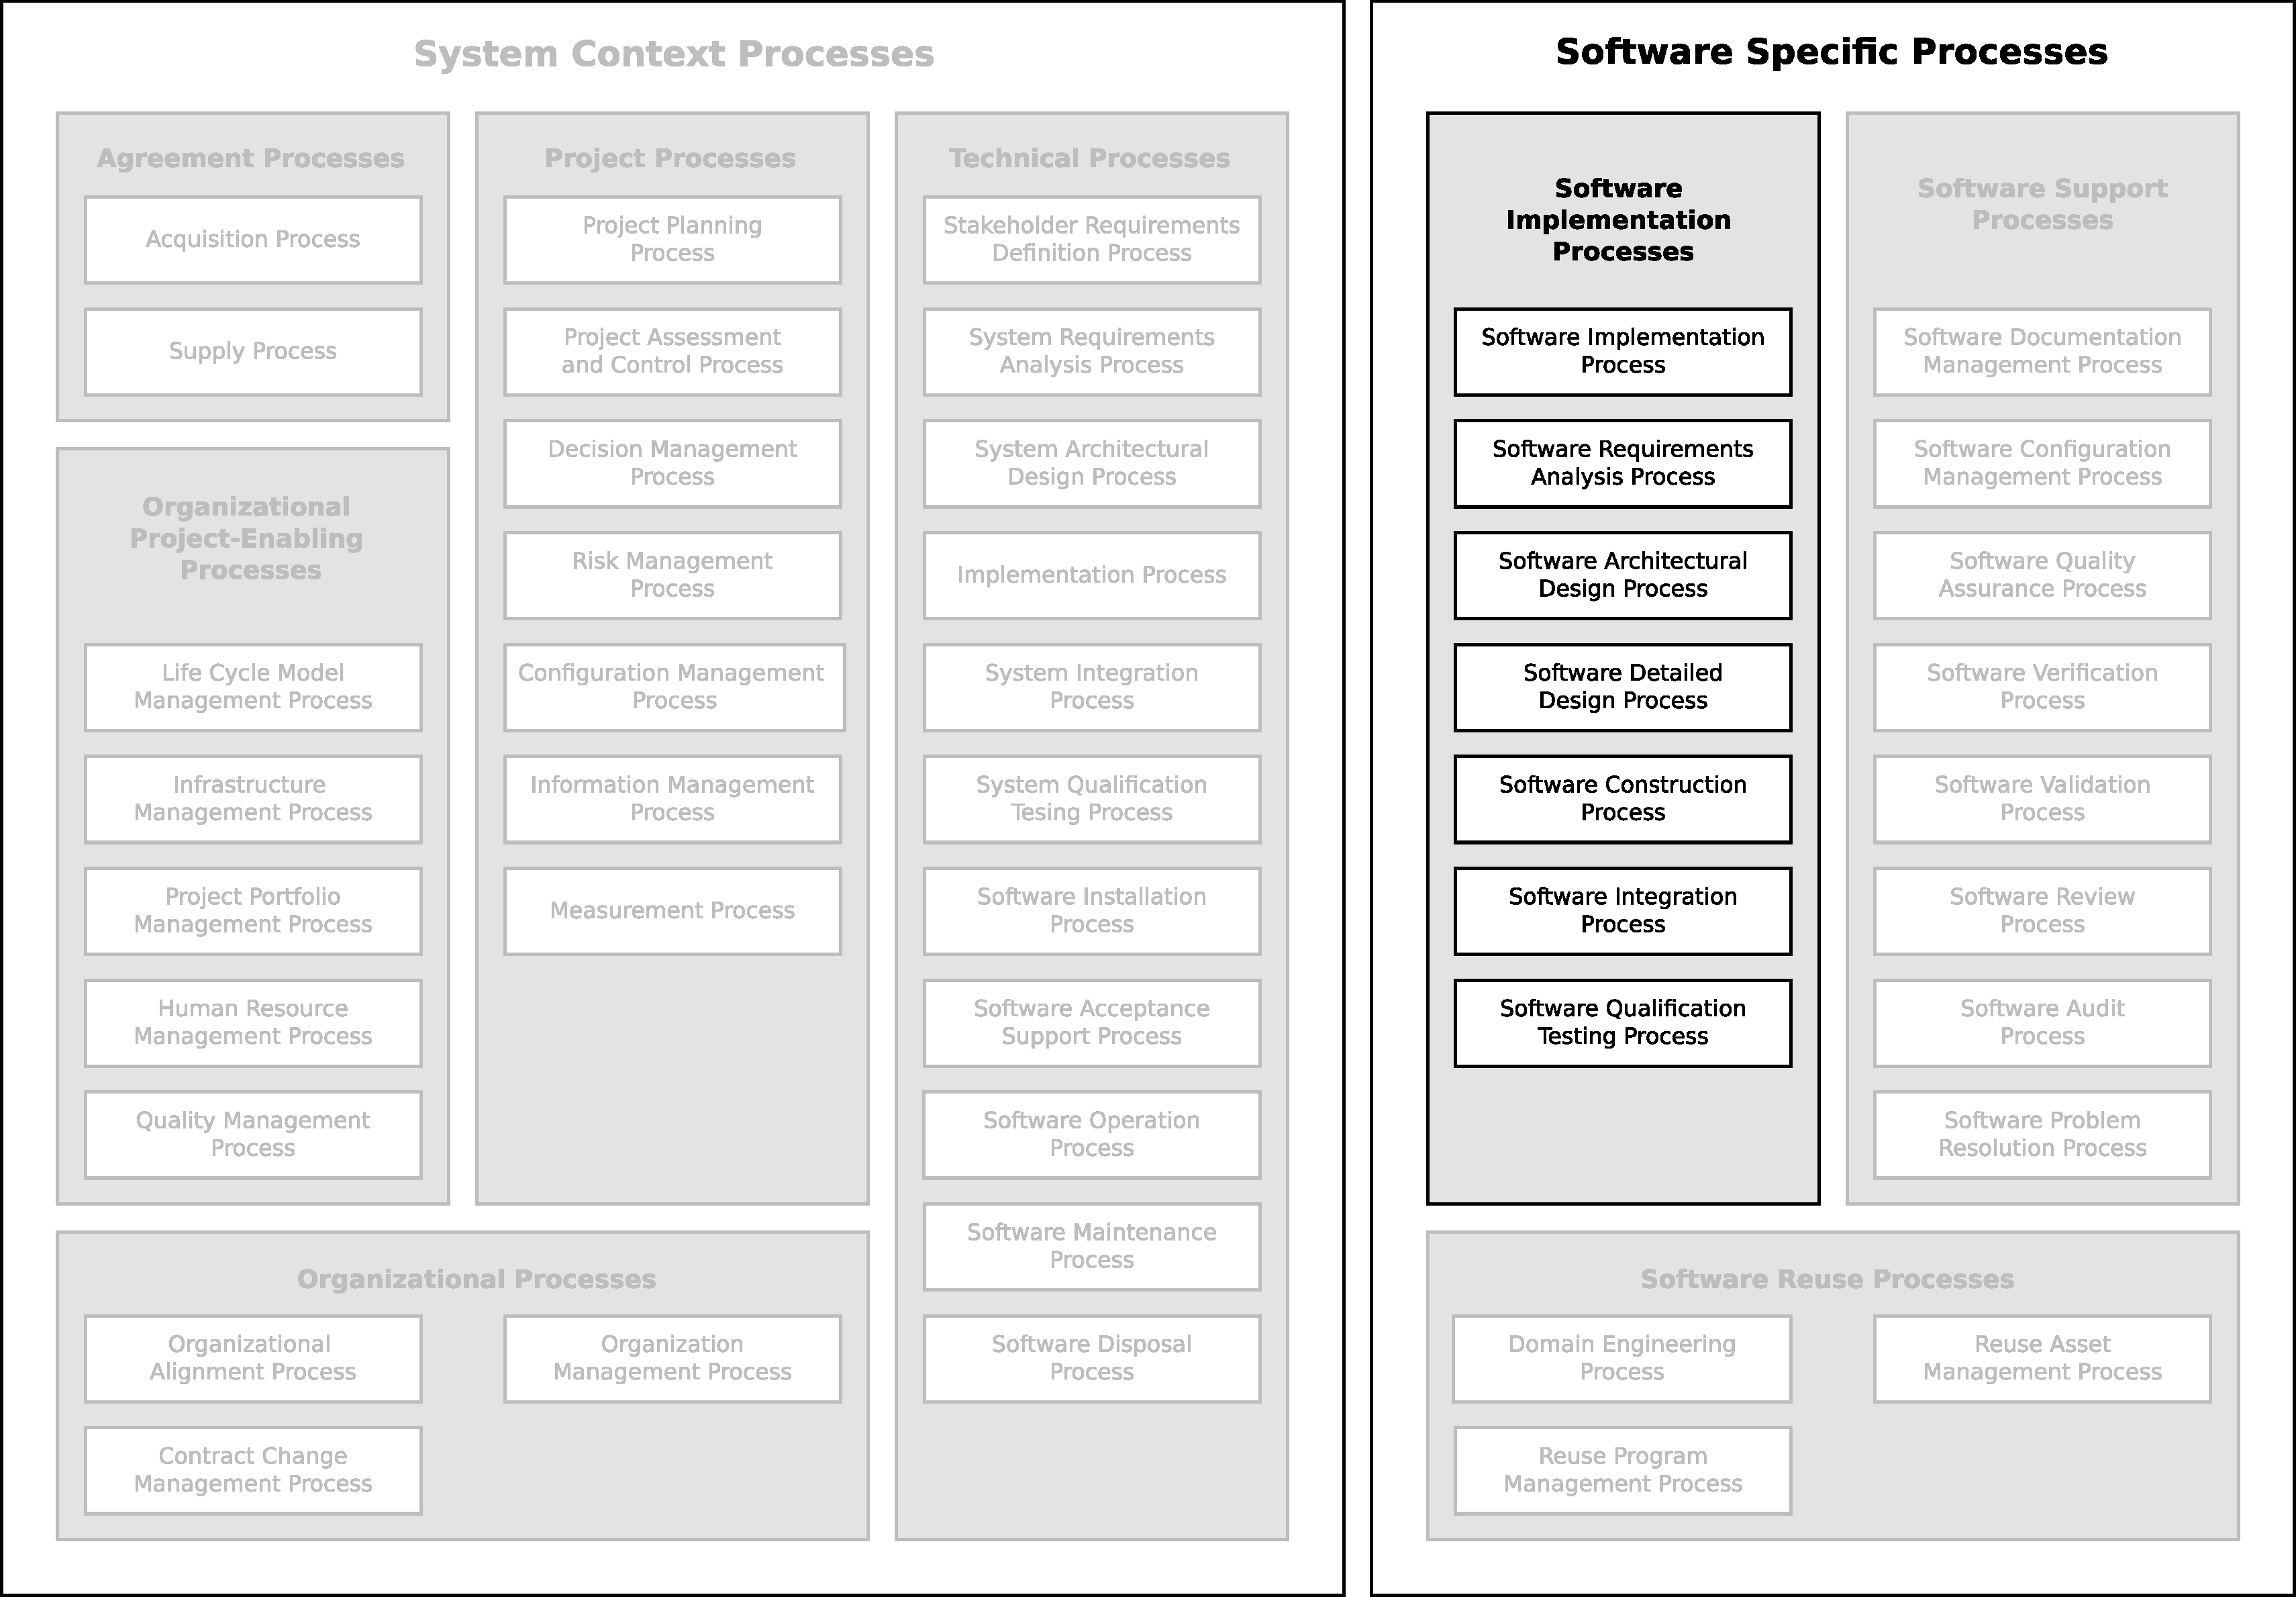
\includegraphics[width=15cm,keepaspectratio]{figures/life-cycle-process-groups-software-implementation-processes.pdf}
			\caption{Software Implementation Processes}
			\label{fig:software_implementation_processes}
		\end{figure}

		\begin{adjustwidth}{1em}{0pt}

			The \nameref{subsec:software_implementation_processes} are used to produce a specified system element (software item) implemented in software. Those processes transform specified behavior, interfaces and implementation constraints into implementation actions resulting in a system element that satisfies the requirements derived from the system requirements.

			\begin{compactitem}
				
				\item \ref{proc:software_implementation_process} - \nameref{proc:software_implementation_process}

				\item \ref{proc:software_requirements_analysis_process} - \nameref{proc:software_requirements_analysis_process}

				\item \ref{proc:software_architectural_design_process} - \nameref{proc:software_architectural_design_process}

				\item \ref{proc:software_detailed_design_process} - \nameref{proc:software_detailed_design_process}

				\item \ref{proc:software_construction_process} - \nameref{proc:software_detailed_design_process}

				\item \ref{proc:software_construction_process} - \nameref{proc:software_construction_process}

				\item \ref{proc:software_integration_process} - \nameref{proc:software_integration_process}

				\item \ref{proc:software_qualification_testing_process} - \nameref{proc:software_qualification_testing_process}

			\end{compactitem}

		\end{adjustwidth}

		\newpage
		\subsubsection{SOFTWARE IMPLEMENTATION PROCESS\label{proc:software_implementation_process}}

			\subsubsubsection{PURPOSE}
			\begin{adjustwidth}{2em}{0pt} 

				The purpose of the \nameref{proc:software_implementation_process} is to produce a specified system element implemented as a software product or service.

				This process transforms specified behavior, interfaces and implementation constraints into actions that create a system element implemented as a software product or service, otherwise known as a ``software item''. 

				This process results in a software item that satisfies architectural design requirements through verification and stakeholder requirements through validation.

			\end{adjustwidth}

			\subsubsubsection{OUTCOMES}
			\begin{adjustwidth}{2em}{0pt} 

				\begin{compactitem}

					\item an implementation strategy is defined;

					\item implementation technology constraints on the design are identified;

					\item a software item is realized; and

					\item a software item is packaged and stored in accordance with an agreement for its supply.

					\item In addition to its activities, this process has the following lower-level processes:

					\begin{compactenum}

						\item Software Architectural Design Process

						\item Software Detailed Design Process

						\item Software Construction Process

						\item Software Integration Process

						\item Software Qualification Testing Process

					\end{compactenum}

				\end{compactitem}

			\end{adjustwidth}

			\subsubsubsection{ACTIVITIES AND TASKS}
			\begin{adjustwidth}{2em}{0pt} 

				\begin{compactenum}

					\item {\bf Software Implementation Strategy}:

					\begin{compactenum}

						\item If not stipulated in the contract, the developer shall define or select a life cycle model appropriate to the scope, magnitude, and complexity of the project. The life cycle model shall be comprised of stages and the purpose and outcomes of each stage. The activities and tasks of the Software Implementation Process shall be selected and mapped onto the life cycle model.

						\item The implementer shall:

						\begin{compactenum}

							\item Document the outputs in accordance with the \nameref{proc:software_documentation_management_process}.

							\item Place the outputs under the \nameref{proc:software_configuration_management_process} and perform change control in accordance with it.

							\item Document and resolve problems and non-conformances found in the software products and tasks in accordance with the \nameref{proc:software_problem_resolution_process}.

							\item Perform supporting processes as specified in the contract.

							\item Establish baselines and incorporate configuration items at appropriate times, as determined by the acquirer and the supplier.

						\end{compactenum}

						\item The implementer shall select, tailor, and use those standards, methods, tools, and computer programming languages (if not stipulated in the contract) that are documented, appropriate, and established by the organization for performing the activities of the Software Implementation Process and supporting processes.

						\item The implementer shall develop plans for conducting the activities of the Software Implementation process. The plans should include specific standards, methods, tools, actions, and responsibility associated with the development and qualification of all requirements including safety and security. If necessary, separate plans may be developed. These plans shall be documented and executed.

						\item Non-deliverable items may be employed in the development or maintenance of the software product. However, it shall be ensured that the operation and maintenance of the deliverable software product after its delivery to the acquirer are independent of such items; otherwise, those items should be considered as deliverable.

					\end{compactenum}

				\end{compactenum}

			\end{adjustwidth}

		\newpage
		\subsubsection{SOFTWARE REQUIREMENTS ANALYSIS PROCESS\label{proc:software_requirements_analysis_process}}

			\subsubsubsection{PURPOSE}
			\begin{adjustwidth}{2em}{0pt} 

				The purpose of \nameref{proc:software_requirements_analysis_process} is to establish the requirements of the software elements of the system.

			\end{adjustwidth}

			\subsubsubsection{OUTCOMES}
			\begin{adjustwidth}{2em}{0pt} 

				\begin{compactitem}

					\item the requirements allocated to the software elements of the system and their interfaces are defined;

					\item software requirements are analyzed for correctness and testability;

					\item the impact of software requirements on the operating environment are understood;

					\item consistency and traceability are established between the software requirements and system requirements;

					\item prioritization for implementing the software requirements is defined;

					\item the software requirements are approved and updated as needed;

					\item changes to the software requirements are evaluated for cost, schedule and technical impact; and

					\item the software requirements are baselined and communicated to all affected parties.

				\end{compactitem}

			\end{adjustwidth}

			\subsubsubsection{ACTIVITIES AND TASKS}
			\begin{adjustwidth}{2em}{0pt} 

				\begin{compactenum}

					\item {\bf Software Requirements Analysis}:

					\begin{compactenum}

						\item The implementer shall establish and document software requirements (including the quality characteristics specifications) described below.

						\begin{compactenum}

							\item Functional and capability specifications, including performance, physical characteristics, environmental conditions under which the software item is to perform.

							\item Interfaces external to the software item.

							\item Qualification requirements.

							\item Safety specifications, including those related to methods of operation and maintenance, environmental influences, and personnel injury.

							\item Security specifications, including those related to compromise of sensitive information.

							\item Human-factors engineering (ergonomics) specifications, including those related to manual operations, human-equipment interactions, constraints on personnel, and areas needing concentrated human attention, that are sensitive to human errors and training.

							\item Data definition and database requirements.

							\item Installation and acceptance requirements of the delivered software product at the operation and maintenance site(s).

							\item User documentation requirements.

							\item User operation and execution requirements.

							\item User maintenance requirements.

						\end{compactenum}

						\item The implementer shall evaluate the software requirements considering the criteria listed below. The results of the evaluations shall be documented.

						\begin{compactenum}

							\item Traceability to system requirements and system design.

							\item External consistency with system requirements.

							\item Internal consistency.

							\item Testability.

							\item Feasibility of software design.

							\item Feasibility of operation and maintenance.

						\end{compactenum}

						\item The implementer shall conduct review(s) in accordance with \nameref{proc:software_review_process}.

					\end{compactenum}

				\end{compactenum}

			\end{adjustwidth}

		\newpage
		\subsubsection{SOFTWARE ARCHITECTURAL DESIGN PROCESS\label{proc:software_architectural_design_process}}

			\subsubsubsection{PURPOSE}
			\begin{adjustwidth}{2em}{0pt} 
				
				The purpose of the \nameref{proc:software_architectural_design_process} is to provide a design for the software that implements and can be verified against the requirements.

			\end{adjustwidth}

			\subsubsubsection{OUTCOMES}
			\begin{adjustwidth}{2em}{0pt} 

				\begin{compactitem}

					\item a software architectural design is developed and baselined that describes the software items that will implement the software requirements;

					\item internal and external interfaces of each software item are defined; and

					\item consistency and traceability are established between software requirements and software design.

				\end{compactitem}

			\end{adjustwidth}

			\subsubsubsection{ACTIVITIES AND TASKS}
			\begin{adjustwidth}{2em}{0pt} 

				\begin{compactenum}

					\item {\bf Software Architectural Design}:

					\begin{compactenum}

						\item The implementer shall transform the requirements for the software item into an architecture that describes its top-level structure and identifies the software components. It shall be ensured that all the requirements for the software item are allocated to its software components and further refined to facilitate detailed design. The architecture of the software item shall be documented.

						\item The implementer shall develop and document a top-level design for the interfaces external to the software item and between the software components of the software item.

						\item The implementer shall develop and document a top-level design for the database.

						\item The implementer should develop and document preliminary versions of user documentation.

						\item The implementer shall define and document preliminary test requirements and the schedule for Software Integration.

						\item The implementer shall evaluate the architecture of the software item and the interface and database designs considering the criteria listed below. The results of the evaluations shall be documented.

						\begin{compactenum}

							\item Traceability to the requirements of the software item.

							\item External consistency with the requirements of the software item.

							\item Internal consistency between the software components.

							\item Appropriateness of design methods and standards used.

							\item Feasibility of detailed design.

							\item Feasibility of operation and maintenance.

						\end{compactenum}

						\item The implementer shall conduct review(s) in accordance with \nameref{proc:software_review_process}

					\end{compactenum}

				\end{compactenum}

			\end{adjustwidth}

		\newpage
		\subsubsection{SOFTWARE DETAILED DESIGN PROCESS\label{proc:software_detailed_design_process}}

			\subsubsubsection{PURPOSE}
			\begin{adjustwidth}{2em}{0pt} 

				The purpose of the \nameref{proc:software_detailed_design_process} is to provide a design for the software that implements and can be verified against the requirements and the software architecture and is sufficiently detailed to permit coding and testing.

			\end{adjustwidth}

			\subsubsubsection{OUTCOMES}
			\begin{adjustwidth}{2em}{0pt} 

				\begin{compactitem}

					\item a detailed design of each software component, describing the software units to be built, is developed;

					\item external interfaces of each software unit are defined; and

					\item consistency and traceability are established between the detailed design and the requirements and architectural design.

				\end{compactitem}

			\end{adjustwidth}

			\subsubsubsection{ACTIVITIES AND TASKS}
			\begin{adjustwidth}{2em}{0pt} 

				\begin{compactenum}

					\item {\bf Software Detailed Design}:

					\begin{compactenum}

						\item The implementer shall develop a detailed design for each software component of the software item. The software components shall be refined into lower levels containing software units that can be coded, compiled, and tested. It shall be ensured that all the software requirements are allocated from the software components to software units. The detailed design shall be documented.

						\item The implementer shall develop and document a detailed design for the interfaces external to the software item, between the software components, and between the software units. The detailed design of the interfaces shall permit coding without the need for further information.

						\item The implementer shall develop and document a detailed design for the database.

						\item The implementer shall update user documentation as necessary.

						\item The implementer shall define and document test requirements and the schedule for testing software units. The test requirements should include stressing the software unit at the limits of its requirements.

						\item The implementer shall update the test requirements and the schedule for Software Integration.

						\item The implementer shall evaluate the software detailed design and test requirements considering the criteria listed below. The results of the evaluations shall be documented.

						\begin{compactenum}

							\item Traceability to the requirements of the software item;

							\item External consistency with architectural design;

							\item Internal consistency between software components and software units;

							\item Appropriateness of design methods and standards used;

							\item Feasibility of testing;

							\item Feasibility of operation and maintenance.

						\end{compactenum}

						\item The implementer shall conduct review(s) in accordance with the \nameref{proc:software_review_process}.

					\end{compactenum}

				\end{compactenum}

			\end{adjustwidth}

		\newpage
		\subsubsection{SOFTWARE CONSTRUCTION PROCESS\label{proc:software_construction_process}}

			\subsubsubsection{PURPOSE}
			\begin{adjustwidth}{2em}{0pt} 
				
				The purpose of the \nameref{proc:software_construction_process} is to produce executable software units that properly reflect the software design.

			\end{adjustwidth}

			\subsubsubsection{OUTCOMES}
			\begin{adjustwidth}{2em}{0pt} 

				\begin{compactitem}

					\item verification criteria are defined for all software units against their requirements;

					\item software units defined by the design are produced;

					\item consistency and traceability are established between software units and requirements and design; and

					\item verification of the software units against the requirements and the design is accomplished.

				\end{compactitem}

			\end{adjustwidth}

			\subsubsubsection{ACTIVITIES AND TASKS}
			\begin{adjustwidth}{2em}{0pt} 

				\begin{compactenum}

					\item {\bf Software Construction}:

					\begin{compactenum}

						\item The implementer shall develop and document the following:

						\item Each software unit and database.

						\item Test procedures and data for testing each software unit and database.

						\item The implementer shall test each software unit and database ensuring that it satisfies its requirements. The test results shall be documented.

						\item The implementer shall update the user documentation as necessary.

						\item The implementer shall update the test requirements and the schedule for Software Integration.

						\item The implementer shall evaluate software code and test results considering the criteria listed below. The results of the evaluations shall be documented.

						\begin{compactenum}

							\item Traceability to the requirements and design of the software item.

							\item External consistency with the requirements and design of the software item.

							\item Internal consistency between unit requirements.

							\item Test coverage of units.

							\item Appropriateness of coding methods and standards used.

							\item Feasibility of software integration and testing.

							\item Feasibility of operation and maintenance.

						\end{compactenum}

					\end{compactenum}

				\end{compactenum}

			\end{adjustwidth}

		\newpage
		\subsubsection{SOFTWARE INTEGRATION PROCESS\label{proc:software_integration_process}}

			\subsubsubsection{PURPOSE}
			\begin{adjustwidth}{2em}{0pt} 

				The purpose of the \nameref{proc:software_integration_process} is to combine the software units and software components, producing integrated software items, consistent with the software design, that demonstrate that the functional and non-functional software requirements are satisfied on an equivalent or complete operational platform.

			\end{adjustwidth}

			\subsubsubsection{OUTCOMES}
			\begin{adjustwidth}{2em}{0pt} 

				\begin{compactitem}

					\item an integration strategy is developed for software units consistent with the software design and the prioritized software requirements;

					\item verification criteria for software items are developed that ensure compliance with the software requirements allocated to the items;

					\item software items are verified using the defined criteria;

					\item software items defined by the integration strategy are produced;

					\item results of integration testing are recorded;

					\item consistency and traceability are established between software design and software items; and

					\item a regression strategy is developed and applied for re-verifying software items when a change in software units (including associated requirements, design and code) occur.

				\end{compactitem}

			\end{adjustwidth}

			\subsubsubsection{ACTIVITIES AND TASKS}
			\begin{adjustwidth}{2em}{0pt} 

				\begin{compactenum}

					\item {\bf Software Integration}:

					\begin{compactenum}

						\item The implementer shall develop an integration plan to integrate the software units and software components into the software item. The plan shall include test requirements, procedures, data, responsibilities, and schedule. The plan shall be documented.

						\item The implementer shall integrate the software units and software components and test as the aggregates are developed in accordance with the integration plan. It shall be ensured that each aggregate satisfies the requirements of the software item and that the software item is integrated at the conclusion of the integration activity. The integration and test results shall be documented.


						\item The implementer shall update the user documentation as necessary.

						\item The implementer shall develop and document for each qualification requirement of the software item a set of tests, test cases (inputs, outputs, test criteria), and test procedures for conducting Software Qualification Testing. The developer shall ensure that the integrated software item is ready for Software Qualification Testing.

						\item The implementer shall evaluate the integration plan, design, code, tests, test results, and user documentation considering the criteria listed below. The results of the evaluations shall be documented.

						\begin{compactenum}

							\item Traceability to the system requirements.

							\item External consistency with the system requirements.

							\item Internal consistency.

							\item Test coverage of the requirements of the software item.

							\item Appropriateness of test standards and methods used.

							\item Conformance to expected results.

							\item Feasibility of software qualification testing.

							\item Feasibility of operation and maintenance.

						\end{compactenum}

					\end{compactenum}

				\end{compactenum}

			\end{adjustwidth}

		\newpage
		\subsubsection{SOFTWARE QUALIFICATION TESTING PROCESS\label{proc:software_qualification_testing_process}}

			\subsubsubsection{PURPOSE}
			\begin{adjustwidth}{2em}{0pt} 

				The purpose of the \nameref{proc:software_qualification_testing_process} is to confirm that the integrated software product meets its defined requirements.

			\end{adjustwidth}

			\subsubsubsection{OUTCOMES}
			\begin{adjustwidth}{2em}{0pt} 

				\begin{compactitem}

					\item criteria for the integrated software is developed that demonstrates compliance with the software requirements;

					\item integrated software is verified using the defined criteria;

					\item test results are recorded; and

					\item a regression strategy is developed and applied for re-testing the integrated software when a change in software items is made.

				\end{compactitem}

			\end{adjustwidth}

			\subsubsubsection{ACTIVITIES AND TASKS}
			\begin{adjustwidth}{2em}{0pt} 

				\begin{compactenum}

					\item {\bf Software Qualification Testing}:

					\begin{compactenum}

						\item The implementer shall conduct qualification testing in accordance with the qualification requirements for the software item. It shall be ensured that the implementation of each software requirement is tested for compliance. The qualification testing results shall be documented.

						\item The implementer shall update the user documentation as necessary.

						\item The implementer shall evaluate the design, code, tests, test results, and user documentation considering the criteria listed below. The results of the evaluations shall be documented.

						\begin{compactenum}

							\item Test coverage of the requirements of the software item.

							\item Conformance to expected results.

							\item Feasibility of system integration and testing, if conducted.

							\item Feasibility of operation and maintenance.

						\end{compactenum}

						\item The implementer shall support audit(s) in accordance with the \nameref{proc:software_audit_process}. The results of the audits shall be documented. If both hardware and software are under development or integration, the audits may be postponed until the System Qualification Testing.

						\item Upon successful completion of the audits, if conducted, the implementer shall update and prepare the deliverable software product for the \nameref{proc:system_integration_process}, \nameref{proc:system_qualification_testing_process}, \nameref{proc:software_installation_process}, or \nameref{proc:software_acceptance_support_process} accordingly.

					\end{compactenum}

				\end{compactenum}

			\end{adjustwidth}

	\newpage 
	\subsection{SOFTWARE SUPPORT PROCESSES\label{subsec:software_support_processes}}

		\begin{figure}[h]
			\centering
			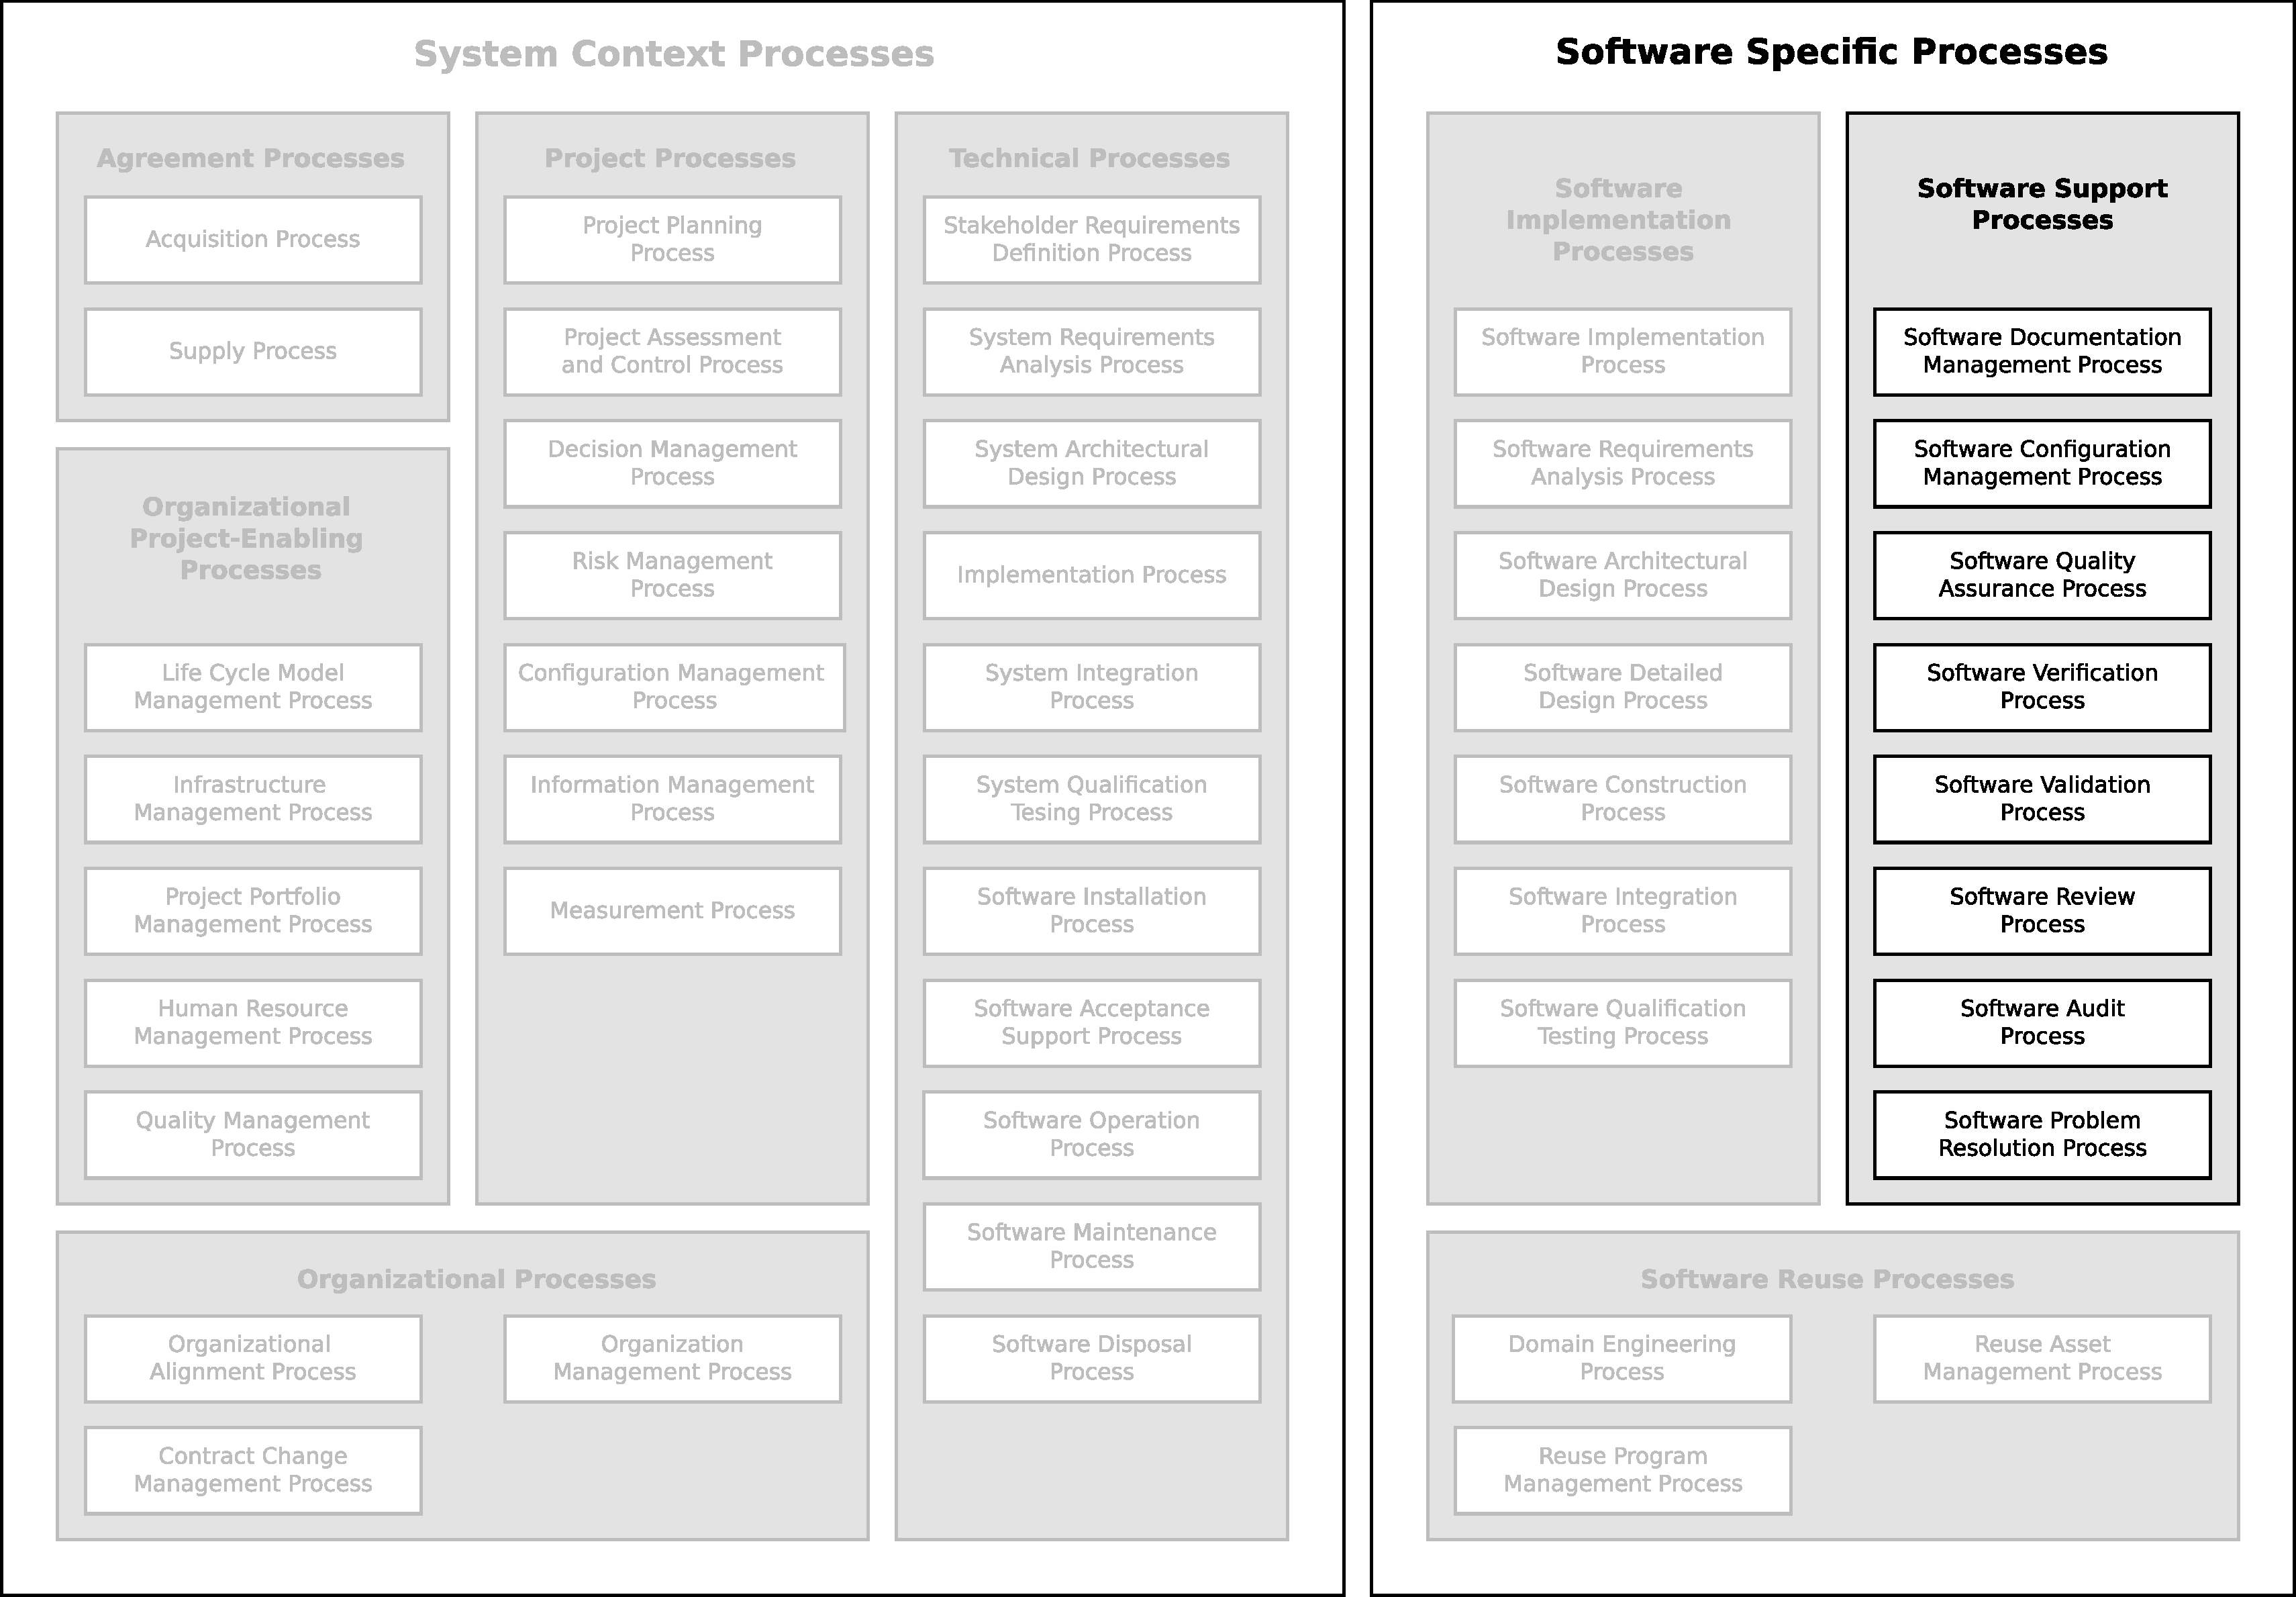
\includegraphics[width=15cm,keepaspectratio]{figures/life-cycle-process-groups-software-support-processes.pdf}
			\caption{Software Support Processes}
			\label{fig:software_support_processes}
		\end{figure}

		\begin{adjustwidth}{1em}{0pt}
			
			{\bf Note}: The support processes listed in this section are specific to software and are labeled \nameref{subsec:software_support_processes}. Although they play an integral role in assisting the \nameref{proc:software_implementation_process}, the Software Support Processes may also provide services to other processes, e.g., the \nameref{subsec:agreement_processes}, \nameref{proc:system_qualification_testing_process}, \nameref{proc:software_acceptance_support_process}, \nameref{proc:software_operation_process}, and \nameref{proc:software_maintenance_process}.

			\begin{compactitem}

				\item \ref{proc:software_documentation_management_process} - \nameref{proc:software_documentation_management_process}

				\item \ref{proc:software_configuration_management_process} - \nameref{proc:software_configuration_management_process}

				\item \ref{proc:software_quality_assurance_process} - \nameref{proc:software_quality_assurance_process}

				\item \ref{proc:software_verification_process} - \nameref{proc:software_verification_process}

				\item \ref{proc:software_validation_process} - \nameref{proc:software_validation_process}

				\item \ref{proc:software_review_process} - \nameref{proc:software_review_process}

				\item \ref{proc:software_audit_process} - \nameref{proc:software_audit_process}

				\item \ref{proc:software_problem_resolution_process} - \nameref{proc:software_problem_resolution_process}

			\end{compactitem}

		\end{adjustwidth}

		\newpage
		\subsubsection{SOFTWARE DOCUMENTATION MANAGEMENT PROCESS\label{proc:software_documentation_management_process}}

			\subsubsubsection{PURPOSE}
			\begin{adjustwidth}{2em}{0pt} 

				The purpose of the \nameref{proc:software_documentation_management_process} is to develop and maintain the recorded software information produced by a process.

			\end{adjustwidth}

			\subsubsubsection{OUTCOMES}
			\begin{adjustwidth}{2em}{0pt} 

				\begin{compactitem}

					\item a strategy identifying the documentation to be produced during the life cycle of the software product or service is developed;

					\item the standards to be applied for the development of the software documentation are identified;

					\item documentation to be produced by the process or project is identified;

					\item the content and purpose of all documentation is specified, reviewed and approved;

					\item documentation is developed and made available in accordance with identified standards; and

					\item documentation is maintained in accordance with defined criteria.

				\end{compactitem}

			\end{adjustwidth}

			\subsubsubsection{ACTIVITIES AND TASKS}
			\begin{adjustwidth}{2em}{0pt} 

				\begin{compactenum}

					\item {\bf Process Implementation}:
					\begin{compactenum}

						\item A plan, identifying the documents to be produced during the life cycle of the software product shall be developed, documented, and implemented. For identified documentation, the following shall be addressed:

						\begin{compactenum}

							\item Title or name.

							\item Purpose and content.

							\item Intended audience.

							\item Procedures and responsibilities for inputs, development, review, modification, approval, production,
							storage, distribution, maintenance, and configuration management.

							\item Schedule for intermediate and final versions.

						\end{compactenum}

					\end{compactenum}

					\item {\bf Design and Development}:
					\begin{compactenum}

						\item Each identified document shall be designed in accordance with applicable documentation standards for medium, format, content description, page numbering, figure/table placement, proprietary/security marking, packaging, and other presentation items.

						\item The source and appropriateness of input data for the documents shall be confirmed. Automated documentation support tools may be used.

						\item The prepared documents shall be reviewed and edited for format, technical content, and presentation style against their documentation standards. They shall be approved for adequacy by authorized personnel prior to issue.

					\end{compactenum}

					\item {\bf Production}:
					\begin{compactenum}

						\item The documents shall be produced and provided in accordance with the plan. Production and distribution of documents may use paper, electronic, or other media. Master materials shall be stored in accordance with requirements for record retention, security, maintenance, and backup.

						\item Controls shall be established in accordance with the \nameref{proc:software_configuration_management_process}.

					\end{compactenum}

					\item {\bf Maintenance}:
					\begin{compactenum}

						\item The tasks of the \nameref{proc:software_maintenance_process}, that are required when documentation is to be modified, shall be performed. For those documents that are under configuration management, modifications shall be managed in accordance with the \nameref{proc:software_configuration_management_process}.

					\end{compactenum}

				\end{compactenum}

			\end{adjustwidth}

		\newpage
		\subsubsection{SOFTWARE CONFIGURATION MANAGEMENT PROCESS\label{proc:software_configuration_management_process}}

			\subsubsubsection{PURPOSE}
			\begin{adjustwidth}{2em}{0pt} 

				The purpose of the \nameref{proc:software_configuration_management_process} is to establish and maintain the integrity of the software items of a process or project and make them available to concerned parties.

			\end{adjustwidth}

			\subsubsubsection{OUTCOMES}
			\begin{adjustwidth}{2em}{0pt} 

				\begin{compactitem}

					\item a software configuration management strategy is developed;

					\item items generated by the process or project are identified, defined and baselined;

					\item modifications and releases of the items are controlled;

					\item modifications and releases are made available to affected parties;

					\item the status of the items and modifications are recorded and reported;

					\item the completeness and consistency of the items is ensured; and

					\item the storage, handling and delivery of the items are controlled.

				\end{compactitem}

			\end{adjustwidth}

			\subsubsubsection{ACTIVITIES AND TASKS}
			\begin{adjustwidth}{2em}{0pt} 

				\begin{compactenum}

					\item {\bf Process Implementation}:

					\begin{compactenum}

						\item A software configuration management plan shall be developed. The plan shall describe: the configuration management activities; procedures and schedule for performing these activities; the organization(s) responsible for performing these activities; and their relationship with other organizations, such as software development or maintenance. The plan shall be documented and implemented.

					\end{compactenum}

					\item {\bf Configuration Identification}:

					\begin{compactenum}

						\item A scheme shall be established for identification of software items and their versions to be controlled for the project. For each software item and its versions, the following shall be identified: the documentation that establishes the baseline; the version references; and other identification details.

					\end{compactenum}

					\item {\bf Configuration Control}:

					\begin{compactenum}

						\item The following shall be performed: identification and recording of change requests; analysis and evaluation of the changes; approval or disapproval of the request; and implementation, verification, and release of the modified software item. An audit trail shall exist, whereby each modification, the reason for the modification, and authorization of the modification can be traced. Control and audit of all accesses to the controlled software items that handle safety or security critical functions shall be performed.

					\end{compactenum}

					\item {\bf Configuration Status Accounting}:

					\begin{compactenum}

						\item Management records and status reports that show the status and history of controlled software items, including baselines shall be prepared. Status reports should include the number of changes for a project, latest software item versions, release identifiers, the number of releases, and comparisons of releases.

					\end{compactenum}

					\item {\bf Configuration Evaluation}:

					\begin{compactenum}

						\item The following shall be determined and ensured: the functional completeness of the software items against their requirements and the physical completeness of the software items (whether their design and code reflect an up-to-date technical description).

					\end{compactenum}

					\item {\bf Release Management and Delivery}:

					\begin{compactenum}

						\item The release and delivery of software products and documentation shall be formally controlled. Master copies of code and documentation shall be maintained for the life of the software product. The code and documentation that contain safety or security critical functions shall be handled, stored, packaged, and delivered in accordance with the policies of the organizations involved.

					\end{compactenum}

				\end{compactenum}

			\end{adjustwidth}

		\newpage
		\subsubsection{SOFTWARE QUALITY ASSURANCE PROCESS\label{proc:software_quality_assurance_process}}

			\subsubsubsection{PURPOSE}
			\begin{adjustwidth}{2em}{0pt} 

				The purpose of the \nameref{proc:software_quality_assurance_process} is to provide assurance that work products and processes comply with predefined provisions and plans.

			\end{adjustwidth}

			\subsubsubsection{OUTCOMES}
			\begin{adjustwidth}{2em}{0pt} 

				\begin{compactitem}

					\item a strategy for conducting quality assurance is developed;

					\item evidence of software quality assurance is produced and maintained;

					\item problems and/or non-conformance with requirements are identified and recorded; and

					\item adherence of products, processes and activities to the applicable standards, procedures and requirements are verified.

				\end{compactitem}

			\end{adjustwidth}

			\subsubsubsection{ACTIVITIES AND TASKS}
			\begin{adjustwidth}{2em}{0pt} 

				\begin{compactenum}

					\item {\bf Process Implementation}:

					\begin{compactenum}

						\item A quality assurance process suited to the project shall be established. The objectives of the quality assurance process shall be to assure that the software products and the processes employed for providing those software products comply with their established requirements and adhere to their established plans.

						\item The quality assurance process should be coordinated with the related \nameref{proc:software_verification_process}, \nameref{proc:software_validation_process}, \nameref{proc:software_review_process}, and \nameref{proc:software_audit_process}.

						\item A plan for conducting the quality assurance process activities and tasks shall be developed, documented, implemented, and maintained for the life of the contract. The plan shall include the following:

						\begin{compactenum}

							\item Quality standards, methodologies, procedures, and tools for performing the quality assurance activities (or their references in organization's official documentation).

							\item Procedures for contract review and coordination thereof.

							\item Procedures for identification, collection, filing, maintenance, and disposition of quality records.

							\item Resources, schedule, and responsibilities for conducting the quality assurance activities.

							\item Selected activities and tasks from supporting processes, such as the \nameref{proc:software_verification_process}, \nameref{proc:software_validation_process}, \nameref{proc:software_review_process}, \nameref{proc:software_audit_process}, and \nameref{proc:software_problem_resolution_process}.

						\end{compactenum}

							\item Scheduled and on-going quality assurance activities and tasks shall be executed. When problems or non-conformances with contract requirements are detected, they shall be documented and serve as input to the \nameref{proc:software_problem_resolution_process}. Records of these activities and tasks, their execution, problems, and problem resolutions shall be prepared and maintained.

							\item Records of quality assurance activities and tasks shall be made available to the acquirer as specified in the contract.

							\item It shall be assured that persons responsible for assuring compliance with the contract requirements have the organizational freedom, resources, and authority to permit objective evaluations and to initiate, effect, resolve, and verify problem resolutions.

					\end{compactenum}

					\item {\bf Product Assurance}:

					\begin{compactenum}

						\item It shall be assured that all the plans required by the contract are documented, comply with the contract, are mutually consistent, and are being executed as required.

						\item It shall be assured that software products and related documentation comply with the contract and adhere to the plans.

						\item In preparation for the delivery of the software products, it shall be assured that they have fully satisfied their contractual requirements and are acceptable to the acquirer.

					\end{compactenum}

					\item {\bf Process Assurance}:

					\begin{compactenum}

						\item It shall be assured that those software life cycle processes (supply, development, operation, maintenance, and support processes including quality assurance) employed for the project comply with the contract and adhere to the plans.

						\item It shall be assured that the internal software engineering practices, development environment, test environment, and libraries comply with the contract.

						\item It shall be assured that applicable prime-contract requirements are passed down to the subcontractor, and that the subcontractor's software products satisfy prime-contract requirements.

						\item It shall be assured that the acquirer and other parties are provided the required support and cooperation in accordance with the contract, negotiations, and plans.

						\item It should be assured that software product and process measurements are in accordance with established standards and procedures.

						\item It shall be assured that the staff assigned have the skill and knowledge needed to meet the requirements of the project and receive any necessary training.

					\end{compactenum}

				\end{compactenum}

			\end{adjustwidth}

		\newpage
		\subsubsection{SOFTWARE VERIFICATION PROCESS\label{proc:software_verification_process}}

			\subsubsubsection{PURPOSE}
			\begin{adjustwidth}{2em}{0pt} 

				The purpose of the \nameref{proc:software_verification_process} is to confirm that each software work product and/or service of a process or project properly reflects the specified requirements.

			\end{adjustwidth}

			\subsubsubsection{OUTCOMES}
			\begin{adjustwidth}{2em}{0pt} 

				\begin{compactitem}

					\item a verification strategy is developed and implemented;

					\item criteria for verification of all required software work products is identified;

					\item required verification activities are performed;

					\item defects are identified and recorded; and

					\item results of the verification activities are made available to the customer and other involved parties.

				\end{compactitem}

			\end{adjustwidth}

			\subsubsubsection{ACTIVITIES AND TASKS}
			\begin{adjustwidth}{2em}{0pt} 

				\begin{compactenum}

					\item {\bf Process Implementation}:

					\begin{compactenum}

						\item A determination shall be made if the project warrants a verification effort and the degree of organizational independence of that effort needed. The project requirements shall be analyzed for criticality. Criticality may be gauged in terms of:

						\begin{compactenum}

							\item The potential of an undetected error in a system or software requirement for causing death or personal injury, mission failure, or financial or catastrophic equipment loss or damage.

							\item The maturity of and risks associated with the software technology to be used.

							\item Availability of funds and resources.

						\end{compactenum}

						\item If the project warrants a verification effort, a verification process shall be established to verify the software product.

						\item If the project warrants an independent verification effort, a qualified organization responsible for conducting the verification shall be selected. This organization shall be assured of the independence and authority to perform the verification activities.

						\item Based upon the scope, magnitude, complexity, and criticality analysis above, target life cycle activities and software products requiring verification shall be determined. Verification activities and tasks defined in the \nameref{proc:software_verification_process}, including associated methods, techniques, and tools for performing the tasks, shall be selected for the target life cycle activities and software products.

						\item Based upon the verification tasks as determined, a verification plan shall be developed and documented. The plan shall address the life cycle activities and software products subject to verification, the required verification tasks for each life cycle activity and software product, and related resources, responsibilities, and schedule. The plan shall address procedures for forwarding verification reports to the acquirer and other involved organizations.

						\item The verification plan shall be implemented. Problems and non-conformances detected by the verification effort shall be entered into the \nameref{proc:software_problem_resolution_process}. All problems and non-conformances shall be resolved. Results of the verification activities shall be made available to the acquirer and other involved organizations.

					\end{compactenum}

					\item {\bf Requirements Verification}:

					\begin{compactenum}

						\item The system requirements are consistent, feasible, and testable.

						\item The system requirements have been appropriately allocated to hardware items, software items, and manual operations according to design criteria.

						\item The software requirements are consistent, feasible, testable, and accurately reflect system requirements.

						\item The software requirements related to safety, security, and criticality are correct as shown by suitably rigorous methods.

					\end{compactenum}

					\item {\bf Design Verification}:

					\begin{compactenum}

						\item The design is correct and consistent with and traceable to requirements.

						\item The design implements proper sequence of events, inputs, outputs, interfaces, logic flow, allocation of timing and sizing budgets, and error definition, isolation, and recovery.

						\item Selected design can be derived from requirements.

						\item The design implements safety, security, and other critical requirements correctly as shown by suitably rigorous methods.

					\end{compactenum}

					\item {\bf Code Verification}:

					\begin{compactenum}

						\item The code is traceable to design and requirements, testable, correct, and compliant with requirements and coding standards.

						\item The code implements proper event sequence, consistent interfaces, correct data and control flow, completeness, appropriate allocation timing and sizing budgets, and error definition, isolation, and recovery.

						\item Selected code can be derived from design or requirements.

						\item The code implements safety, security, and other critical requirements correctly as shown by suitably rigorous methods.

					\end{compactenum}

					\item {\bf Integration Verification}:

					\begin{compactenum}

						\item The software components and units of each software item have been completely and correctly integrated into the software item.

						\item The hardware items, software items, and manual operations of the system have been completely and correctly integrated into the system.

						\item The integration tasks have been performed in accordance with an integration plan.

					\end{compactenum}

					\item {\bf Documentation Verification}:

					\begin{compactenum}

						\item The documentation is adequate, complete, and consistent.

						\item Documentation preparation is timely.

						\item Configuration management of documents follows specified procedures.

					\end{compactenum}

				\end{compactenum}

			\end{adjustwidth}

		\newpage
		\subsubsection{SOFTWARE VALIDATION PROCESS\label{proc:software_validation_process}}

			\subsubsubsection{PURPOSE}
			\begin{adjustwidth}{2em}{0pt} 
				
				The purpose of the \nameref{proc:software_validation_process} is to confirm that the requirements for a specific intended use of the software work product are fulfilled.

			\end{adjustwidth}

			\subsubsubsection{OUTCOMES}
			\begin{adjustwidth}{2em}{0pt} 

				\begin{compactitem}

					\item a validation strategy is developed and implemented;

					\item criteria for validation of all required work products are identified;

					\item required validation activities are performed;

					\item problems are identified and recorded;

					\item evidence is provided that the software work products as developed are suitable for their intended use; and

					\item results of the validation activities are made available to the customer and other involved parties.

				\end{compactitem}

			\end{adjustwidth}

			\subsubsubsection{ACTIVITIES AND TASKS}
			\begin{adjustwidth}{2em}{0pt} 

				\begin{compactenum}

					\item {\bf Process Implementation}:

					\begin{compactenum}

						\item A determination shall be made if the project warrants a validation effort and the degree of organizational independence of that effort needed.

						\item If the project warrants a validation effort, a validation process shall be established to validate the system or software product. Validation tasks defined below, including associated methods, techniques, and tools for performing the tasks, shall be selected.

						\item If the project warrants an independent effort, a qualified organization responsible for conducting the effort shall be selected. The conductor shall be assured of the independence and authority to perform the validation tasks.

						\item A validation plan shall be developed and documented. The plan shall include, but is not limited to, the following:

						\begin{compactenum}

							\item Items subject to validation.

							\item Validation tasks to be performed.

							\item Resources, responsibilities, and schedule for validation.

							\item Procedures for forwarding validation reports to the acquirer and other parties.

						\end{compactenum}

						\item The validation plan shall be implemented. Problems and non-conformances detected by the validation effort shall be entered into the \nameref{proc:software_problem_resolution_process}. All problems and non-conformances shall be resolved. Results of the validation activities shall be made available to the acquirer and other involved organizations.

					\end{compactenum}

					\item {\bf Validation}:

					\begin{compactenum}

						\item Prepare selected test requirements, test cases, and test specifications for analyzing test results.

						\item Ensure that these test requirements, test cases, and test specifications reflect the particular requirements for the specific intended use.

						\item Conduct the tests in the previous two points, including:

						\begin{compactenum}

							\item Testing with stress, boundary, and singular inputs;

							\item Testing the software product for its ability to isolate and minimize the effect of errors; that is, graceful degradation upon failure, request for operator assistance upon stress, boundary, and singular conditions;

							\item Testing that representative users can successfully achieve their intended tasks using the software product.

						\end{compactenum}
						
						\item Validate that the software product satisfies its intended use.

						\item Test the software product as appropriate in selected areas of the target environment.

					\end{compactenum}

				\end{compactenum}

			\end{adjustwidth}

		\newpage
		\subsubsection{SOFTWARE REVIEW PROCESS\label{proc:software_review_process}}

			\subsubsubsection{PURPOSE}
			\begin{adjustwidth}{2em}{0pt} 

				The purpose of the \nameref{proc:software_review_process} is to maintain a common understanding with the stakeholders of the progress against the objectives of the agreement and what should be done to help ensure development of a product that satisfies the stakeholders. 

				Software reviews are at both project management and technical levels and are held throughout the life of the project.

			\end{adjustwidth}

			\subsubsubsection{OUTCOMES}
			\begin{adjustwidth}{2em}{0pt} 

				\begin{compactitem}

					\item management and technical reviews are held based on the needs of the project;

					\item the status and products of an activity of a process are evaluated through review activities;

					\item review results are made known to all affected parties;

					\item action items resulting from reviews are tracked to closure; and

					\item risks and problems are identified and recorded.

				\end{compactitem}

			\end{adjustwidth}

			\subsubsubsection{ACTIVITIES AND TASKS}
			\begin{adjustwidth}{2em}{0pt} 

				\begin{compactenum}

					\item {\bf Process Implementation}:

					\begin{compactenum}

						\item Periodic reviews shall be held at predetermined milestones as specified in the project plan(s). Stakeholders should determine the need for any ad hoc reviews in which agreeing parties may participate.

						\item All resources that are required to conduct the reviews shall be provided. These resources include personnel, location, facilities, hardware, software, and tools.

						\item The parties that participate in a review should agree on the following items at each review: meeting agenda, software products (results of an activity) and problems to be reviewed; scope and procedures; and entry and exit criteria for the review.

						\item Problems detected during the reviews shall be recorded and entered into the \nameref{proc:software_problem_resolution_process} as required.

						\item The review results shall be documented and distributed. This communication includes adequacy of review (for example, approval, disapproval, or contingent approval) of the review results.

						\item Participating parties shall agree on the outcome of the review and any action item responsibilities and closure criteria.

					\end{compactenum}

					\item {\bf Process Management Reviews}:

					\begin{compactenum}

						\item Project status shall be evaluated relative to the applicable project plans, schedules, standards, and guidelines. The outcome of the review should be considered by appropriate management and should provide for the following:

						\begin{compactenum}

							\item Making activities progress according to plan, based on an evaluation of the activity or software product
							status.

							\item Maintaining global control of the project through adequate allocation of resources.

							\item Changing project direction or determining the need for alternate planning.

							\item Evaluating and managing the risk issues that may jeopardize the success of the project.

						\end{compactenum}

					\end{compactenum}

					\item {\bf Technical Reviews}:

					\begin{compactenum}

						\item Technical reviews shall be held to evaluate the software products or services under consideration and provide evidence that:

						\begin{compactenum}

							\item They are complete.

							\item They comply with their standards and specifications.

							\item Changes to them are properly implemented and affect only those areas identified by the \nameref{proc:configuration_management_process}.

							\item They are adhering to applicable schedules.

							\item They are ready for the next planned activity.

							\item The development, operation, or maintenance is being conducted according to the plans, schedules, standards, and guidelines of the project.

						\end{compactenum}

					\end{compactenum}

				\end{compactenum}

			\end{adjustwidth}

		\newpage
		\subsubsection{SOFTWARE AUDIT PROCESS\label{proc:software_audit_process}}

			\subsubsubsection{PURPOSE}
			\begin{adjustwidth}{2em}{0pt} 

				The purpose of the \nameref{proc:software_audit_process} is to independently determine compliance of selected products and processes with the requirements, plans and agreement, as appropriate.

			\end{adjustwidth}

			\subsubsubsection{OUTCOMES}
			\begin{adjustwidth}{2em}{0pt} 

				\begin{compactitem}

					\item an audit strategy is developed and implemented;

					\item compliance of selected software work products and/or services or processes with requirements, plans and agreement is determined according to the audit strategy;

					\item audits are conducted by an appropriate independent party; and

					\item problems detected during an audit are identified and communicated to those responsible for corrective action, and resolution.

				\end{compactitem}

			\end{adjustwidth}

			\subsubsubsection{ACTIVITIES AND TASKS}
			\begin{adjustwidth}{2em}{0pt} 

				\begin{compactenum}

					\item {\bf Process Implementation}:

					\begin{compactenum}

						\item Auditing personnel shall not have any direct responsibility for the software products and activities they audit.

						\item All resources required to conduct the audits shall be agreed by the parties. These resources include support personnel, location, facilities, hardware, software, and tools.

						\item The parties should agree on the following items at each audit: agenda; software products (and results of an activity) to be reviewed; audit scope and procedures; and entry and exit criteria for the audit.

						\item Problems detected during the audits shall be recorded and entered into the \nameref{proc:software_problem_resolution_process} as required.

						\item After completing an audit, the audit results shall be documented and provided to the audited party. The audited party shall acknowledge to the auditing party any problems found in the audit and related problem resolutions planned.

						\item The parties shall agree on the outcome of the audit and any action item responsibilities and closure criteria.

					\end{compactenum}

					\item {\bf Software Audit}:

					\begin{compactenum}

						\item Software audits shall be conducted to ensure that:

						\begin{compactenum}

							\item As coded, software products (such as a software item) reflect the design documentation.

							\item The acceptance review and testing requirements prescribed by the documentation are adequate for the acceptance of the software products.

							\item Test data comply with the specification.

							\item Software products were successfully tested and meet their specifications.

							\item Test reports are correct and discrepancies between actual and expected results have been resolved.

							\item User documentation complies with standards as specified.

							\item Activities have been conducted according to applicable requirements, plans, and contract.

							\item The costs and schedules adhere to the established plans.

						\end{compactenum}

					\end{compactenum}

				\end{compactenum}

			\end{adjustwidth}

		\newpage
		\subsubsection{SOFTWARE PROBLEM RESOLUTION PROCESS\label{proc:software_problem_resolution_process}}

			\subsubsubsection{PURPOSE}
			\begin{adjustwidth}{2em}{0pt} 

				The purpose of the \nameref{proc:software_problem_resolution_process} is to ensure that all discovered problems are identified, analyzed, managed and controlled to resolution.

			\end{adjustwidth}

			\subsubsubsection{OUTCOMES}
			\begin{adjustwidth}{2em}{0pt} 

				\begin{compactitem}

					\item a problem management strategy is developed;

					\item problems are recorded, identified and classified;

					\item problems are analyzed and assessed to identify acceptable solution(s);

					\item problem resolution is implemented;

					\item problems are tracked to closure; and

					\item the status of all problems reported is known.

				\end{compactitem}

			\end{adjustwidth}

			\subsubsubsection{ACTIVITIES AND TASKS}
			\begin{adjustwidth}{2em}{0pt} 

				\begin{compactenum}

					\item {\bf Process Implementation}:

					\begin{compactenum}

						\item A problem resolution process shall be established for handling all problems (including non-conformances) detected in the software products and activities. The process shall comply with the following requirements:

						\begin{compactenum}

							\item The process shall be closed-loop, ensuring that: all detected problems are promptly reported and entered into the Problem Resolution Process; action is initiated on them; relevant parties are advised of the existence of the problem as appropriate; causes are identified, analyzed, and, where possible, eliminated; resolution and disposition are achieved; status is tracked and reported; and records of the problems are maintained as stipulated in the contract.

							\item The process should contain a scheme for categorizing and prioritizing the problems. Each problem should be classified by the category and priority to facilitate trend analysis and problem resolution.

							\item Analysis shall be performed to detect trends in the problems reported.

							\item Problem resolutions and dispositions shall be evaluated: to evaluate that problems have been resolved, adverse trends have been reversed, and changes have been correctly implemented in the appropriate software products and activities; and to determine whether additional problems have been introduced.

						\end{compactenum}

					\end{compactenum}

					\item {\bf Problem Resolution}:

					\begin{compactenum}

						\item When problems (including non-conformances) have been detected in a software product or an activity, a problem report shall be prepared to describe each problem detected. The problem report shall be used as part of the closed-loop process described above: from detection of the problem, through investigation, analysis and resolution of the problem and its cause, and onto trend detection across problems.

					\end{compactenum}

				\end{compactenum}

			\end{adjustwidth}


	\newpage 
	\subsection{SOFTWARE REUSE PROCESSES\label{subsec:software_reuse_processes}}

		\begin{figure}[h]
			\centering
			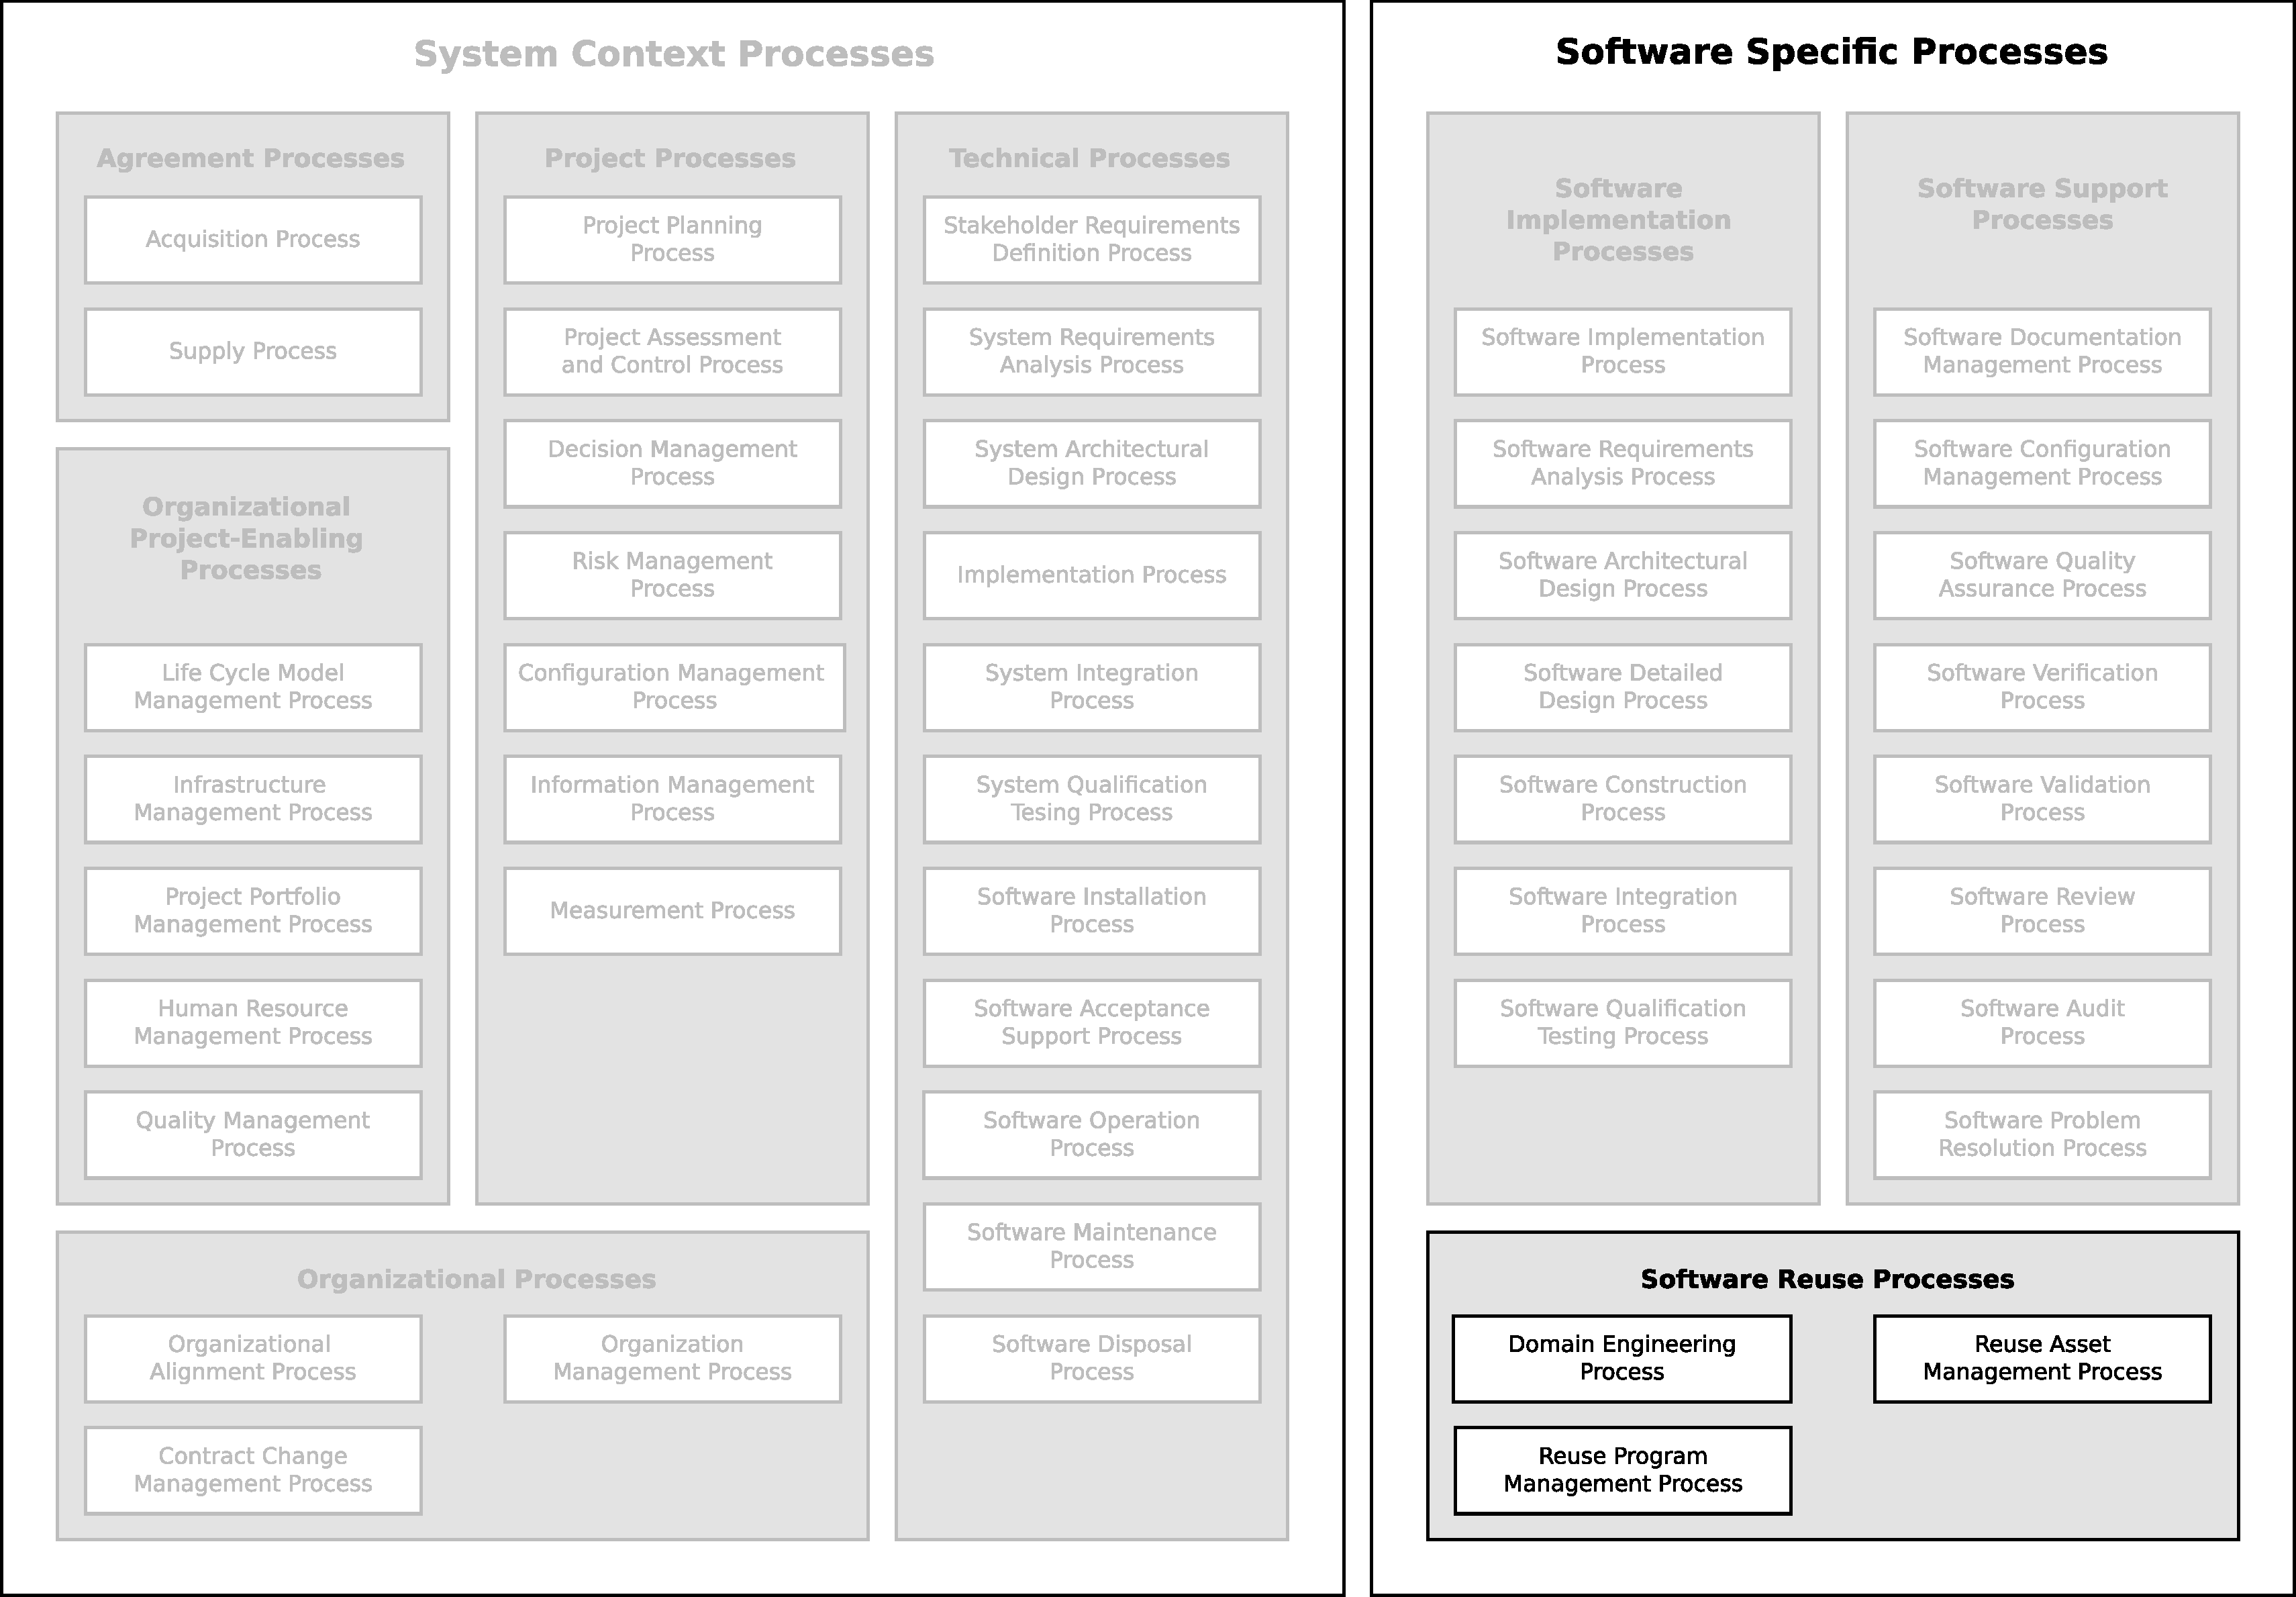
\includegraphics[width=15cm,keepaspectratio]{figures/life-cycle-process-groups-software-reuse-processes.pdf}
			\caption{Software Reuse Processes}
			\label{fig:software_reuse_processes}
		\end{figure}

		\begin{adjustwidth}{1em}{0pt}

			The \nameref{subsec:software_reuse_processes} consist of three processes that support an organization's ability to reuse software items across project boundaries. These processes are unique because, by their nature, they operate outside the bounds of any particular project.

			\begin{compactitem}
				\item \ref{proc:domain_engineering_process} \nameref{proc:domain_engineering_process}
				\item \ref{proc:reuse_asset_management_process} \nameref{proc:reuse_asset_management_process}
				\item \ref{proc:reuse_program_management_process} \nameref{proc:reuse_program_management_process}
			\end{compactitem}

		\end{adjustwidth}

		\newpage
		\subsubsection{DOMAIN ENGINEERING PROCESS\label{proc:domain_engineering_process}}

			\subsubsubsection{PURPOSE}
			\begin{adjustwidth}{2em}{0pt} 

				The purpose of the \nameref{proc:domain_engineering_process} is to develop and maintain domain models, domain architectures and assets for the domain.

			\end{adjustwidth}

			\subsubsubsection{OUTCOMES}
			\begin{adjustwidth}{2em}{0pt} 

				\begin{compactitem}

					\item the representation forms for the domain models and the domain architectures are selected;

					\item the boundaries of the domain and its relationships to other domains are established;

					\item a domain model that captures the essential common and different features, capabilities, concepts, and functions in the domain are developed;

					\item a domain architecture describing the family of systems within the domain, including their commonalities and variabilities, is developed;

					\item assets belonging to the domain are specified;

					\item assets belonging to the domain are acquired or developed and maintained throughout their life cycles; and

					\item the domain models and architectures are maintained throughout their life cycles.

				\end{compactitem}

			\end{adjustwidth}

			\subsubsubsection{ACTIVITIES AND TASKS}
			\begin{adjustwidth}{2em}{0pt} 

				\begin{compactenum}

					\item {\bf Process Implementation}:

					\begin{compactenum}

						\item The domain engineer shall create and execute a domain engineering plan.

						\item The domain engineer shall select the form(s) of representation to be used for domain architectures and models.

						\item The domain engineer shall establish procedures for receiving, resolving, and providing feedback to the asset manager whenever problems or change requests occur for assets developed by the domain engineer.

					\end{compactenum}

					\item {\bf Domain Analysis}:

					\begin{compactenum}

						\item The domain engineer shall define the boundaries of the domain and the relationships between this domain and other domains.

						\item The domain engineer shall identify the current and anticipated needs of stakeholders of software products within this domain.

						\item The domain engineer shall build the domain models using the representation forms selected in the Process Implementation Activity for this process.

						\item The domain engineer shall construct a vocabulary that provides the terminology to describe the important domain concepts and the relationships among similar or common assets of the domain.

						\item The domain engineer shall classify and document the domain models.

						\item The domain engineer shall evaluate the domain models and domain vocabulary in accordance with the provisions of the modeling technique selected and in accordance with the organization’s asset acceptance and certification procedures.

						\item The domain engineer shall conduct domain analysis review(s). Software developers, asset managers, domain experts, and users shall be included in the reviews.

						\item The domain engineer shall submit domain models to the asset manager.

					\end{compactenum}

					\item {\bf Domain Design}:

					\begin{compactenum}

						\item The domain engineer shall create and document the domain architecture, consistent with the domain model and following the organization’s standards.

						\item The domain architecture shall be evaluated in accordance with the provisions of the architecture design technique selected and the organization’s asset acceptance and certification procedures.

						\item For each entity selected to be designed for reuse, the domain engineer shall develop and document an asset specification.

						\item For each asset specified, the specification shall be evaluated in accordance with the organization’s asset acceptance and certification procedures.

						\item The domain engineer shall conduct domain design review(s). Software developers, domain experts, and asset managers shall be included in the reviews.

						\item The domain engineer shall submit the domain architecture to the asset manager.

					\end{compactenum}

					\item {\bf Asset Provision}:

					\begin{compactenum}

						\item The domain engineer shall obtain the asset by acquisition or by development.

						\item The domain engineer shall document and classify the asset.

						\item The domain engineer shall evaluate the asset in accordance with the organization’s asset acceptance and certification procedures.

						\item The domain engineer shall conduct asset review(s). Software developers and asset managers shall be included in the reviews.

						\item The domain engineer shall submit the asset to the asset manager.

					\end{compactenum}

					\item {\bf Asset Maintenance}:

					\begin{compactenum}

						\item When analyzing requests for asset modification and choosing implementation options, the domain engineer shall consider:

						\begin{compactenum}

							\item Conformance with the domain models and the domain architecture;

							\item Impact on the systems and software products that use the asset;

							\item Impact on future users of the asset;

							\item Impact on the reusability of the asset.

						\end{compactenum}

					\end{compactenum}

				\end{compactenum}

			\end{adjustwidth}

		\newpage
		\subsubsection{REUSE ASSET MANAGEMENT PROCESS\label{proc:reuse_asset_management_process}}

			\subsubsubsection{PURPOSE}
			\begin{adjustwidth}{2em}{0pt} 

				The purpose of the \nameref{proc:reuse_asset_management_process} is to manage the life of reusable assets from conception to retirement.

			\end{adjustwidth}

			\subsubsubsection{OUTCOMES}
			\begin{adjustwidth}{2em}{0pt} 

				\begin{compactitem}

					\item an asset management strategy is documented;

					\item an asset classification scheme is established;

					\item criteria for asset acceptance, certification and retirement are defined;

					\item an asset storage and retrieval mechanism is operated;

					\item the use of assets is recorded;

					\item changes to the assets are controlled, and

					\item users of assets are notified of problems detected, modifications made, new versions created and deletion of assets from the storage and retrieval mechanism.

				\end{compactitem}

			\end{adjustwidth}

			\subsubsubsection{ACTIVITIES AND TASKS}
			\begin{adjustwidth}{2em}{0pt} 

				\begin{compactenum}

					\item {\bf Process Implementation}:

					\begin{compactenum}

						\item The asset manager shall create an asset management plan to define the resources and procedures for managing assets.

						\item The asset manager shall execute the plan.

						\item The asset management plan shall be reviewed in accordance with the Software Review Process. Domain engineers and reuse program administrators shall be included in the review.

					\end{compactenum}

					\item {\bf Asset Storage and Retrieval Definition}:

					\begin{compactenum}

						\item The asset manager shall implement and maintain an asset storage and retrieval mechanism.

						\item The asset manager should develop, document, and maintain a classification scheme to be used in classifying the assets.

						\item The asset manager shall conduct review(s) of the asset storage and retrieval mechanism in accordance with the Software Review Process. Reuse program administrators and domain engineers shall be included in the review(s).

					\end{compactenum}

					\item {\bf Asset Management and Control}:

					\begin{compactenum}

						\item For each asset submitted to the asset manager, the asset shall be evaluated based on the asset acceptance and certification criteria.

						\item For each asset accepted, it shall be made available for reuse through the asset storage and retrieval mechanism.

						\item The asset shall be classified in accordance with the reuse classification scheme, if any exists.

						\item The asset manager shall perform configuration management for the asset using the Software Configuration Management Process.

						\item The asset manager shall keep track of each reuse of the asset and report to the domain engineer information about actual reuses of the asset.

						\item The asset manager shall forward asset modification requests and problem reports received from asset reusers to the domain engineer for review and correction/modification plans and actions.

						\item The asset manager shall monitor and record these asset requests/reports and the subsequent actions taken.

						\item The asset manager shall notify all asset reusers, and the domain engineer, of the problems detected in the asset, modifications made to the asset, new versions of the asset, and deletion of the asset from the asset storage and retrieval mechanism.

						\item The asset manager shall retire assets from the asset storage and retrieval mechanism according to the asset retirement procedures and criteria.

					\end{compactenum}

				\end{compactenum}

			\end{adjustwidth}

		\newpage
		\subsubsection{REUSE PROGRAM MANAGEMENT PROCESS\label{proc:reuse_program_management_process}}

			\subsubsubsection{PURPOSE}
			\begin{adjustwidth}{2em}{0pt} 

				The purpose of the \nameref{proc:reuse_program_management_process} is to plan, establish, manage, control, and monitor an organization's reuse program and to systematically exploit reuse opportunities.

			\end{adjustwidth}

			\subsubsubsection{OUTCOMES}
			\begin{adjustwidth}{2em}{0pt} 

				\begin{compactitem}

					\item the organization's reuse strategy, including its purpose, scope, goals and objectives, is defined;

					\item the domains for potential reuse opportunities are identified;

					\item the organization's systematic reuse capability is assessed;

					\item the reuse potential of each domain is assessed;

					\item reuse proposals are evaluated to ensure the reuse product is suitable for the proposed application;

					\item the reuse strategy is implemented in the organization;

					\item feedback, communication, and notification mechanisms that operate between affected parties are established; and

					\item the reuse program is monitored and evaluated.

				\end{compactitem}

			\end{adjustwidth}

			\subsubsubsection{ACTIVITIES AND TASKS}
			\begin{adjustwidth}{2em}{0pt} 

				\begin{compactenum}

					\item {\bf Initiation}:

					\begin{compactenum}

						\item The reuse program for an organization shall be initiated by establishing the organization’s reuse strategy that includes its reuse goals, purposes, objectives, and scope.

						\item A reuse sponsor should be named.

						\item Reuse program participants shall be identified and their roles shall be assigned.

						\item A reuse steering function shall be established to assume the authority and responsibility for the organization’s reuse program.

						\item A reuse program support function shall be established.

					\end{compactenum}

					\item {\bf Domain Identification}:

					\begin{compactenum}

						\item The reuse program administrator, aided by the appropriate manager, domain engineers, users, and software developers, shall identify and document the domains in which to investigate reuse opportunities or in which the organization intends to practice reuse.

						\item The reuse program administrator, aided by the appropriate managers, domain engineers, users, and software developers, shall evaluate the domains to assure that they accurately reflect the organization’s reuse strategy.

						\item The reuse program administrator shall conduct reviews in accordance with the Software Review Process. Software developers, domain engineers, and users shall be included in the reviews.

						\item As more information about the organization’s domains and plans for future software products becomes available or when the domains are analyzed, the domains may be refined and re-scoped by the reuse program administrator.

					\end{compactenum}

					\item {\bf Reuse Assessment}:

					\begin{compactenum}

						\item The reuse program administrator shall assess the organization’s systematic reuse capability.

						\item The reuse program administrator shall assess each domain being considered for reuse to determine the potential for reuse success in the domain.

						\item The reuse program administrator shall make recommendations for refining the organization’s reuse strategy and reuse program implementation plan based on the results of the reuse assessments.

						\item The reuse program administrator, in conjunction with the appropriate acquirers, suppliers, developers, operators, maintainers, asset managers, and domain engineers, shall incrementally improve the skills, technology, reuse processes, organizational structure, and metrics that together comprise the reuse infrastructure.

					\end{compactenum}

					\item {\bf Planning}:

					\begin{compactenum}

						\item A reuse program implementation plan shall be created, documented, and maintained to define the resources and procedures for implementing a reuse program.

						\item The plan shall be reviewed and evaluated for completeness, feasibility of implementation, and ability to realize the organization's reuse strategy. Those evaluating the plan should include members of the reuse steering function.

						\item Approval and support for the reuse program implementation plan shall be obtained from the reuse steering function, and the appropriate managers.

						\item The reuse program administrator shall conduct review(s) in accordance with the Software Review Process. Members of the reuse steering function and the appropriate managers shall be included in the reviews.

					\end{compactenum}

					\item {\bf Execution and Control}:

					\begin{compactenum}

						\item The reuse program administrator shall monitor the progress of the reuse program against the organization’s reuse strategy, and make any necessary adjustments to the plan to realize the strategy.

						\item Problems and non-conformances that occur during the execution of the reuse program implementation plan shall be recorded and resolved.

						\item The reuse program administrator shall periodically reaffirm management sponsorship, support, and commitment to the reuse program.

					\end{compactenum}

					\item {\bf Review and Evaluation}:

					\begin{compactenum}

						\item The reuse program administrator shall periodically assess the reuse program for achievement of the organization’s reuse strategy, and the continued suitability and effectiveness of the reuse program.

						\item The reuse program administrator shall provide assessment results and lessons learned to the reuse steering function, and to the appropriate managers.

						\item The reuse program administrator shall recommend and make changes to the reuse program, expand the reuse program, and improve the reuse program in accordance.

					\end{compactenum}

				\end{compactenum}

			\end{adjustwidth}


	\newpage
	\appendix 

	\section{LOWER-LEVEL PROCESSES\label{app:lower_level_processes}}

\begin{figure}[h]
	\centering
	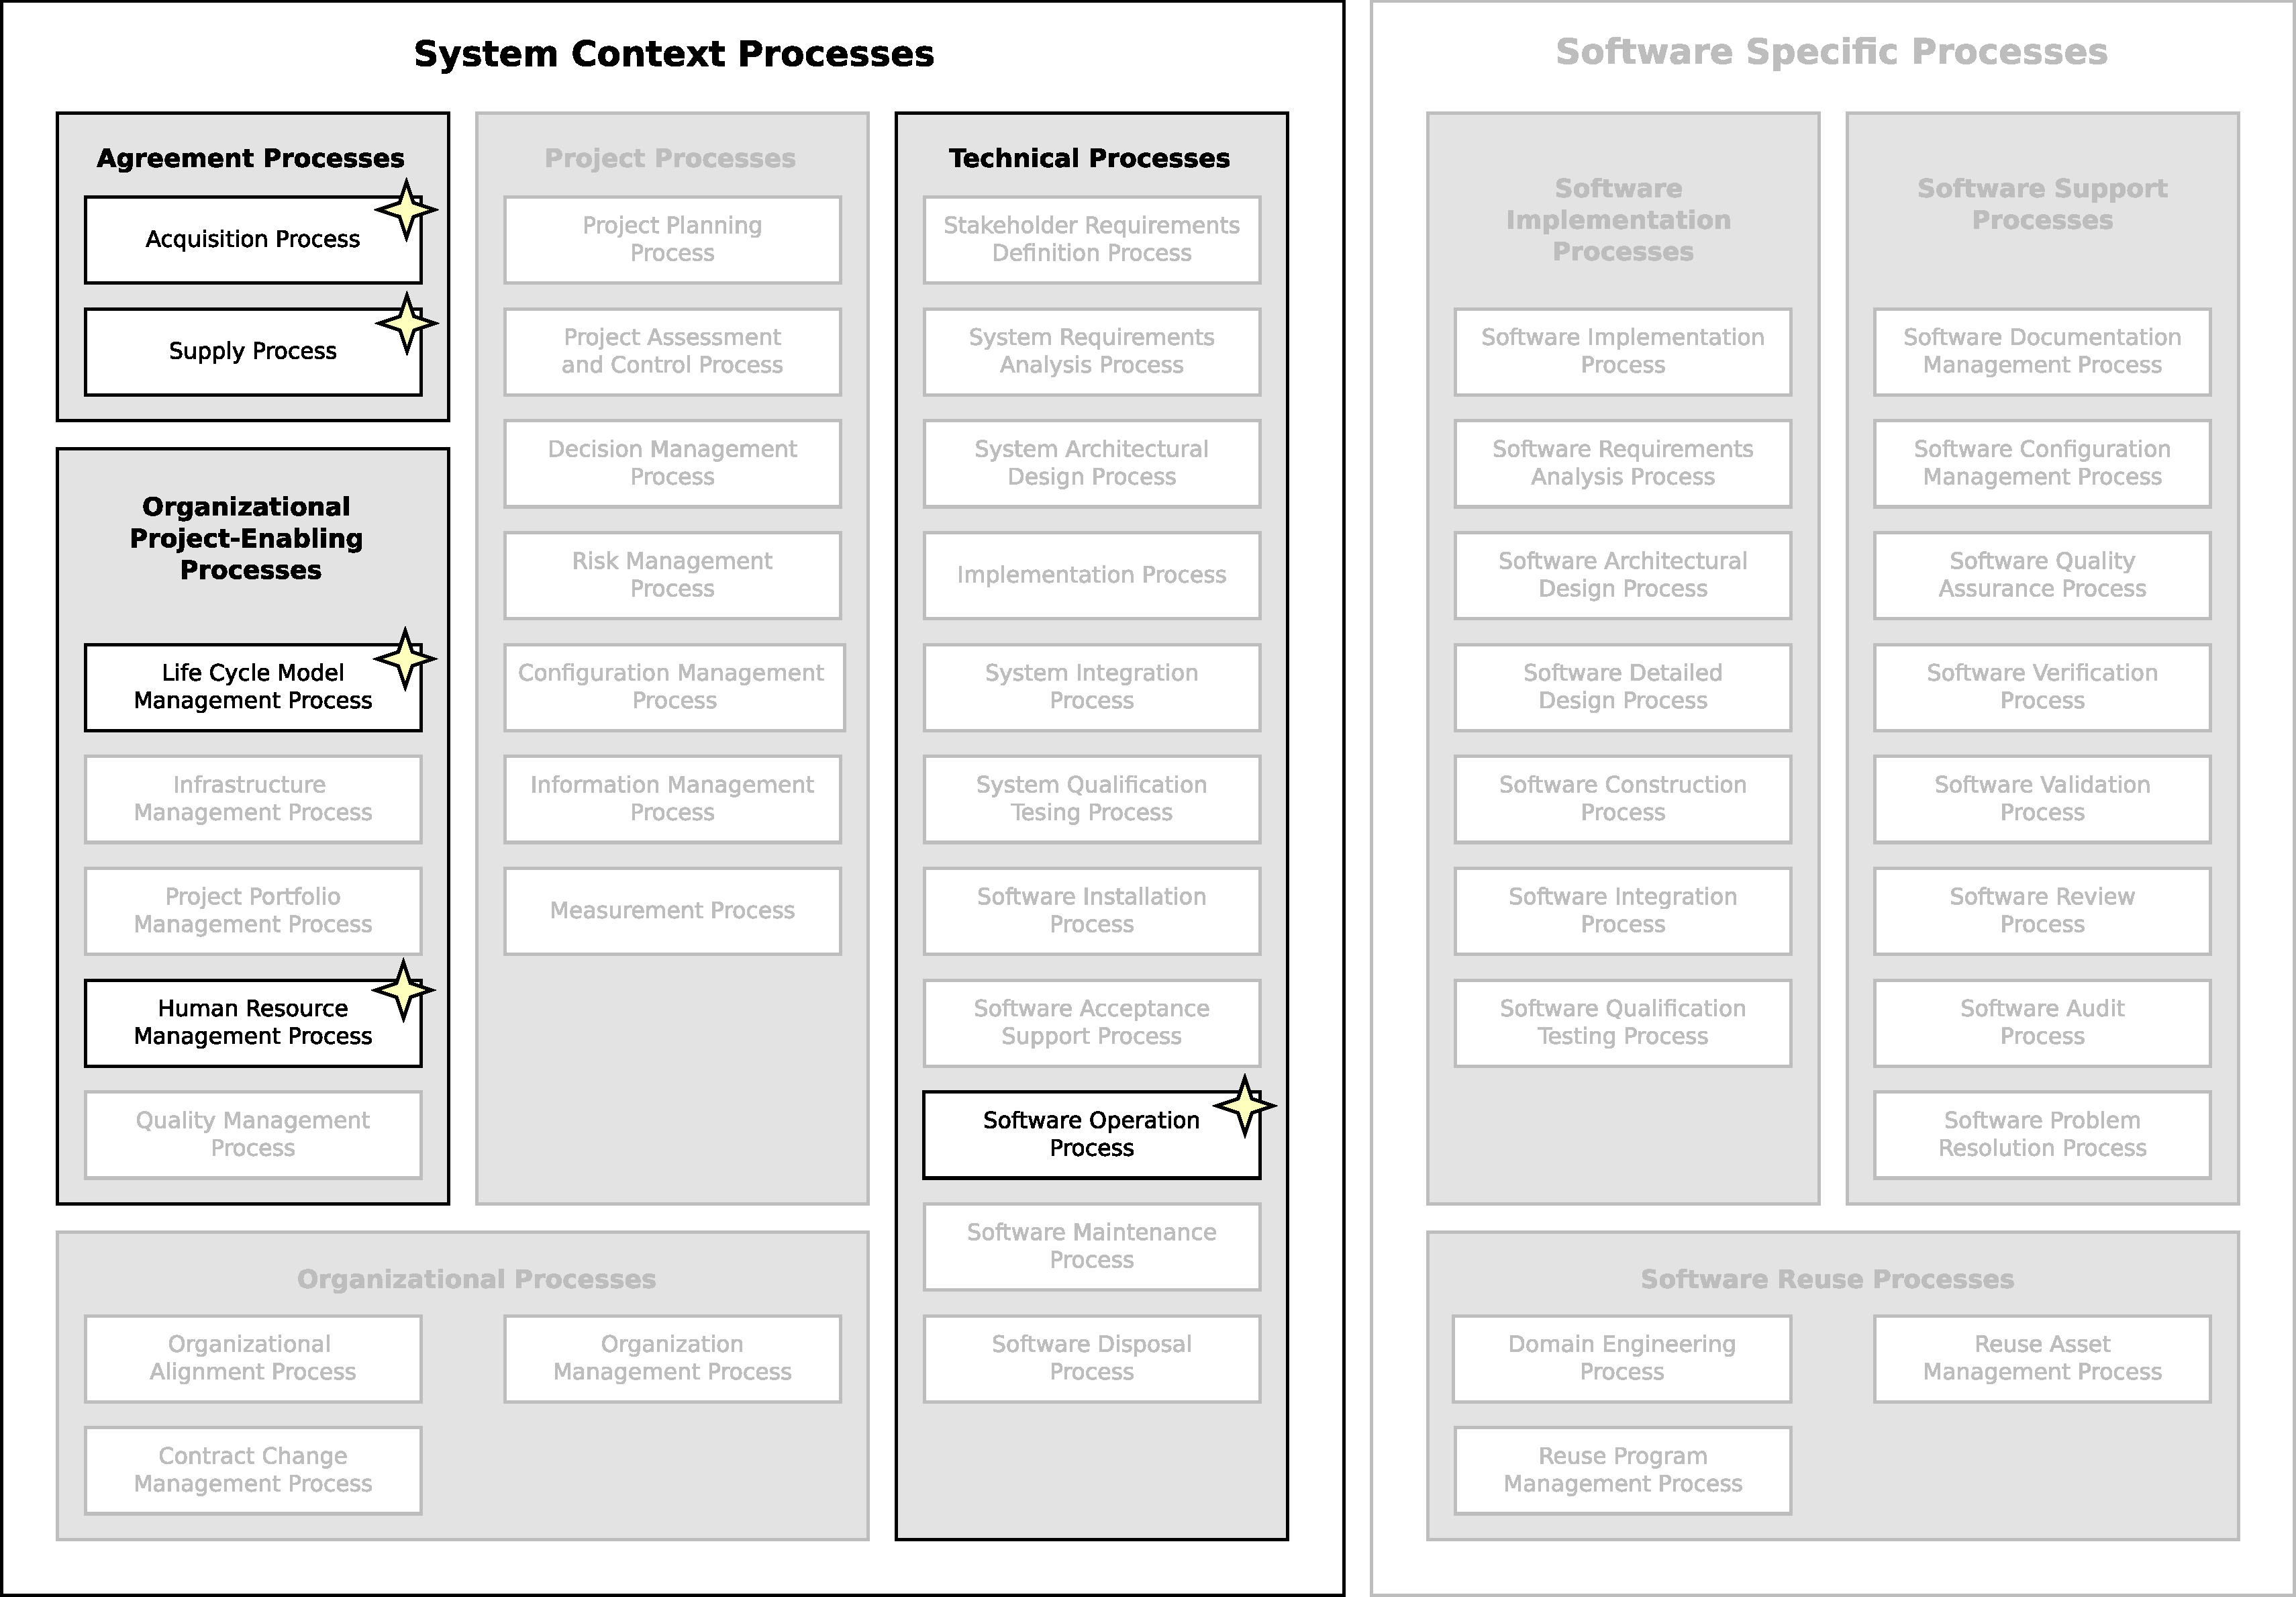
\includegraphics[width=15cm,keepaspectratio]{figures/life-cycle-process-groups-lower-level-processes.pdf}
	\caption{PROCESS REFERENCE MODEL (PRM) LOWER-LEVEL PROCESSES}
	\label{fig:lower_level_processes}
\end{figure}

\begin{adjustwidth}{1em}{0pt}

	Some of the processes defined within this standard may require additional lower-level processes in order to be realized in certain industries or by certain businesses whose activities are directed or more specific than the processes defined in the primary content of the document seemingly allow.

	Only the purpose and outcomes for these processes has been defined, and the necessary activities for the processes, as they relate to those found in the parent-level process, need to be integrated into said process' activities and tasks in order to extend, and not disrupt, the parent-level process' outcomes, activities, and tasks. 

\end{adjustwidth}

	\newpage
	\subsection{ACQUISITION PROCESS LOWER-LEVEL PROCESSES\label{llsubsec:acquisition_processes}}
	\begin{figure}[h]
		\centering
		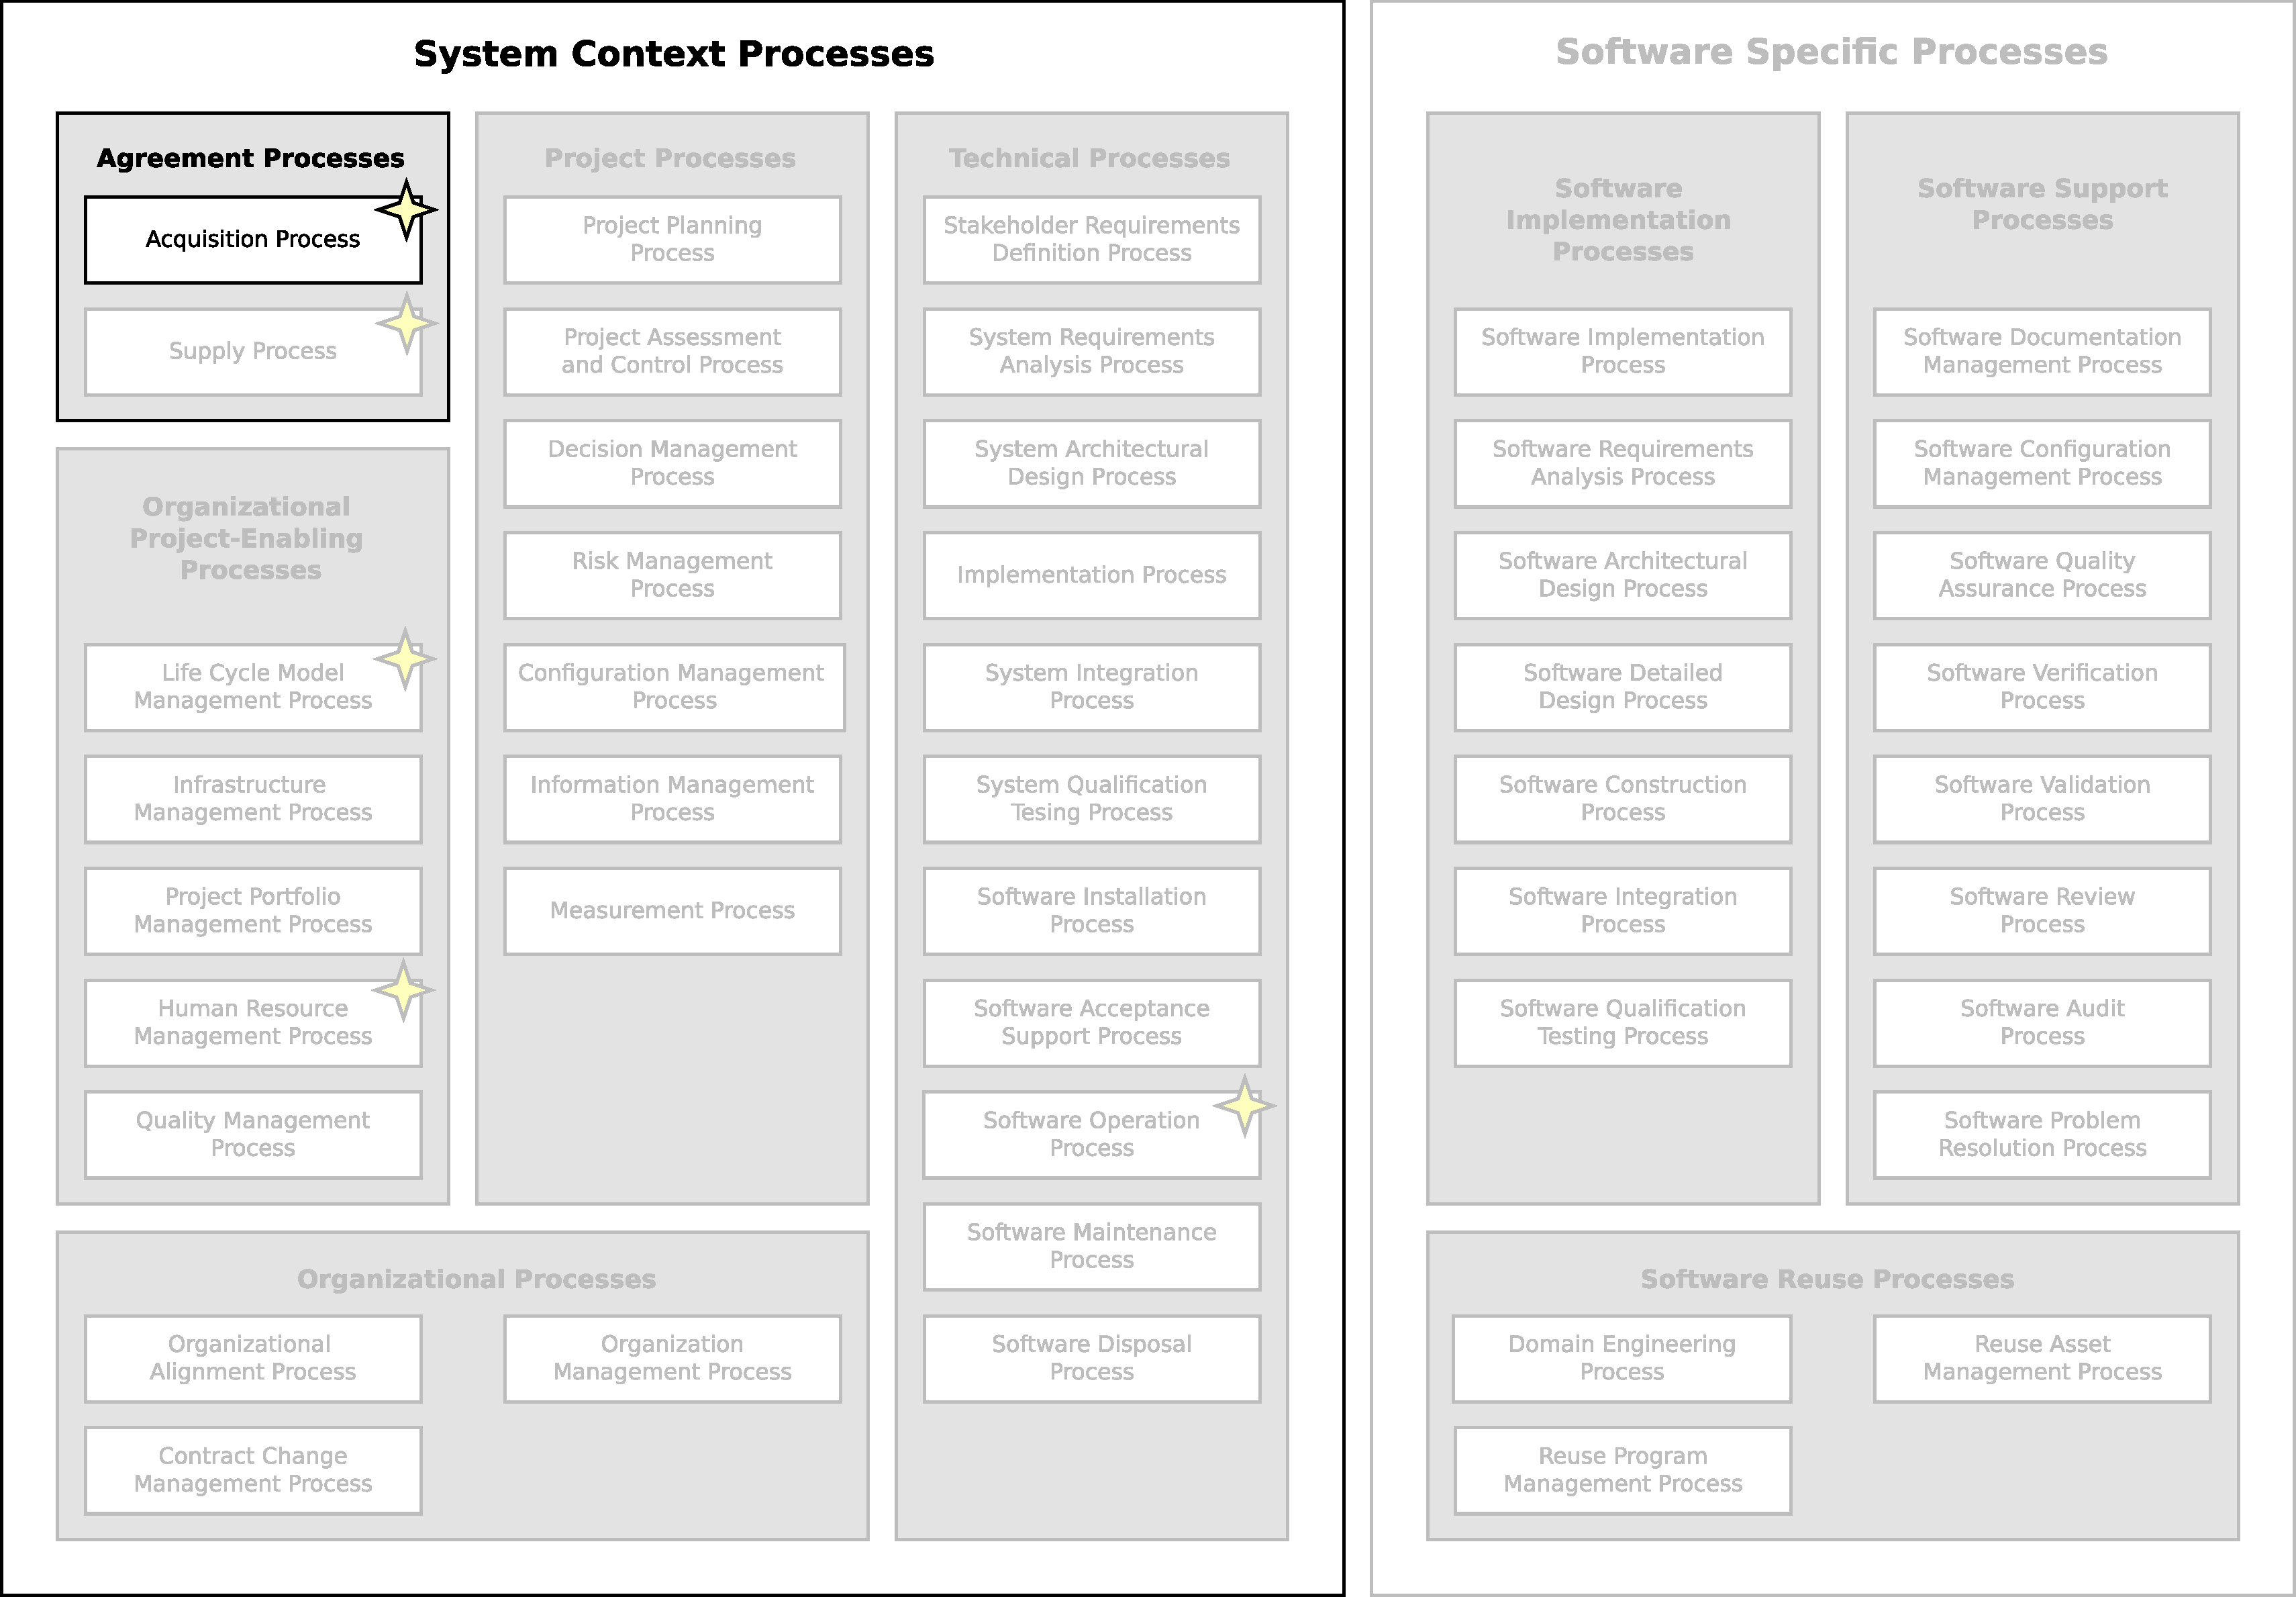
\includegraphics[width=15cm,keepaspectratio]{figures/life-cycle-process-groups-lower-level-acquisition-processes.pdf}
		\caption{Acquisition Process Lower-Level Processes}
		\label{fig:lower_level_acquisition_processes}
	\end{figure}

		\subsubsection{ACQUISITION PREPARATION PROCESS\label{llproc:acquisition_preparation_process}}

			\subsubsubsection{PURPOSE}
			\begin{adjustwidth}{2em}{0pt} 

				The purpose of the \nameref{llproc:acquisition_preparation_process} is to establish the needs and goals of the acquisition and to communicate these with the potential suppliers.

				This process is a lower-level process of the \nameref{proc:acquisition_process}, that replaces the Acquisition Preparation activity.

			\end{adjustwidth}

			\subsubsubsection{OUTCOMES}
			\begin{adjustwidth}{2em}{0pt} 

				\begin{compactitem}

					\item the concept or the need for the acquisition, development, or enhancement is established;

					\item stakeholder requirements are defined;

					\item an acquisition strategy is developed; and

					\item supplier selection criteria are defined.

				\end{compactitem}

			\end{adjustwidth}

		\subsubsection{SUPPLIER SELECTION PROCESS\label{llproc:supplier_selection_process}}

			\subsubsubsection{PURPOSE}
			\begin{adjustwidth}{2em}{0pt} 

				The purpose of the \nameref{llproc:supplier_selection_process} is to choose the organization that is to be responsible for the delivery of the requirements of the project.

				This process is a lower-level process of the \nameref{proc:acquisition_process}, that replaces the Supplier Selection activity.

			\end{adjustwidth}

			\subsubsubsection{OUTCOMES}
			\begin{adjustwidth}{2em}{0pt} 

				\begin{compactitem}

					\item the supplier selection criteria are established and used to evaluate potential suppliers;

					\item the supplier is selected based upon the evaluation of the supplier's proposals, process capabilities, and other factors; and

					\item an agreement is established and negotiated between the acquirer and the supplier.

				\end{compactitem}

			\end{adjustwidth}

		\subsubsection{AGREEMENT MONITORING PROCESS\label{llproc:agreement_monitoring_process}}

			\subsubsubsection{PURPOSE}
			\begin{adjustwidth}{2em}{0pt} 

				The purpose of the \nameref{llproc:agreement_monitoring_process} is to track and assess performance of the supplier against agreed requirements.

				This process is a lower level-process of the \nameref{proc:acquisition_process}. It replaces the Agreement Monitoring activity.

			\end{adjustwidth}

			\subsubsubsection{OUTCOMES}
			\begin{adjustwidth}{2em}{0pt} 

				\begin{compactitem}

					\item joint activities between the acquirer and the supplier are performed as needed;

					\item information on technical progress is exchanged regularly with the supplier;

					\item performance of the supplier is monitored against the agreed requirements; and

					\item agreement changes, if needed, are negotiated between the acquirer and the supplier and documented in the agreement.

				\end{compactitem}

			\end{adjustwidth}

		\subsubsection{ACQUIRER ACCEPTANCE PROCESS\label{llproc:acquirer_acceptance_process}}

			\subsubsubsection{PURPOSE}
			\begin{adjustwidth}{2em}{0pt} 

				The purpose of the \nameref{llproc:acquirer_acceptance_process} is to approve the supplier's deliverable when all acceptance criteria are satisfied.

				This process is a lower-level process of the \nameref{proc:acquisition_process}. It replaces the Acquirer Acceptance activity.

			\end{adjustwidth}

			\subsubsubsection{OUTCOMES}
			\begin{adjustwidth}{2em}{0pt} 

				\begin{compactitem}

					\item the delivered software product and/or service are evaluated with regard to the agreement;

					\item the acquirer's acceptance is based on the agreed acceptance criteria; and

					\item the software product and/or service is accepted by the acquirer.

				\end{compactitem}

			\end{adjustwidth}



	\newpage
	\subsection{SUPPLY PROCESS LOWER-LEVEL PROCESSES\label{llsubsec:supply_processes}}
	\begin{figure}[h]
		\centering
		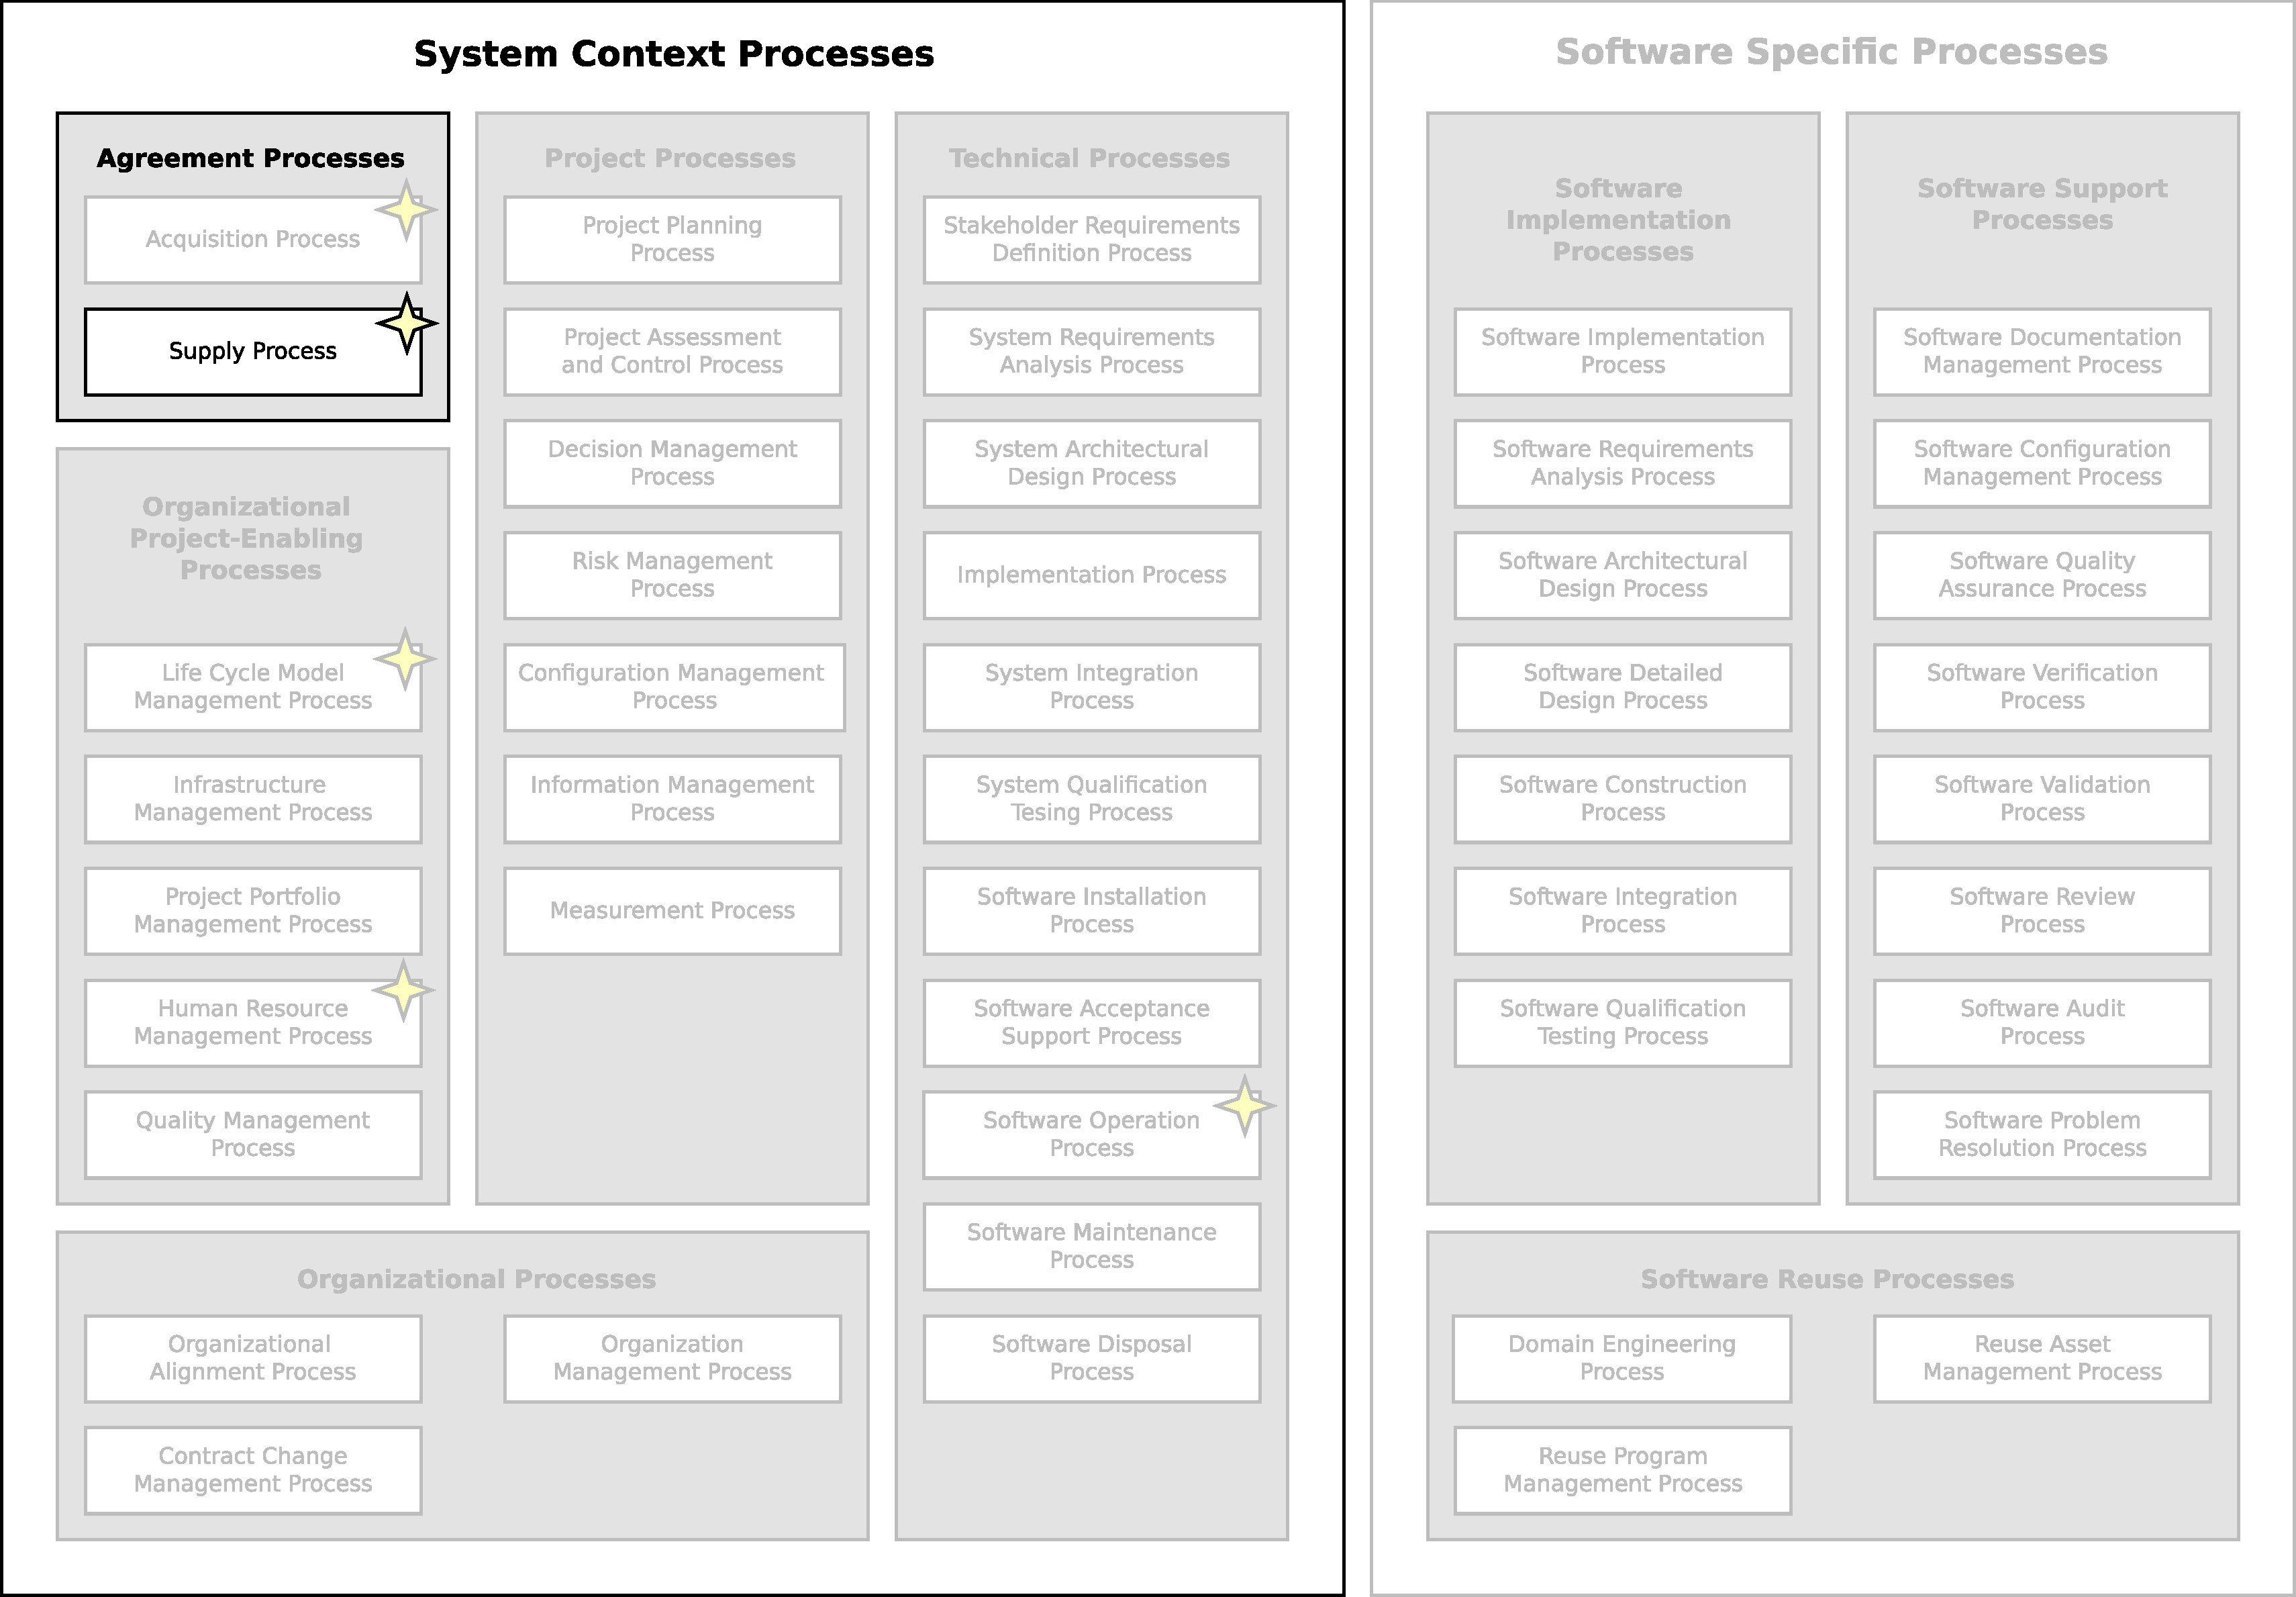
\includegraphics[width=15cm,keepaspectratio]{figures/life-cycle-process-groups-lower-level-supply-processes.pdf}
		\caption{Supply Process Lower-Level Processes}
		\label{fig:lower_level_supply_processes}
	\end{figure}
		
		\subsubsection{SUPPLIER TENDERING PROCESS\label{llproc:supplier_tendering_process}}

			\subsubsubsection{PURPOSE}
			\begin{adjustwidth}{2em}{0pt} 

				The purpose of the \nameref{llproc:supplier_tendering_process} is to establish an interface to respond to acquirer inquiries and requests for proposal, prepare and submit proposals.

				This process is a lower level-process of the \nameref{proc:supply_process}. It replaces the Supplier Tendering activity.

			\end{adjustwidth}

			\subsubsubsection{OUTCOMES}
			\begin{adjustwidth}{2em}{0pt} 

				\begin{compactitem}

					\item a communication interface is established and maintained in order to respond to acquirer inquiries and requests for proposal;

					\item requests for proposal are evaluated according to defined criteria to determine whether or not to submit a proposal;

					\item the need to undertake preliminary surveys or feasibility studies is determined;

					\item suitable resources are identified to perform the proposed work; and

					\item a supplier proposal is prepared and submitted in response to the acquirer request.

				\end{compactitem}

			\end{adjustwidth}

		\subsubsection{CONTRACT AGREEMENT PROCESS\label{llproc:contract_agreement_process}}

			\subsubsubsection{PURPOSE}
			\begin{adjustwidth}{2em}{0pt} 
				
				The purpose of \nameref{llproc:contract_agreement_process} is to negotiate and approve a contract/agreement that clearly and unambiguously specifies the expectations, responsibilities, work products/deliverables and liabilities of both the supplier and the acquirer.

				This process is a lower level-process of the \nameref{proc:supply_process}. It replaces the Contract Agreement activity.

			\end{adjustwidth}

			\subsubsubsection{OUTCOMES}
			\begin{adjustwidth}{2em}{0pt} 

				\begin{compactitem}

					\item a contract/agreement is negotiated, reviewed, approved and awarded to the supplier(s);

					\item mechanisms for monitoring the capability and performance of the supplier(s) and for mitigation of identified risks are reviewed and considered for inclusion in the contract conditions;

					\item proposers/tenderers are notified of the result of proposal/tender selection; and

					\item formal confirmation of agreement is obtained.

				\end{compactitem}

			{\bf Note}: The \nameref{llproc:contract_agreement_process} is used to obtain formal confirmation of assignments that were offered during the \nameref{llproc:supplier_tendering_process}.


			\end{adjustwidth}

		\subsubsection{PRODUCT AND SERVICE DELIVERY AND SUPPORT PROCESS\label{llproc:product_and_service_delivery_and_support_process}}

			\subsubsubsection{PURPOSE}
			\begin{adjustwidth}{2em}{0pt} 

				The purpose of the \nameref{llproc:product_and_service_delivery_and_support_process} is to provide the specified product or service to the acquirer with support appropriate to achieve confidence that the requirements have been met.

				This process is a lower-level process of the \nameref{proc:supply_process}. It replaces the Product/Service Delivery and Support activity.

			\end{adjustwidth}

			\subsubsubsection{OUTCOMES}
			\begin{adjustwidth}{2em}{0pt} 

				\begin{compactitem}

					\item the contents of the product release are determined;

					\item the release is assembled from configured items;

					\item the release documentation is defined and produced;

					\item the release delivery mechanism and media are determined;

					\item release approval is effected against defined criteria;

					\item the product release is made available to the acquirer;

					\item confirmation of release is obtained;

					\item the product is completed and delivered to the acquirer;

					\item acquirer acceptance tests and reviews are supported;

					\item the product is put into operation in the customers’ environment; and

					\item problems detected during acceptance are identified and communicated to those responsible for resolution.

				\end{compactitem}

			{\bf Note}: Incremental delivery would be in completed increments.

			\end{adjustwidth}


	\newpage
	\subsection{LIFE CYCLE MODEL MANAGEMENT PROCESS LOWER-LEVEL PROCESSES\label{llsubsec:life_cycle_model_management_processes}}
	\begin{figure}[h]
		\centering
		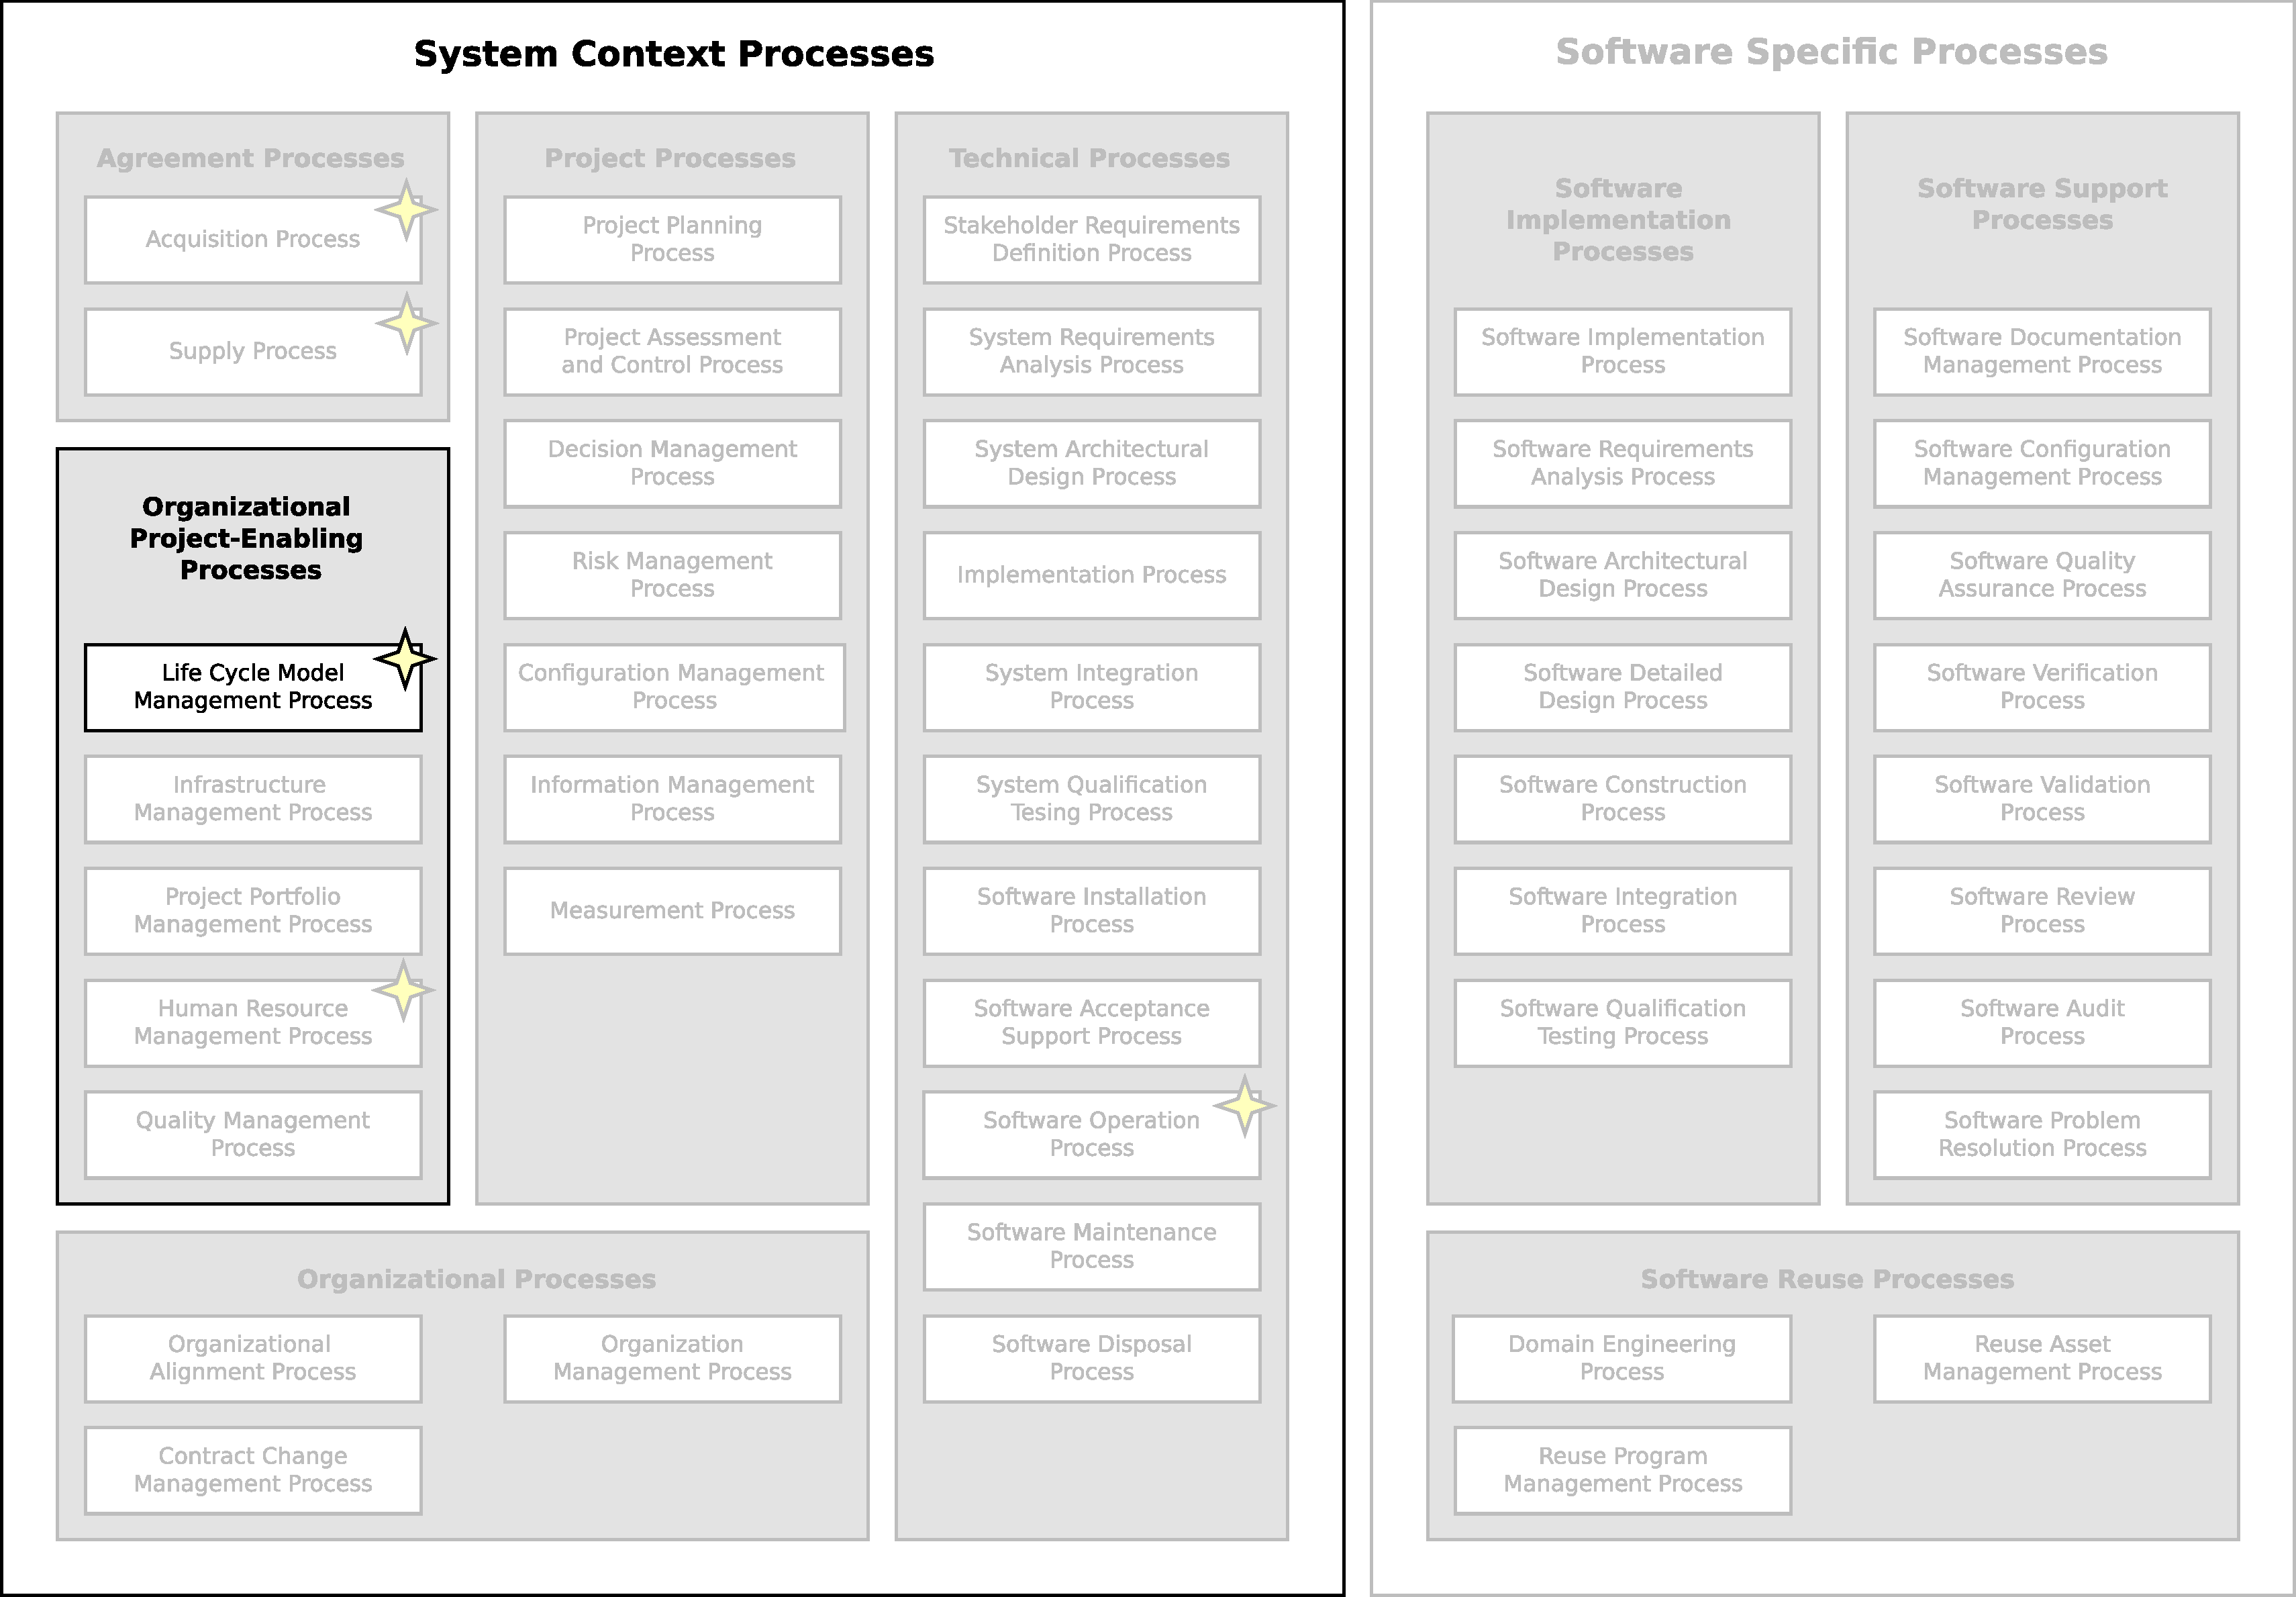
\includegraphics[width=15cm,keepaspectratio]{figures/life-cycle-process-groups-lower-level-life-cycle-model-management-processes.pdf}
		\caption{Life Cycle Model Management Process Lower-Level Processes}
		\label{fig:lower_level_life_cycle_model_management_processes}
	\end{figure}

		\subsubsection{PROCESS ESTABLISHMENT PROCESS\label{llproc:process_establishment_process}}

			\subsubsubsection{PURPOSE}
			\begin{adjustwidth}{2em}{0pt} 

				The purpose of the \nameref{llproc:process_establishment_process} is to establish a suite of organizational processes for all life cycle processes as they apply to its business activities.

				This process is a lower-level process of the \nameref{proc:life_cycle_model_management_process}. It replaces the Process Establishment activity.

			\end{adjustwidth}

			\subsubsubsection{OUTCOMES}
			\begin{adjustwidth}{2em}{0pt} 

				\begin{compactitem}

					\item a defined and maintained standard set of processes are established, along with an indication of each process's applicability;

					\item the detailed tasks, activities and associated work products of the standard process are identified, together with expected performance characteristics;

					\item a strategy for tailoring the standard process for the product or service is developed in accordance with the needs of the project; and

					\item information and data related to the use of the standard process for specific projects exist and are maintained.

				\end{compactitem}

			\end{adjustwidth}

		\subsubsection{PROCESS ASSESSMENT PROCESS\label{llproc:process_assessment_process}}

			\subsubsubsection{PURPOSE}
			\begin{adjustwidth}{2em}{0pt} 
				
				The purpose of the \nameref{llproc:process_assessment_process} is to determine the extent to which the organization's standard processes contribute to the achievement of its business goals and to help the organization focus on the need for continuous process improvement.

				This process is a lower-level process of the \nameref{proc:life_cycle_model_management_process}, that replaces its Process Assessment activity.

			\end{adjustwidth}

			\subsubsubsection{OUTCOMES}
			\begin{adjustwidth}{2em}{0pt} 

				\begin{compactitem}

					\item information and data related to the use of the standard process for specific projects exists and is maintained;

					\item the relative strengths and weaknesses of the organization's standard processes are understood; and

					\item accurate and accessible assessment records are kept and maintained.

				\end{compactitem}

			\end{adjustwidth}

		\subsubsection{PROCESS IMPROVEMENT PROCESS\label{llproc:process_improvement_process}}

			\subsubsubsection{PURPOSE}
			\begin{adjustwidth}{2em}{0pt} 
				
				The purpose of the \nameref{llproc:process_improvement_process} is to continually improve the organization's effectiveness and efficiency through the processes used and maintained and aligned with the business need.

				This process is a lower-level process of the \nameref{proc:life_cycle_model_management_process}, that replaces its Process Improvement activity.

			\end{adjustwidth}

			\subsubsubsection{OUTCOMES}
			\begin{adjustwidth}{2em}{0pt} 

				\begin{compactitem}

					\item commitment is established to provide resources to sustain improvement actions;

					\item issues arising from the organization's internal/external environment are identified as improvement opportunities and justified as reasons for change;

					\item analysis of the current status of the existing process is performed, focusing on those processes from which improvement stimuli arise;
					
					\item improvement goals are identified and prioritized, and consequent changes to the process are defined and implemented; 					

					\item the effects of process implementation are monitored and confirmed against the defined improvement goals;
					
					\item knowledge gained from the improvements is communicated within the organization; and

					\item the improvements made are evaluated and consideration given for using solutions elsewhere within the organization.

				\end{compactitem}


				{\bf Note 1}: Information sources providing input for change may include: process assessment results, audits, customer's satisfaction reports, organizational effectiveness/efficiency, cost of quality.

				{\bf Note 2}: The current status of processes may be determined by process assessment.


			\end{adjustwidth}


	\newpage
	\subsection{HUMAN RESOURCE MANAGEMENT PROCESS LOWER-LEVEL PROCESSES\label{llsubsec:human_resource_management_processes}}
	\begin{figure}[h]
		\centering
		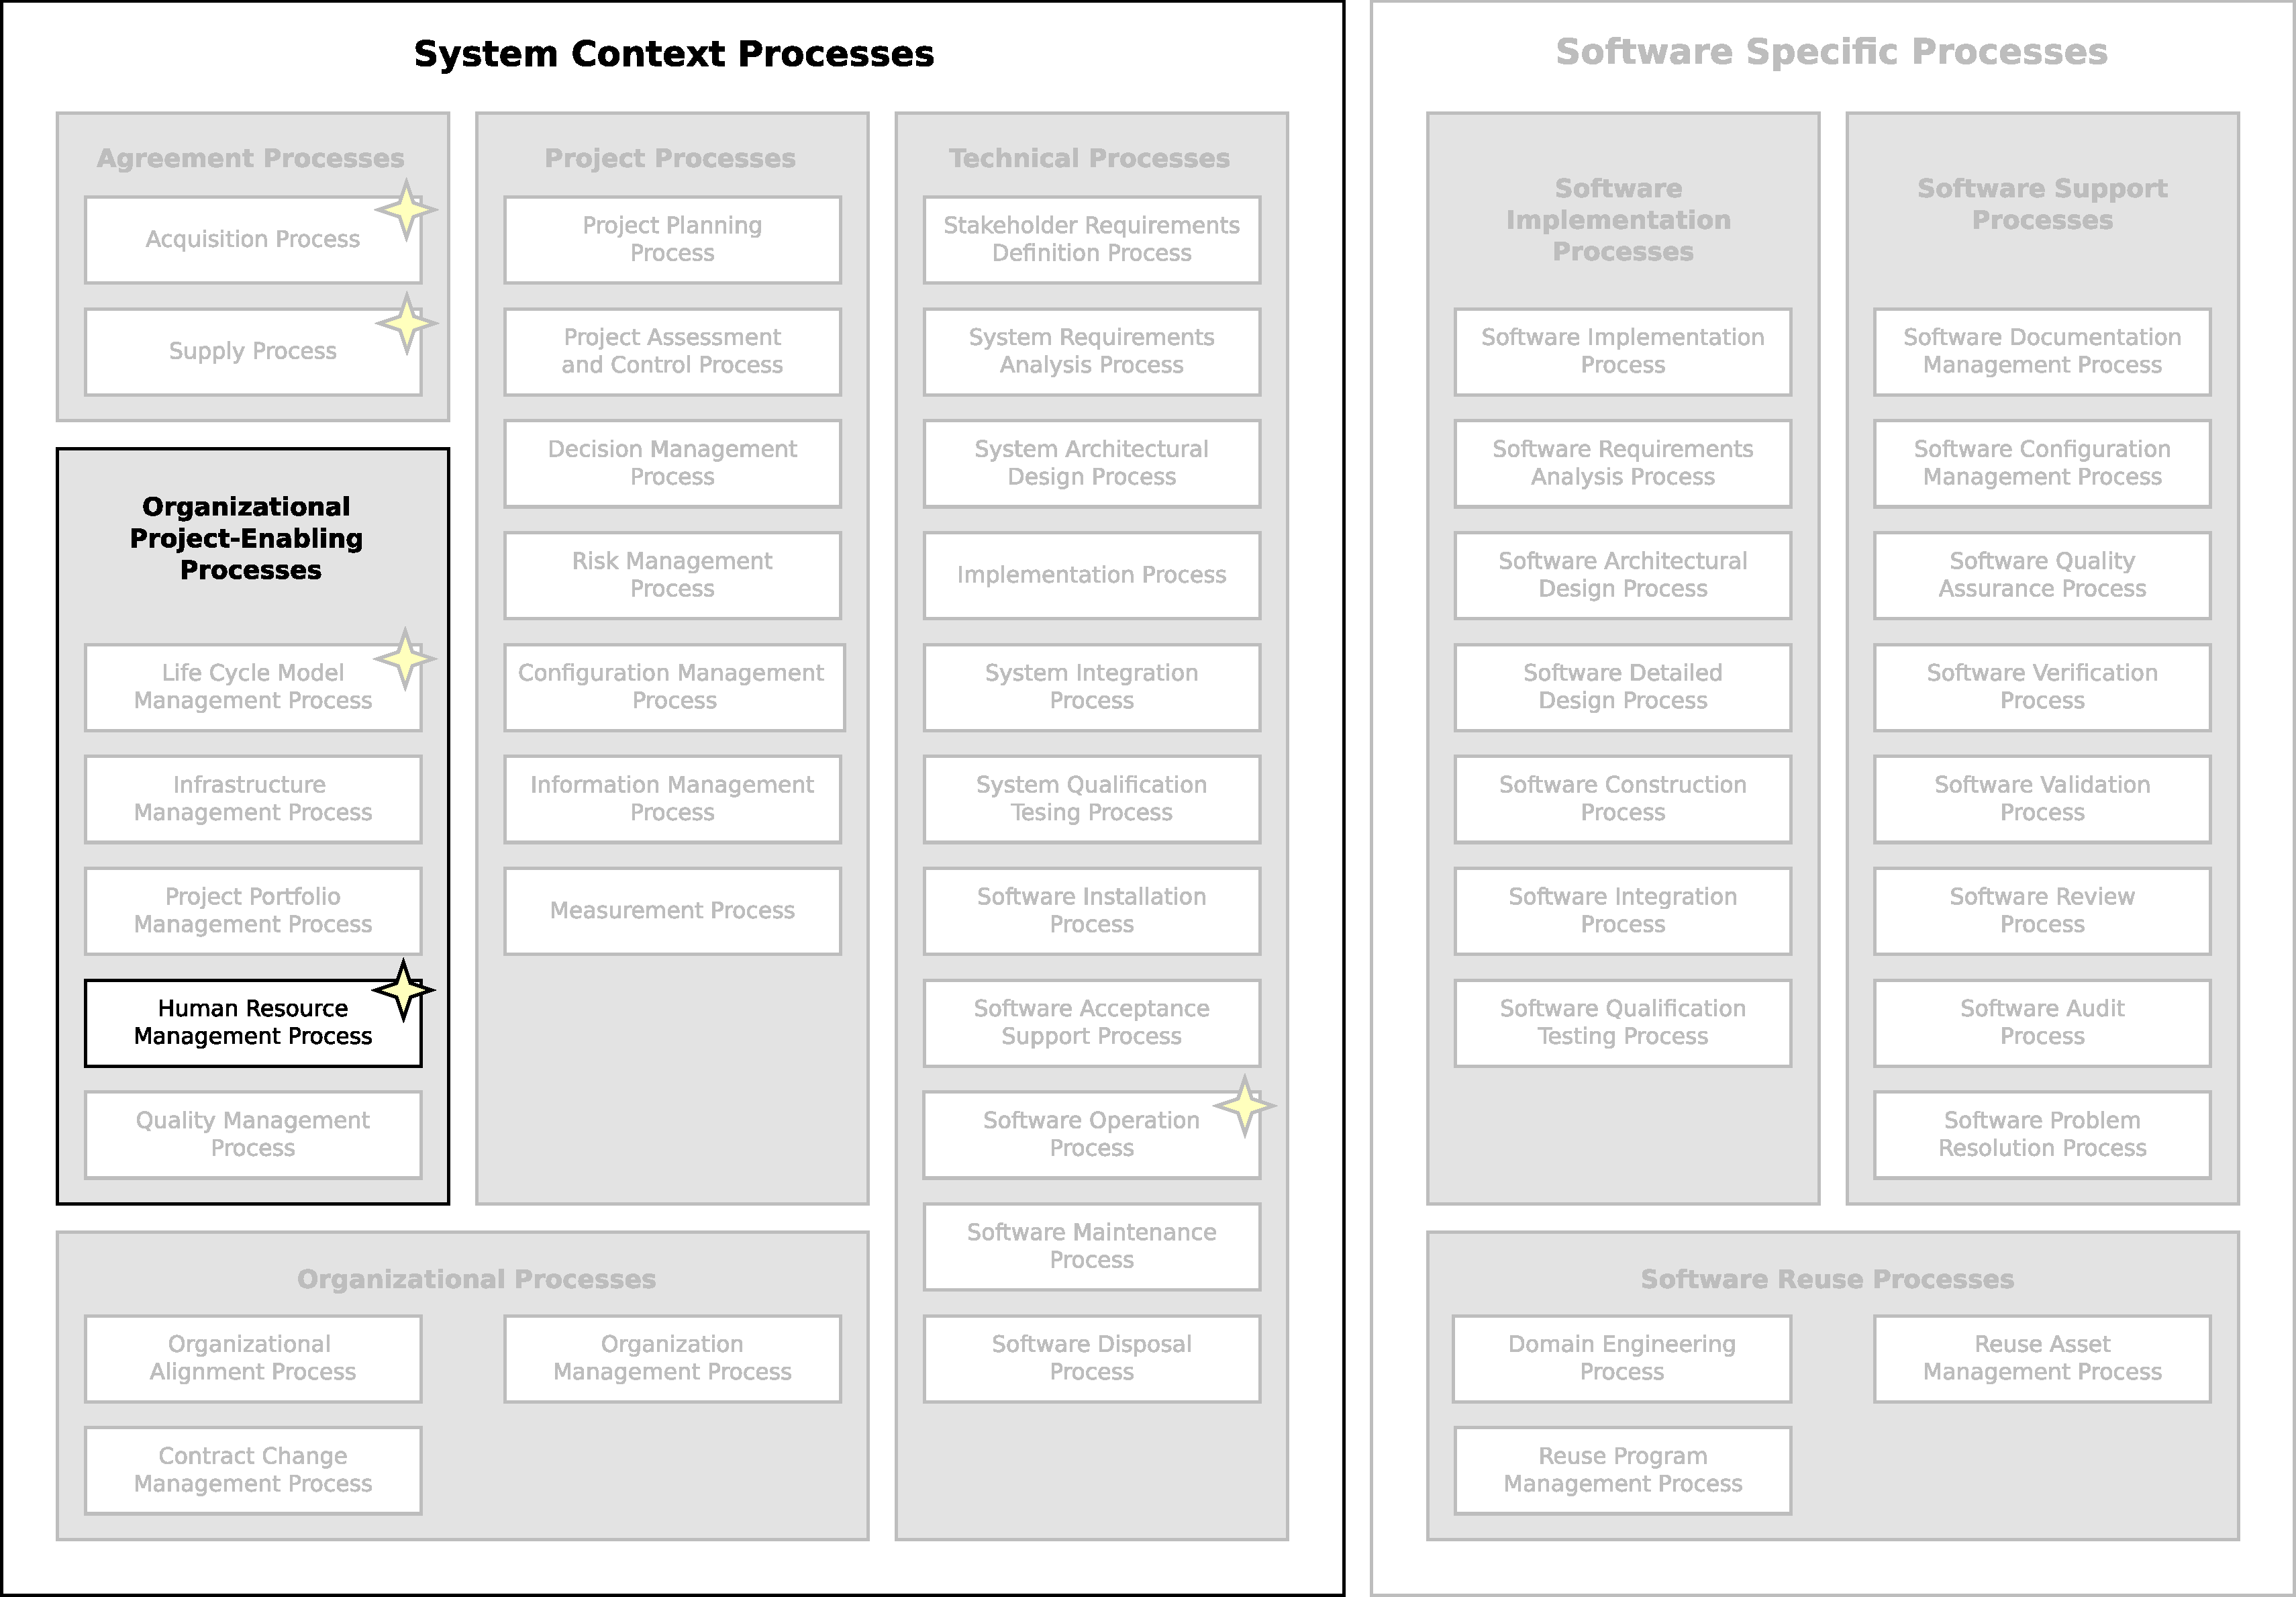
\includegraphics[width=15cm,keepaspectratio]{figures/life-cycle-process-groups-lower-level-human-resource-management-processes.pdf}
		\caption{Human Resource Management Lower-Level Processes}
		\label{fig:lower_level_human_resource_management_processes}
	\end{figure}

		\subsubsection{SKILL DEVELOPMENT PROCESS\label{llproc:skill_development_process}}

			\subsubsubsection{PURPOSE}
			\begin{adjustwidth}{2em}{0pt} 

				The purpose of the \nameref{llproc:skill_development_process} is to provide the organization and project with individuals who possess the needed skills and knowledge to perform their roles effectively.

				This process is a lower-level process of the \nameref{proc:human_resource_management_process}. It replaces the Skill Development activity.

			\end{adjustwidth}

			\subsubsubsection{OUTCOMES}
			\begin{adjustwidth}{2em}{0pt} 

				\begin{compactitem}

					\item training is developed or acquired to address the organization and project training needs; and

					\item training is conducted to ensure that all individuals have the skills required to perform their assignments, using mechanisms such as training strategies and materials.

				\end{compactitem}

			\end{adjustwidth}

		\subsubsection{SKILL ACQUISITION PROCESS\label{llproc:skill_acquisition_process}}

			\subsubsubsection{PURPOSE}
			\begin{adjustwidth}{2em}{0pt} 

				The purpose of the \nameref{llproc:skill_acquisition_process} is to provide the organization and projects with individuals who possess skills and knowledge to perform their roles effectively and to work together as a cohesive group.

				This process is a lower-level process of the \nameref{proc:human_resource_management_process}. It replaces the Skill Acquisition and Provision activity.

			\end{adjustwidth}

			\subsubsubsection{OUTCOMES}
			\begin{adjustwidth}{2em}{0pt} 

				\begin{compactitem}

					\item individuals with the required skills and competencies are identified and recruited;

					\item effective interaction between individuals and groups are supported;

					\item the work force have the skills to share information and co-ordinate their activities efficiently; and

					\item objective criteria are defined against which group and individual performance is monitored to provide performance feedback and to enhance performance.

				\end{compactitem}

			\end{adjustwidth}

		\subsubsection{KNOWLEDGE MANAGEMENT PROCESS\label{llproc:knowledge_management_process}}

			\subsubsubsection{PURPOSE}
			\begin{adjustwidth}{2em}{0pt} 

				The purpose of the \nameref{llproc:knowledge_management_process} is to ensure that individual knowledge, information and skills are collected, shared, reused and improved throughout the organization.

				This process is a lower-level process of the \nameref{proc:human_resource_management_process}. It replaces the Knowledge Management activity.

			\end{adjustwidth}

			\subsubsubsection{OUTCOMES}
			\begin{adjustwidth}{2em}{0pt} 

				\begin{compactitem}

					\item infrastructure is established and maintained for sharing common and domain information across the organization;

					\item knowledge is readily available and shared throughout the organization; and

					\item the organization selects an appropriate knowledge management strategy.

				\end{compactitem}

			\end{adjustwidth}


	\newpage
	\subsection{SOFTWARE OPERATION PROCESS LOWER-LEVEL PROCESSES\label{llsubsec:software_operation_processes}}
	\begin{figure}[h]
		\centering
		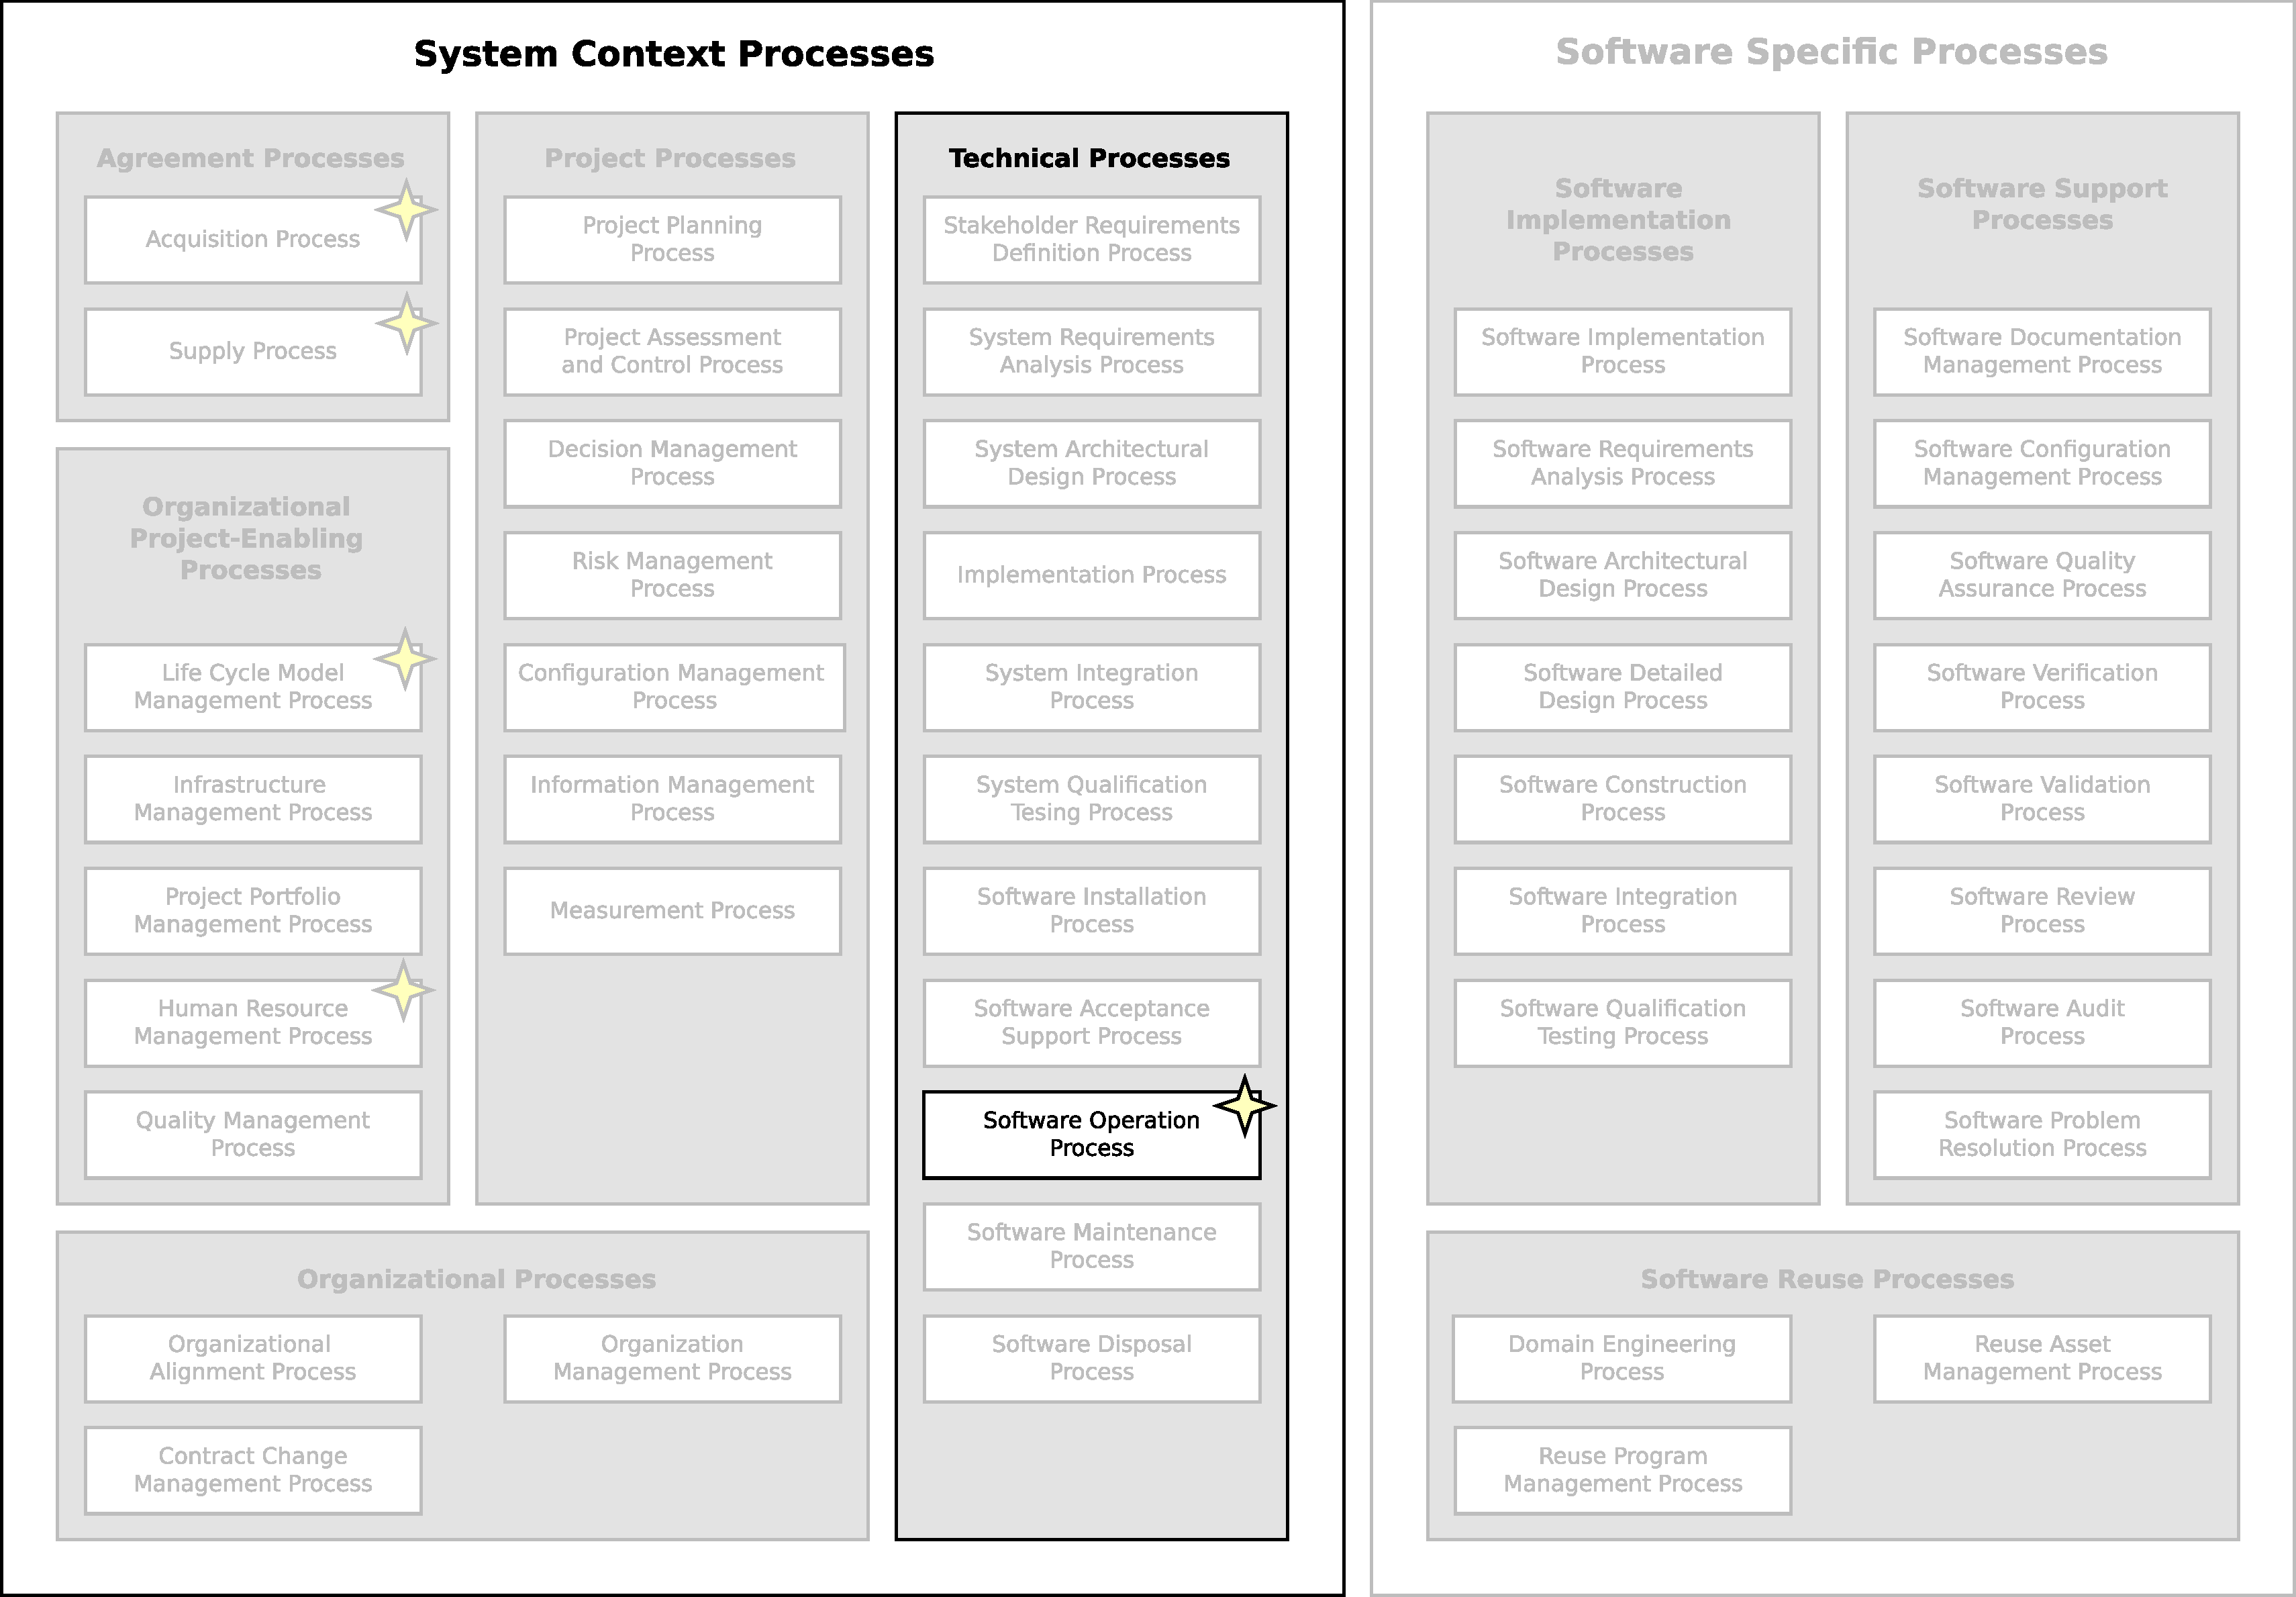
\includegraphics[width=15cm,keepaspectratio]{figures/life-cycle-process-groups-lower-level-software-operation-processes.pdf}
		\caption{Software Operation Process Lower-Level Processes}
		\label{fig:lower_level_software_operation_processes}
	\end{figure}

		\subsubsection{OPERATIONAL USE PROCESS\label{llproc:operational_use_process}}

			\subsubsubsection{PURPOSE}
			\begin{adjustwidth}{2em}{0pt} 

				The purpose of the \nameref{llproc:operational_use_process} is to ensure the correct and efficient operation of the product for the duration of its intended usage and in its installed environment.

				This process is a lower-level process of the \nameref{proc:software_operation_process}. It replaces the Operational Use activity.

			\end{adjustwidth}

			\subsubsubsection{OUTCOMES}
			\begin{adjustwidth}{2em}{0pt} 

				\begin{compactitem}

					\item operational risks for the product introduction and operation are identified and monitored;

					\item the product is operated in its intended environment according to requirements; and

					\item criteria for the operational use are developed that demonstrates compliance with the agreed requirements.

				\end{compactitem}

			\end{adjustwidth}

		\subsubsection{CUSTOMER SUPPORT PROCESS\label{llproc:customer_support_process}}

			\subsubsubsection{PURPOSE}
			\begin{adjustwidth}{2em}{0pt} 

				The purpose of the \nameref{llproc:customer_support_process} is to establish and maintain an acceptable level of service through assistance and consultation to the customer to support effective use of the product.

				This process is a lower-level process of the \nameref{proc:software_operation_process}. It replaces the Customer Support activity.

			\end{adjustwidth}

			\subsubsubsection{OUTCOMES}
			\begin{adjustwidth}{2em}{0pt} 

				\begin{compactitem}

					\item service needs for customer support are identified and monitored on an ongoing basis;

					\item customer satisfaction with both the support services being provided and the product itself is evaluated on an ongoing basis;

					\item operational support is provided by handling customer inquiries and requests and resolving operational problems; and

					\item customer support needs are met through delivery of appropriate services.

				\end{compactitem}

			\end{adjustwidth}


	\newpage
	
\section{PROCESS VIEWS\label{llsec:process_views}}
\begin{adjustwidth}{0em}{0pt}

	There are instances where those representing a particular engineering interest would like to see gathered in a single place the set of process activities that directly and succinctly address their concern. For such interests, a process view can be developed to organize processes, activities, and tasks selected from this and other standards to provide a focus to their particular concern in a manner that cuts across all or parts of the life cycle. This appendix provides a process viewpoint that may be used to define process views in these instances.

\end{adjustwidth}
		

	\subsection{THE PROCESS VIEW CONCEPT\label{subsec:process_view_concept}}
	\begin{adjustwidth}{0.5em}{0pt}

		There may be cases where a unified focus is needed for activities and tasks that are selected from disparate processes to provide visibility to a significant concept or thread that cuts across the processes employed across the life cycle. It is useful to advise users of the standards how to identify and define these activities for their use, even though they cannot locate a single process that addresses their specific concern.

		For this purpose, the concept of a process view has been formulated. Like a process, the description of a process view includes a statement of purpose and outcomes. Unlike a process, the description of a process view does not include activities and tasks. Instead, the description includes guidance explaining how the outcomes can be achieved by employing the activities and tasks of the various processes in this standard. Process views can be constructed using the process viewpoint template found in the \nameref{subsubsec:process_viewpoint} sub-section below.

	\end{adjustwidth}


	\subsection{PROCESS VIEWPOINT \label{subsubsec:process_viewpoint}}
	\begin{adjustwidth}{0.5em}{0pt}

		A process view conforms to a process viewpoint. The process viewpoint provided here can be used to create process views. E.4 contains an example of applying this viewpoint.
		
		The Process Viewpoint is defined by:

		\begin{compactitem}
			
			\item its stakeholders: users of the standard;

			\item the concerns it frames: the processes needed to reflect a particular engineering interest;

			\item the contents of resulting process views should include:

			\item process view name;

			\item process view purpose;

			\item process view outcomes; and

			\item identification and description of the processes, activities and tasks which implement the process view, and references to the sources for these processes, activities and tasks in other standards.

		\end{compactitem}

	\end{adjustwidth}


	\subsection{EXAMPLE: PROCESS VIEW FOR USABILITY \label{subsubsec:example_process_view_for_usability}}
	\begin{adjustwidth}{0.5em}{0pt}

		This section provides an example of applying the process viewpoint to yield a process view for Usability, intended to illustrate how a project might assemble processes, activities and tasks of this standard to provide focused attention to the achievement of a usable product.

		This example treats the cluster of interests, generally called Usability, User centered design or Human-centered design that enables optimizing support and training, increased productivity and quality of work, improved human working conditions and reducing the chance of user rejection of the system.

		{\bf Name}: {\it Usability Process View}

	\end{adjustwidth}

		\subsubsubsection{PURPOSE}
		\begin{adjustwidth}{2em}{0pt}

			The purpose of the Usability Process View is to ensure the consideration of the interests and needs of the stakeholders in order to enable optimizing support and training, increased productivity and quality of work, improved human working conditions and reducing the chance of user rejection of the system.
			
			As a result of successful implementation of the {\it Usability Process View}:

			\begin{compactitem}

				\item the system meets the needs of users and takes account of their human capabilities and skill limitations;

				\item human factors and ergonomics knowledge and techniques are incorporated in systems design;

				\item human-centered design activities are identified and performed;

				\item system design will address possible adverse effects of use on human health, safety and performance; and

				\item systems will have enhanced user effectiveness, efficiency and satisfaction.

			\end{compactitem}

			{\bf Note}: Although involvement of users is a principle of human centered design, the outcomes permit the possibility that the desired characteristics cannot be directly measured but instead might be argued and inferred based on other product or process characteristics that can be measured.

		\end{adjustwidth}


		\subsubsubsection{PROCESSES, ACTIVITIES, TASKS}
		\begin{adjustwidth}{2em}{0pt}

			This process view can be implemented using the following processes, activities, and tasks from this standard.

			\begin{compactenum}

				\item The \nameref{proc:project_portfolio_management_process}, in particular the Process Initiation activity, provides for the establishment and maintenance of a focus on user issues in the parts of the organization that deal with markets, concept, development and support; championing of a human-centered approach.

				\item The \nameref{proc:infrastructure_management_process} provides a specification of how human-centered design activities fit into the whole systems life cycle process and the organization.

				\item The \nameref{proc:project_planning_process} provides for: selection of human centered methods and techniques, planning the involvement of users and other stakeholders, planning of human-centered design activities.

				\item The \nameref{proc:project_assessment_and_control_process} provides for monitoring the extent of achievement of the requirements and communicating the results to stakeholders and managers, ensuring a human centered approach in the design team. 

				\item The \nameref{proc:stakeholder_requirements_definition_process} provides for the identification and documentation of the context of use and the interaction between users and the system, taking into account human capabilities and skills limitations and the specification of health, safety, security, environment, training, support and other stakeholder requirements and functions that address possible adverse effects of use of the system on human health and safety.

				\item The \nameref{proc:system_requirements_analysis_process} provides for the specification and evaluation of the context of use and the usability and human centered design requirements.

				\item The \nameref{proc:system_architectural_design_process} provides for the incorporation of design criteria to address the targets for usability and the ergonomic requirements.

				\item The \nameref{proc:system_integration_process} provides for planning the integration, including the considerations for user training and the assurance that the achievement of targets for usability and accordance with ergonomic requirements are verified and recorded.

				\item The \nameref{proc:information_management_process}, in its entirety, provides for the specification, development and maintenance of artifacts for documenting and communicating the extent of achievement. 

				\item The \nameref{proc:measurement_process}, in its entirety, provides for defining an approach that relates measures to desired characteristics. 

				\item \nameref{proc:software_requirements_analysis_process} provides for the specification of the usability and software ergonomics requirements.

				\item The \nameref{proc:software_operation_process} provides for use of the system. Assuring that the usability requirements are appropriately achieved involves monitoring the operation of the system. 

				\item The \nameref{proc:software_maintenance_process} sustains the capabilities of the system, including its usability properties and can be used in its entirety.

			\end{compactenum}

		\end{adjustwidth}

	\newpage
	\section{RELATIONSHIPS BETWEEN STANDARDS}
\begin{adjustwidth}{0.5em}{0pt}

	The purpose of this informative appendix is to describe relationships to other IEEE standards. The itemized breakdown below lists the processes of this standard, this document specifically. For many of those processes, the list suggests IEEE standards that may be helpful in implementing or executing the process. In each case, a note describes the nature of the relationship. 

	\begin{compactitem}
		
		\item \nameref{subsec:agreement_processes}
		\begin{compactitem}
			
			\item \nameref{proc:acquisition_process}: IEEE Std. 1062, recommendation of useful practices that can be selected and applied during software acquisition.

		\end{compactitem}


		\item \nameref{subsec:organizational_project_enabling_processes}
		\begin{compactitem}
			
			\item \nameref{proc:life_cycle_model_management_process}: IEEE Std. 1074, standard describes an approach for the definition of software life cycle processes.

			\item \nameref{proc:infrastructure_management_process}: IEEE Std. 1175 and 1462, describe the integration of CASE tools into productive software engineering environments, and guidelines for the evaluation and selection of CASE tools, respectively. 

			\item \nameref{proc:quality_management_process}: ISO 90003, standard provides guidance for organizations in the application of ISO 9001:2000 to software. 

		\end{compactitem}


		\item \nameref{subsec:project_processes}
		\begin{compactitem}
			
			\item \nameref{proc:project_planning_process}: IEEE Std. 1058 and 1228, describes the format and content of a software project management plan, and the content of a plan for the software aspects of development, procurement, maintenance, and retirement of a safety-critical system, respectively. 

			\item \nameref{proc:risk_management_process}: IEEE Std. 1540, provides a process for the management of software risk.  

			\item \nameref{proc:measurement_process}: IEEE Std. 982.1, 1045, 1061, and 14143.1, provides a set of measures for forecasting and evaluating the reliability of a software product, a consistent terminology for software productivity measures, a methodology for establishing quality requirements, and the fundamental concepts of a class of measures collectively known as functional size, respectively. 

		\end{compactitem}


		\item \nameref{subsec:technical_processes}
		\begin{compactitem}
			
			\item \nameref{proc:stakeholder_requirements_definition_process}: IEEE Std. 1362, provides guidance on the format and content of a Concept of Operations document, describing characteristics of a proposed system from the user's viewpoint.

			\item \nameref{proc:system_requirements_analysis_process}: IEEE Std. 1233, provides guidance on the development of a system requirements specification and the characteristics and qualities of requirements.

			\item \nameref{proc:system_architectural_design_process}, IEEE Std. 1471, recommends a conceptual framework and content for the architectural description of software-intensive systems.

			\item \nameref{proc:software_maintenance_process}: ISO/IEC 14764, provides guidance on implementing the software maintenance process. 

		\end{compactitem}


		\item \nameref{subsec:software_implementation_processes}
		\begin{compactitem}

			\item \nameref{proc:software_requirements_analysis_process}: IEEE Std. 830, recommends the content and characteristic of a software requirements specification.

			\item \nameref{proc:software_architectural_design_process}: IEEE Std. 1471, recommends a conceptual framework and content for the architectural description of software-intensive systems. 

			\item \nameref{proc:software_detailed_design_process}: IEEE Std. 1016, recommends content and organization of a software design description.

			\item \nameref{proc:software_construction_process}: IEEE Std. 1008, describes an approach to software unit testing.

			\item \nameref{proc:software_integration_process}: IEEE 829, describes the form and content of a basic set of documentation for planning, executing, and reporting software testing. 

			\item \nameref{proc:software_qualification_testing_process}: IEEE 829, describes the form and content of a basic set of documentation for planning, executing, and reporting software testing. 

		\end{compactitem}


		\item \nameref{subsec:software_support_processes}
		\begin{compactitem}

			\item \nameref{proc:software_documentation_management_process}: IEEE Std. 1063, provides requirements for the structure, content, and format of user documentation.

			\item \nameref{proc:software_configuration_management_process}: IEEE Std. 828, specifies the content of a software configuration management plan along with requirements for specific planning activities. 

			\item \nameref{proc:software_quality_assurance_process}: IEEE Std. 730, 1061, and 1465, specifies the format and content of a software quality assurance plan, a methodology for establishing quality requirements and for identifying, implementing, and validating the corresponding measures, and describes quality requirements specifically suitable for software packages, respectively.

			\item \nameref{proc:software_verification_process}: IEEE Std. 1012, describes software verification and validation activities. 

			\item \nameref{proc:software_validation_process}: IEEE Std. 1012, describes software verification and validation activities. 

			\item \nameref{proc:software_review_process}: IEEE Std. 1028, describes five types of software reviews, and procedures for their execution. 

			\item \nameref{proc:software_audit_process}: IEEE Std. 1028, describes five types of software reviews, and procedures for their execution. 

			\item \nameref{proc:software_problem_resolution_process}: IEEE Std. 1044, provides a uniform approach to the classification of anomalies found in software and its documentation. 
			
		\end{compactitem}

		\item \nameref{subsec:software_reuse_processes}
		\begin{compactitem}

			\item For all processes within this section, IEEE Standard 1420.1 and 1517
			
		\end{compactitem}

	\end{compactitem}

\end{adjustwidth}

	\newpage
	\section{TAILORING PROCESS}

	\subsection{PURPOSE OF THE TAILORING PROCESS}
	\begin{adjustwidth}{0.5em}{0pt}
	
		The purpose of the Tailoring Process is to adapt the processes of this standard to satisfy particular circumstances or factors that:

		\begin{compactenum}

			\item Surround an organization that is employing this standard.
			
			\item Influence a project that is required to meet an agreement.
			
			\item Reflect the needs of an organization in order to supply products or services.
		
		\end{compactenum}

	\end{adjustwidth}

	\subsection{OUTCOMES OF THE TAILORING PROCESS}
	\begin{adjustwidth}{0.5em}{0pt}

		As a result of the successful implementation of the Tailoring Process:

		\begin{compactenum}

			\item Identify and document the circumstances that influence tailoring. These influences include, but are not limited to:

			\begin{compactenum}

				\item Stability of, and variety in, operational environments.

				\item Risks, commercial or performance, to the concern of interested parties.

				\item Novelty, size and complexity.

				\item Starting date and duration of utilization.

				\item Integrity issues such as safety, security, privacy, usability, availability.

				\item Emerging technology opportunities.

				\item Profile of budget and organizational resources available.

				\item Availability of the services of enabling systems.

				\item Roles and responsibilities in the overall life cycle of the system.

				\item The need to conform to other standards.

			\end{compactenum}
			
			\item In the case of properties critical to the system, take due account of the life cycle structures recommended or mandated by standards relevant to the dimension of the criticality.

			\item Obtain input from all parties affected by the tailoring decisions. This includes, but may not be limited:

			\begin{compactenum}

				\item The system stakeholders.

				\item The interested parties to an agreement made by the organization.

				\item The contributing organizational functions.

			\end{compactenum}

			\item Make tailoring decisions in accordance with the \nameref{proc:decision_management_process} to achieve the purposes and outcomes of the selected life cycle model.

			\item Select the life cycle processes that require tailoring and delete selected outcomes, activities, or tasks.
		\end{compactenum}

	\end{adjustwidth}

	\subsection{ACTIVITIES OF THE TAILORING PROCESS}
	\begin{adjustwidth}{0.5em}{0pt}
	
		As a result of the successful implementation of the Tailoring Process:

		\begin{compactenum}

			\item Modified life cycle processes are defined to achieve the purposes and outcomes of a life cycle model.
		
		\end{compactenum}

		{\bf Notes}:

		\begin{compactitem}
			\item Organizations establish standard life cycle models as a part of the \nameref{proc:life_cycle_model_management_process}. It may be appropriate for an organization to tailor processes of this standard in order to achieve the purposes and outcomes of the stages of a life cycle model to be established.

			\item Projects select an organizationally-established life cycle model for the project as a part of the \nameref{proc:project_planning_process}. It may be appropriate to tailor organizationally-adopted processes to achieve the purposes and outcomes of the stages of the selected life cycle model.

			\item In cases where projects are directly applying this standard, it may be appropriate to tailor processes of this standard in order to achieve the purposes and outcomes of the stages of a suitable life cycle model.

			\item Irrespective of tailoring, organizations and projects are always permitted to implement processes that achieve additional outcomes or implement additional activities and tasks beyond those required for conformance to this standard.

			\item An organization or project may encounter a situation where there is the desire to modify a provision of this standard. Modification should be avoided because it may have unanticipated consequences on other processes, outcomes, activities or tasks. If necessary, modification is performed by deleting the provision (making the appropriate claim of tailored conformance) and, with careful consideration of consequences, implementing a process that achieves additional outcomes or performs additional activities and tasks beyond those of the tailored standard.

		\end{compactitem}

	\end{adjustwidth}

	\newpage
	\glsaddall
	\printglossary[title=TERMS AND ABBREVIATIONS,toctitle=TERMS AND ABBREVIATIONS]

\end{document}
